%-------------------------------------------------
\documentclass[ks,hauptseminar]{daposterifn}
%-------------------------------------------------
%* options:
%* tnt, hf, tk, mns /default: -none-
%* diplom, master   /default: diplom
%* extern

%%% LANGUAGE %%%
%\usepackage[T1]{fontenc}      % correct german hyphenation of word with umlaute
\usepackage{babel}
%\usepackage[latin1]{inputenc} % direct use of german umlaute, utf8 encoding

%%% LAYOUT %%%
%\usepackage[a4paper,top=25mm,left=20mm,right=20mm,bottom=20mm]{geometry} %modify page geometry
%\pagestyle{plain}             % layout with plain page number
\parindent 0pt                % no paragraph indentation

%%% GRAPHICS %%%
\usepackage{graphicx}  % graphical elements
\usepackage{pstricks}  % postscript drawings
\usepackage{textcomp}  % additional symbols
\usepackage{xcolor}    % colored elements, extended package
\usepackage{pgfplots}
\usepackage{tikz}

%%% MATH & SCIENCE %%%
\usepackage{amsmath}   % math formulae
\usepackage{amssymb}   % math symbols
\usepackage{amsfonts}  % additional math fonts
\usepackage{units}     % setting units typographically correct

%%% CODES %%%
\usepackage{verbatim}  % verbatim display/commenting pieces of LaTeX code
\usepackage{listings}  % display of source code listings

%%% BIBLIO %%%
\usepackage[backend=biber,style=numeric]{biblatex}
\usepackage[babel,german=quotes]{csquotes}
\bibliography{literatur.bib}

%%% MISC %%%
\usepackage{pdfpages}  % include pdfs
\usepackage{caption}
\usepackage{subfig}
\usepackage{float}
%\usepackage{morefloats}

\usepackage{hyperref}  % document navigation with hyperlinks (load last)



% % % % % % % % % % % % % %
% % % % %  SETUPS % % % % %
% % % % % % % % % % % % % %
\pgfplotsset{compat=newest}
\pgfplotsset{plot coordinates/math parser=false}

\usetikzlibrary{shapes, arrows, circuits, trees}

\hypersetup{
	%bookmarks=false,            % show bookmarks bar?
	%unicode=false,              % non-Latin characters in Acrobat's bookmarks
	pdftoolbar=true,            % show Acrobat's toolbar?
	pdfmenubar=true,            % show Acrobat's menu?
	pdffitwindow=false,         % window fit to page when opened
	pdfstartview={FitH},        % fits the width of the page to the window
	pdftitle={},      % title
	pdfauthor={Karl-Ludwig Besser},     % author
	pdfsubject={},% subject of the document
	pdfcreator={Karl-Ludwig Besser}               % creator of the document
	pdfproducer={Karl-Ludwig Besser},             % producer of the document
	pdfkeywords={},             % list of keywords
	pdfnewwindow=true,          % links in new window
	colorlinks=true,            % false: boxed links; true: colored links
	linkcolor=black,            % color of internal links
	citecolor=black,            % color of links to bibliography
	filecolor=red,              % color of file links
	urlcolor=blue,              % color of external links
	breaklinks=true             % break urls
}

\lstloadlanguages{matlab}
\lstset{
	%    language=[ANSI]c        % language of code
	%    defaultdialect=ANSI  % default dialect of language
	%    language=    % language of code
	%    language=        % language of code
	basicstyle=\footnotesize,          % fontsize for code
	keywordstyle=\ttfamily\bfseries,   % fontstyle for keywords
	stringstyle=\ttfamily\color{blue}, % fontstyle for non-keywords and strings
	commentstyle=\itshape,             % fontstyle for comments
	extendedchars=true,                % extended (national) characters
	numbers=left,                      % where to put line-numbers
	numberstyle=\tiny,                 % fontsize for line-numbers
	numbersep=10pt,                    % space between numbers and code
	stepnumber=2,                      % step between numbers
	showspaces=false,                  % underline spaces within code
	showstringspaces=false,            % underline spaces within strings
	showtabs=false,                    % underline tabs within strings
	tabsize=2,                         % default tab-size in spaces
	frame=single,                   % frame around code
	backgroundcolor=\color{bgcol},     % background color (needs color package)
	rulesepcolor=\color{shcol},        % shadow color (needs color package)
	captionpos=b,                      % caption-position (bottom)
	breaklines=true,                   % automatic line breaking
	breakatwhitespace=false,           % automatic breaks at whitespace
	breakindent=20pt,                  % indentation of broken lines
	breakautoindent=true,              % automatic indentation of broken lines
	morecomment=[l]{//}                % comments in italics (language dependent)
}


% % % % % % % % % % % % % %
% % % % %  COLORS % % % % %
% % % % % % % % % % % % % %
\definecolor{shcol}{gray}{0.80}
%\definecolor{bgcol}{rgb}{0.99, 0.99, 0.85}
\definecolor{bgcol}{rgb}{1, 1, 1}


% % % % % % % % % % % % % % %
% % % % %  COMMANDS % % % % %
% % % % % % % % % % % % % % %
\newcommand{\dif}{\mathrm{d}}

\tikzset{%
	block/.style    = {draw, thick, rectangle, minimum height = 2em, minimum width = 2em},
	ring/.style     = {draw, thick, circle, minimum size = 2em},
	elipse/.style   = {draw, thick, ellipse, minimum height = 1em},
	sum/.style      = {draw, circle, node distance = 1cm}, % Adder
	input/.style    = {coordinate}, % Input
	output/.style   = {coordinate} % Output
	every pin/.style={fill=yellow!50!white,rectangle,rounded corners=3pt,font=\tiny}, small dot/.style={fill=black,circle,scale=0.3}
}


% Defining string as labels of certain blocks.
\newcommand{\suma}{\Large$+$}
\newcommand{\inte}{$\displaystyle \int$}
\newcommand{\derv}{\huge$\frac{d}{dt}$}


%-------------------------------------------------
% BITTE HIER PARAMETER SETZEN!
%-------------------------------------------------

\setDAParameter[\LARGE]{Thema}{Synthese von Sprachsignalen}
\setDAParameter{Student}{Karl-Ludwig Besser, Zhongjiu Li, Franz-Marcus Sch\"uffny, Peter Steiner}
\setDAParameter{BetreuerTUD}{PD Dr.-Ing. Ulrich Kordon~\\ Dipl.-Ing. Steffen K\"urbis}
%\setDAParameter{BetreuerExternName}{}
%\setDAParameter{BetreuerExternFirma}{}
\setDAParameter{Hochschullehrer}{Jun.-Prof. Dr.-Ing. Peter Birkholz}
\setDAParameter{VerteidigungDatum}{14.07.2015}

%-------------------------------------------------

%\setStudentPassbild[5.0cm]{./figures/passbild}
%\setStudentWerdegang[\small][1.0ex]{%
%	07/2003\newline
%	Schulabschluss in Sowieso-Dingskirchen
	
%	seit 10/2003\newline
%	Studium Elektrotechnik an der TU Bergakademie Freiberg
	
%	seit 10/2005\newline
%	Studium Elektrotechnik, Studienrichtung Informationstechnik, an der TU Dresden
	
%	10/2007 - 03/2008\newline
%	Auslandsstudium an der �cole Polytechnique F�d�rale de Lausanne, Schweiz
	
%	10/2008 - 03/2009\newline
%	Fachpraktikum bei Firma-Fiktiv und Partner in GanzWoAnders-Blahausen
%}


%-------------------------------------------------
% BEGINN DES DOKUMENTS
%-------------------------------------------------

\begin{document}


\includeDADetails


%* uncomment next line to switch the document language (for caption labels etc.) to English (default: German)
%\selectlanguage{english}


\begin{multicols}{3}


%-------------------------------------------------
% BITTE HIER EIGENEN INHALT EINF�GEN!
%-------------------------------------------------

%-------------------------------------------------
\section*{Einleitung}
%-------------------------------------------------

Im Hauptseminar Kommunikationssysteme wurde das Thema \enquote{Synthese von Sprachsignalen} bearbeitet. Der Fokus lag auf der Erzeugung von Sprachsignalen mittels Formantsynthese. Diese wurde in einem Computerprogramm durch ein Quelle-Filter-Modell realisiert.
Zur Parameterbestimmung war eine vorherige Analyse realer Sprache notwendig.

Mit dieser Thematik besch\"aftigten sich Forscher schon seit mehreren Jahrhunderten.

\begin{figure}[H]
	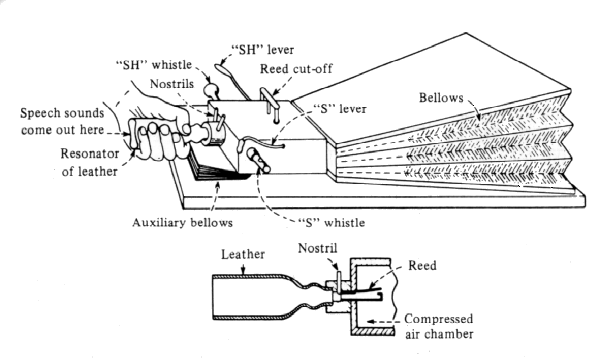
\includegraphics[width = .25\textwidth]{figures/Einleitung/kratzenstein.png}
	\caption{Kratzensteins Resonator \cite[S. 5]{lemmetty1999review} }
	\label{fig:kratzenstein}
\end{figure}

Weitere Meilensteine waren die Entwicklung elektronischer Filter sowie der Einsatz moderner Computertechnik. 

Heutzutage kommen Systeme zur Sprachsynthese zum Beispiel in Navigationsger\"aten und Smartphones zum Einsatz.

%-------------------------------------------------
\section*{Quelle-Filter-Modell}
%-------------------------------------------------

Das Quelle-Filter-Modell versucht eine Zerlegung von Sprachsignalen in Anregungssignale und Filterstrukturen. Durch geeignete Wahl der Modellparameter soll eine m\"oglichst gute Modellierung des menschlichen Artikulationstrakts erreicht werden. 

Die Struktur des Modells, wie es hier verwendet wird, ist in Abbildung \ref{fig:QFM} gezeigt.

\begin{figure}[H]
	\centering
	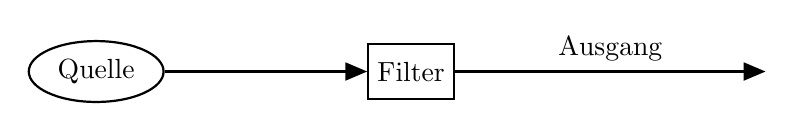
\begin{tikzpicture}[auto, thick, node distance=2cm, >=triangle 45]
\draw
% Block setzen
node at (-1,0)[elipse](input) {Quelle} 
node at (3,0)[block] (filter) {Filter};
% Block verbinden
\draw[->](input) -- node {}(filter);
\draw[->](filter) -- node {Ausgang}(7.5,0);

\end{tikzpicture}
	\caption{Verwendetes Quelle-Filter-Modell}
	\label{fig:QFM}
\end{figure}



%-------------------------------------------------
\section*{Analyse}

Zur Parametrisierung des in Abbildung \ref{fig:QFM} dargestellten Modells m\"ussen reale Sprachsignale analysiert werden.

Der Schwerpunkt liegt hierbei auf der Bestimmung der Filterparameter. Es werden prim\"ar Bandpassfilter 2. Ordnung eingesetzt. Die drei charakteristischen Parameter sind Mittenfrequenz, Bandbreite und Grundverst\"arkung.

Die Mittenfrequenz wird als Formantfrequenz bezeichnet. Um diese zu bestimmen, wurden verschiedene Analysemethoden verwendet. Von der Software Praat wurde der fertig implementierte Burg-Algorithmus bereitgestellt, selbst nachprogrammiert wurde der Cepstrum-Algorithmus. Das dabei gewonnene gegl\"attete Spektrum ist in Abbildung \ref{fig:spektrum} dargestellt.
{
	%\setlength{cmd}{len}
\begin{figure}[H]
	\centering
	\begin{axis}[%
width=0.8\columnwidth,
%height=0.197\textwidth,
at={(0\textwidth,0\textwidth)},
scale only axis,
xmin=0,
xmax=3500,
xlabel={Frequenz in Hz},
ymin=-0.7,
ymax=-0.1,
ylabel={Amplitudenspektrum},
%title={$\text{Formanten f\"ur den Vokal \enquote}{\text{i}}$}
]
\addplot [color=blue,solid,forget plot]
  table[row sep=crcr]{%
0	-0.1870873676787\\
172.265625	-0.124606592043381\\
344.53125	-0.278971980502043\\
516.796875	-0.408552272077687\\
689.0625	-0.487382878228641\\
861.328125	-0.523481417803874\\
1033.59375	-0.543768039416707\\
1205.859375	-0.581938318802905\\
1378.125	-0.595244109407637\\
1550.390625	-0.586787106479387\\
1722.65625	-0.594810571612354\\
1894.921875	-0.52854416045969\\
2067.1875	-0.433815573300611\\
2239.453125	-0.254441702688233\\
2411.71875	-0.561540523033787\\
2583.984375	-0.481655266112142\\
2756.25	-0.448850362610164\\
2928.515625	-0.336331361460825\\
3100.78125	-0.265846718893173\\
3273.046875	-0.36601407031051\\
3445.3125	-0.27154698246101\\
3617.578125	-0.265874222160239\\
3789.84375	-0.505589755361803\\
3962.109375	-0.493064840245526\\
4134.375	-0.488697668563952\\
4306.640625	-0.50241665499048\\
4478.90625	-0.443373885568908\\
4651.171875	-0.376730549785729\\
4823.4375	-0.285470253800668\\
4995.703125	-0.251392727331721\\
5167.96875	-0.247911926741615\\
5340.234375	-0.224874455672336\\
5512.5	-0.157800464770028\\
5684.765625	-0.1800294293081\\
5857.03125	-0.247664864724133\\
6029.296875	-0.263915165617128\\
6201.5625	-0.176428925969494\\
6373.828125	-0.141180205091637\\
6546.09375	-0.387777081282331\\
6718.359375	-0.370707943332816\\
6890.625	-0.320616446386987\\
7062.890625	-0.243273513831002\\
7235.15625	-0.445014028915396\\
7407.421875	-0.503895570867559\\
7579.6875	-0.61510170950748\\
7751.953125	-0.560142047194254\\
7924.21875	-0.50446638188819\\
8096.484375	-0.621396958672453\\
8268.75	-0.689487013486006\\
8441.015625	-0.736726881637801\\
8613.28125	-0.625933838446098\\
8785.546875	-0.423570746609167\\
8957.8125	-0.457258481538982\\
9130.078125	-0.598761118950131\\
9302.34375	-0.50140752514791\\
9474.609375	-0.535967282788022\\
9646.875	-0.642958627677039\\
9819.140625	-0.4571264964318\\
9991.40625	-0.557372901488328\\
10163.671875	-0.690265690621624\\
10335.9375	-0.607809935105308\\
10508.203125	-0.739912404869531\\
10680.46875	-0.761826770053667\\
10852.734375	-0.597000622324391\\
11025	-0.469328678220118\\
11197.265625	-0.520478989918416\\
11369.53125	-0.518590660824286\\
11541.796875	-0.580155608736083\\
11714.0625	-0.646321232890602\\
11886.328125	-0.8012588907925\\
12058.59375	-0.700165049834895\\
12230.859375	-0.732953667034508\\
12403.125	-0.616466415278129\\
12575.390625	-0.560488197291204\\
12747.65625	-0.778365897312256\\
12919.921875	-0.755240265914003\\
13092.1875	-0.801364747751031\\
13264.453125	-0.857226371707966\\
13436.71875	-0.919279234333996\\
13608.984375	-0.946009484822061\\
13781.25	-0.893603138858667\\
13953.515625	-0.898704826963627\\
14125.78125	-0.913917797749607\\
14298.046875	-0.907415428936837\\
14470.3125	-0.850633074901554\\
14642.578125	-0.822242106711636\\
14814.84375	-0.912518836774858\\
14987.109375	-0.923232400919938\\
15159.375	-0.924110832271203\\
15331.640625	-0.923816100660652\\
15503.90625	-0.875929484987136\\
15676.171875	-0.862948400601403\\
15848.4375	-0.889977020534071\\
16020.703125	-0.921276581984284\\
16192.96875	-0.937071633237406\\
16365.234375	-0.930745205138123\\
16537.5	-0.951577204448038\\
16709.765625	-0.9371298296321\\
16882.03125	-0.918140206991247\\
17054.296875	-0.945910236340733\\
17226.5625	-0.923388271307007\\
17398.828125	-0.917916735778229\\
17571.09375	-0.959438227031189\\
17743.359375	-0.93134469589279\\
17915.625	-0.967436401730026\\
18087.890625	-0.940612412084777\\
18260.15625	-0.939514655053184\\
18432.421875	-0.934068294397959\\
18604.6875	-0.963882556330112\\
18776.953125	-0.958688859710452\\
18949.21875	-0.958339331785018\\
19121.484375	-0.955436833401938\\
19293.75	-0.96022875373091\\
19466.015625	-0.96897250385543\\
19638.28125	-0.979304288015029\\
19810.546875	-0.973442142568704\\
19982.8125	-0.966452999180048\\
20155.078125	-0.970027664140936\\
20327.34375	-0.992586844959336\\
20499.609375	-0.975733951179023\\
20671.875	-0.992750105749142\\
20844.140625	-1\\
21016.40625	-0.993068132208889\\
21188.671875	-0.989064179905442\\
21360.9375	-0.982378327232826\\
21533.203125	-0.991285556593491\\
21705.46875	-0.992114960027848\\
21877.734375	-0.982487871624791\\
};
\end{axis}
	\caption{Gegl\"attetes Spektrum des Vokals i}
	\label{fig:spektrum}
\end{figure}
}

%-------------------------------------------------
\section*{Synthese}

Zur Synthese von Einzellauten werden verschiedene Quelle-Filter-Modelle verwendet.

\subsection*{Synthetisierbare Einzellaute}
Implementiert wurden folgende Laute: Vokale, Diphtonge (/au/, /ei/, /eu/), stimmlose Frikative (/ch/, /f/, /s/, /sch/), stimmhafte Frikative (/w/), stimmhafte Plosive (/b/, /d/, /g/), stimmlose Plosive (/k/, /t/, /p/), Liquide (/l/, /r/) sowie Nasale (/m/, /n/).

Allerdings k\"onnen stimmhafte Plosive nur in Verbindung mit einem darauffolgenden Vokal synthetisiert werden.

\subsection*{Vokale}
Zur Synthese von Vokallauten wird ein periodisches breitbandiges Anregungssignal als Quelle verwendet. Die Signalformung wird mittels Bandpassfilter in Reihenschaltung realisiert.


Das Anregungssignal f\"ur die stimmhaften Laute soll den glottalen Luftstrom nachbilden. Dazu wurde eine von Paul Taylor vorgeschlagene Formel benutzt.


\begin{figure}[H]
	\centering
	% This file was created by matlab2tikz.
% Minimal pgfplots version: 1.3
%
%The latest updates can be retrieved from
%  http://www.mathworks.com/matlabcentral/fileexchange/22022-matlab2tikz
%where you can also make suggestions and rate matlab2tikz.
%
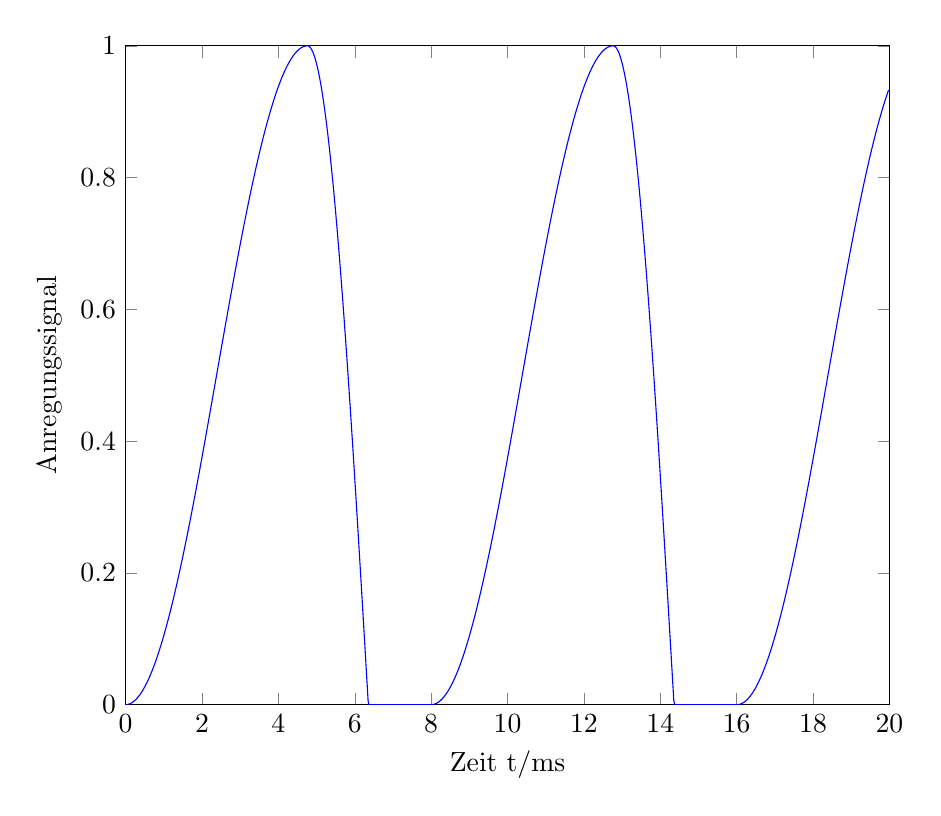
\begin{tikzpicture}

\begin{axis}[%
width=0.8\columnwidth,
%height=0.5\columnwidth,
at={(0\textwidth,0\textwidth)},
scale only axis,
xmin=0,
xmax=20,
xlabel={Zeit t/ms},
ymin=0,
ymax=1,
ylabel={Anregungssignal}
]
\addplot [color=blue,solid,forget plot]
  table[row sep=crcr]{%
0	0\\
0.0226757369614512	5.59490948632835e-005\\
0.0453514739229025	0.000223783858248339\\
0.0680272108843537	0.00050346672934265\\
0.090702947845805	0.000894935116132423\\
0.113378684807256	0.00139810140940994\\
0.136054421768707	0.00201285300238047\\
0.158730158730159	0.00273905231586336\\
0.18140589569161	0.00357653682908132\\
0.204081632653061	0.00452511911603259\\
0.226757369614512	0.00558458688743574\\
0.249433106575964	0.00675470303823927\\
0.272108843537415	0.00803520570068517\\
0.294784580498866	0.00942580830291367\\
0.317460317460317	0.0109261996330972\\
0.340136054421769	0.0125360439090882\\
0.36281179138322	0.0142549808535663\\
0.385487528344671	0.0160826257746667\\
0.408163265306122	0.0180185696520734\\
0.430839002267574	0.0200623792285555\\
0.453514739229025	0.0222135971069296\\
0.476190476190476	0.0244717418524232\\
0.498866213151927	0.0268363081004179\\
0.521541950113379	0.0293067666695484\\
0.54421768707483	0.0318825646801314\\
0.566893424036281	0.0345631256778979\\
0.589569160997732	0.0373478497630017\\
0.612244897959184	0.0402361137242747\\
0.634920634920635	0.0432272711786995\\
0.657596371882086	0.0463206527160676\\
0.680272108843537	0.0495155660487904\\
0.702947845804989	0.0528112961668316\\
0.72562358276644	0.056207105497723\\
0.748299319727891	0.059702234071631\\
0.770975056689342	0.0632958996914351\\
0.793650793650794	0.0669872981077806\\
0.816326530612245	0.070775603199067\\
0.839002267573696	0.0746599671563302\\
0.861678004535147	0.0786395206729804\\
0.884353741496599	0.0827133731393486\\
0.90702947845805	0.0868806128420025\\
0.929705215419501	0.0911403071677843\\
0.952380952380952	0.0954915028125263\\
0.975056689342404	0.0999332259943968\\
0.997732426303855	0.104464482671829\\
1.02040816326531	0.109084258765985\\
1.04308390022676	0.1137915203877\\
1.06575963718821	0.118585214068867\\
1.08843537414966	0.123464266998194\\
1.11111111111111	0.128427587261303\\
1.13378684807256	0.133474064085087\\
1.15646258503401	0.138602568086304\\
1.17913832199546	0.143811951524328\\
1.20181405895692	0.149101048558004\\
1.22448979591837	0.154468675506568\\
1.24716553287982	0.15991363111454\\
1.26984126984127	0.165434696820571\\
1.29251700680272	0.171030637030144\\
1.31519274376417	0.1767001993921\\
1.33786848072562	0.182442115078911\\
1.36054421768707	0.188255099070633\\
1.38321995464853	0.194137850442497\\
1.40589569160998	0.200089052656043\\
1.42857142857143	0.206107373853763\\
1.45124716553288	0.212191467157163\\
1.47392290249433	0.218339970968189\\
1.49659863945578	0.224551509273949\\
1.51927437641723	0.230824691954659\\
1.54195011337868	0.237158115094748\\
1.56462585034014	0.243550361297047\\
1.58730158730159	0.25\\
1.60997732426304	0.256505587797816\\
1.63265306122449	0.263065668763501\\
1.65532879818594	0.269678774774684\\
1.67800453514739	0.276343425842184\\
1.70068027210884	0.283058130441221\\
1.72335600907029	0.289821385845217\\
1.74603174603175	0.2966316784621\\
1.7687074829932	0.303487484173038\\
1.79138321995465	0.310387268673536\\
1.8140589569161	0.317329487816802\\
1.83673469387755	0.324312587959329\\
1.859410430839	0.331335006308585\\
1.88208616780045	0.33839517127277\\
1.9047619047619	0.345491502812526\\
1.92743764172336	0.352622412794548\\
1.95011337868481	0.359786305346999\\
1.97278911564626	0.366981577216662\\
1.99546485260771	0.374206618127746\\
2.01814058956916	0.381459811142251\\
2.04081632653061	0.388739533021843\\
2.06349206349206	0.39604415459112\\
2.08616780045351	0.403372041102223\\
2.10884353741497	0.410721552600682\\
2.13151927437642	0.418091044292431\\
2.15419501133787	0.425478866911913\\
2.17687074829932	0.432883367091172\\
2.19954648526077	0.440302887729878\\
2.22222222222222	0.447735768366173\\
2.24489795918367	0.455180345548283\\
2.26757369614512	0.462634953206788\\
2.29024943310658	0.470097923027483\\
2.31292517006803	0.477567584824742\\
2.33560090702948	0.485042266915301\\
2.35827664399093	0.492520296492368\\
2.38095238095238	0.5\\
2.40362811791383	0.507479703507632\\
2.42630385487528	0.514957733084699\\
2.44897959183673	0.522432415175257\\
2.47165532879819	0.529902076972517\\
2.49433106575964	0.537365046793212\\
2.51700680272109	0.544819654451717\\
2.53968253968254	0.552264231633827\\
2.56235827664399	0.559697112270122\\
2.58503401360544	0.567116632908828\\
2.60770975056689	0.574521133088087\\
2.63038548752834	0.581908955707569\\
2.6530612244898	0.589278447399318\\
2.67573696145125	0.596627958897777\\
2.6984126984127	0.60395584540888\\
2.72108843537415	0.611260466978157\\
2.7437641723356	0.618540188857749\\
2.76643990929705	0.625793381872254\\
2.7891156462585	0.633018422783338\\
2.81179138321995	0.640213694653001\\
2.83446712018141	0.647377587205452\\
2.85714285714286	0.654508497187474\\
2.87981859410431	0.66160482872723\\
2.90249433106576	0.668664993691415\\
2.92517006802721	0.675687412040671\\
2.94784580498866	0.682670512183197\\
2.97052154195011	0.689612731326464\\
2.99319727891156	0.696512515826962\\
3.01587301587302	0.7033683215379\\
3.03854875283447	0.710178614154783\\
3.06122448979592	0.716941869558779\\
3.08390022675737	0.723656574157816\\
3.10657596371882	0.730321225225316\\
3.12925170068027	0.736934331236499\\
3.15192743764172	0.743494412202184\\
3.17460317460317	0.75\\
3.19727891156463	0.756449638702953\\
3.21995464852608	0.762841884905252\\
3.24263038548753	0.769175308045341\\
3.26530612244898	0.775448490726051\\
3.28798185941043	0.781660029031811\\
3.31065759637188	0.787808532842837\\
3.33333333333333	0.793892626146236\\
3.35600907029478	0.799910947343957\\
3.37868480725624	0.805862149557503\\
3.40136054421769	0.811744900929367\\
3.42403628117914	0.817557884921089\\
3.44671201814059	0.8232998006079\\
3.46938775510204	0.828969362969856\\
3.49206349206349	0.834565303179429\\
3.51473922902494	0.84008636888546\\
3.53741496598639	0.845531324493432\\
3.56009070294785	0.850898951441996\\
3.5827664399093	0.856188048475672\\
3.60544217687075	0.861397431913696\\
3.6281179138322	0.866525935914913\\
3.65079365079365	0.871572412738697\\
3.6734693877551	0.876535733001805\\
3.69614512471655	0.881414785931133\\
3.718820861678	0.8862084796123\\
3.74149659863946	0.890915741234015\\
3.76417233560091	0.89553551732817\\
3.78684807256236	0.900066774005603\\
3.80952380952381	0.904508497187474\\
3.83219954648526	0.908859692832216\\
3.85487528344671	0.913119387157997\\
3.87755102040816	0.917286626860651\\
3.90022675736961	0.921360479327019\\
3.92290249433107	0.92534003284367\\
3.94557823129252	0.929224396800933\\
3.96825396825397	0.933012701892219\\
3.99092970521542	0.936704100308565\\
4.01360544217687	0.940297765928369\\
4.03628117913832	0.943792894502277\\
4.05895691609977	0.947188703833168\\
4.08163265306122	0.95048443395121\\
4.10430839002268	0.953679347283932\\
4.12698412698413	0.9567727288213\\
4.14965986394558	0.959763886275725\\
4.17233560090703	0.962652150236998\\
4.19501133786848	0.965436874322102\\
4.21768707482993	0.968117435319868\\
4.24036281179138	0.970693233330452\\
4.26303854875283	0.973163691899582\\
4.28571428571429	0.975528258147577\\
4.30839002267574	0.97778640289307\\
4.33106575963719	0.979937620771445\\
4.35374149659864	0.981981430347927\\
4.37641723356009	0.983917374225333\\
4.39909297052154	0.985745019146434\\
4.42176870748299	0.987463956090912\\
4.44444444444444	0.989073800366903\\
4.4671201814059	0.990574191697086\\
4.48979591836735	0.991964794299315\\
4.5124716553288	0.993245296961761\\
4.53514739229025	0.994415413112564\\
4.5578231292517	0.995474880883967\\
4.58049886621315	0.996423463170919\\
4.6031746031746	0.997260947684137\\
4.62585034013605	0.99798714699762\\
4.64852607709751	0.99860189859059\\
4.67120181405896	0.999105064883868\\
4.69387755102041	0.999496533270657\\
4.71655328798186	0.999776216141752\\
4.73922902494331	0.999944050905137\\
4.76190476190476	1\\
4.78458049886621	0.999750023601623\\
4.80725623582766	0.999000219382892\\
4.82993197278912	0.997750962210523\\
4.85260770975057	0.996002876654134\\
4.87528344671202	0.993756836673986\\
4.89795918367347	0.99101396518405\\
4.92063492063492	0.987775633490598\\
4.94331065759637	0.984043460606618\\
4.96598639455782	0.97981931244238\\
4.98866213151927	0.975105300872574\\
5.01133786848073	0.969903782680467\\
5.03401360544218	0.964217358379627\\
5.05668934240363	0.958048870913786\\
5.07936507936508	0.951401404235506\\
5.10204081632653	0.944278281764342\\
5.12471655328798	0.936683064725297\\
5.14739229024943	0.928619550368371\\
5.17006802721088	0.920091770070118\\
5.19274376417234	0.911103987318148\\
5.21541950113379	0.901660695579585\\
5.23809523809524	0.891766616054545\\
5.26077097505669	0.881426695315756\\
5.28344671201814	0.870646102835511\\
5.30612244897959	0.85943022840117\\
5.32879818594104	0.847784679420526\\
5.35147392290249	0.83571527811836\\
5.37414965986395	0.82322805862561\\
5.3968253968254	0.810329263962584\\
5.41950113378685	0.797025342917748\\
5.4421768707483	0.783322946823637\\
5.46485260770975	0.7692289262315\\
5.4875283446712	0.75475032748635\\
5.51020408163265	0.739894389204122\\
5.5328798185941	0.72466853865271\\
5.55555555555556	0.709080388038678\\
5.57823129251701	0.693137730701524\\
5.60090702947846	0.67684853721737\\
5.62358276643991	0.660220951414055\\
5.64625850340136	0.643263286299606\\
5.66893424036281	0.625984019906122\\
5.69160997732426	0.608391791051163\\
5.71428571428571	0.590495395018746\\
5.73696145124717	0.572303779162119\\
5.75963718820862	0.553826038430508\\
5.78231292517007	0.535071410822067\\
5.80498866213152	0.516049272765325\\
5.82766439909297	0.4967691344314\\
5.85034013605442	0.477240634979375\\
5.87301587301587	0.457473537737168\\
5.89569160997732	0.437477725320327\\
5.91836734693878	0.417263194691197\\
5.94104308390023	0.396840052160897\\
5.96371882086168	0.376218508336656\\
5.98639455782313	0.355408873016981\\
6.00907029478458	0.334421550037251\\
6.03174603174603	0.313267032068285\\
6.05442176870748	0.291955895370506\\
6.07709750566893	0.270498794506307\\
6.09977324263039	0.248906457013277\\
6.12244897959184	0.227189678040932\\
6.14512471655329	0.205359314953658\\
6.16780045351474	0.183426281902533\\
6.19047619047619	0.161401544368772\\
6.21315192743764	0.139296113681505\\
6.23582766439909	0.117121041512625\\
6.25850340136054	0.0948874143514825\\
6.281179138322	0.0726063479621576\\
6.30385487528345	0.050288981826108\\
6.3265306122449	0.0279464735729472\\
6.34920634920635	0.00558999340216533\\
6.3718820861678	0\\
6.39455782312925	0\\
6.4172335600907	0\\
6.43990929705215	0\\
6.46258503401361	0\\
6.48526077097506	0\\
6.50793650793651	0\\
6.53061224489796	0\\
6.55328798185941	0\\
6.57596371882086	0\\
6.59863945578231	0\\
6.62131519274376	0\\
6.64399092970522	0\\
6.66666666666667	0\\
6.68934240362812	0\\
6.71201814058957	0\\
6.73469387755102	0\\
6.75736961451247	0\\
6.78004535147392	0\\
6.80272108843537	0\\
6.82539682539683	0\\
6.84807256235828	0\\
6.87074829931973	0\\
6.89342403628118	0\\
6.91609977324263	0\\
6.93877551020408	0\\
6.96145124716553	0\\
6.98412698412698	0\\
7.00680272108844	0\\
7.02947845804989	0\\
7.05215419501134	0\\
7.07482993197279	0\\
7.09750566893424	0\\
7.12018140589569	0\\
7.14285714285714	0\\
7.16553287981859	0\\
7.18820861678005	0\\
7.2108843537415	0\\
7.23356009070295	0\\
7.2562358276644	0\\
7.27891156462585	0\\
7.3015873015873	0\\
7.32426303854875	0\\
7.3469387755102	0\\
7.36961451247166	0\\
7.39229024943311	0\\
7.41496598639456	0\\
7.43764172335601	0\\
7.46031746031746	0\\
7.48299319727891	0\\
7.50566893424036	0\\
7.52834467120181	0\\
7.55102040816327	0\\
7.57369614512472	0\\
7.59637188208617	0\\
7.61904761904762	0\\
7.64172335600907	0\\
7.66439909297052	0\\
7.68707482993197	0\\
7.70975056689342	0\\
7.73242630385487	0\\
7.75510204081633	0\\
7.77777777777778	0\\
7.80045351473923	0\\
7.82312925170068	0\\
7.84580498866213	0\\
7.86848072562358	0\\
7.89115646258503	0\\
7.91383219954649	0\\
7.93650793650794	0\\
7.95918367346939	0\\
7.98185941043084	0\\
8.00453514739229	0\\
8.02721088435374	5.59490948632835e-005\\
8.04988662131519	0.000223783858248339\\
8.07256235827664	0.00050346672934265\\
8.09523809523809	0.000894935116132423\\
8.11791383219955	0.00139810140940994\\
8.140589569161	0.00201285300238047\\
8.16326530612245	0.00273905231586336\\
8.1859410430839	0.00357653682908132\\
8.20861678004535	0.00452511911603259\\
8.2312925170068	0.00558458688743574\\
8.25396825396825	0.00675470303823927\\
8.2766439909297	0.00803520570068517\\
8.29931972789116	0.00942580830291367\\
8.32199546485261	0.0109261996330972\\
8.34467120181406	0.0125360439090882\\
8.36734693877551	0.0142549808535663\\
8.39002267573696	0.0160826257746667\\
8.41269841269841	0.0180185696520734\\
8.43537414965986	0.0200623792285555\\
8.45804988662132	0.0222135971069296\\
8.48072562358277	0.0244717418524232\\
8.50340136054422	0.0268363081004179\\
8.52607709750567	0.0293067666695484\\
8.54875283446712	0.0318825646801314\\
8.57142857142857	0.0345631256778979\\
8.59410430839002	0.0373478497630017\\
8.61678004535147	0.0402361137242747\\
8.63945578231293	0.0432272711786995\\
8.66213151927438	0.0463206527160676\\
8.68480725623583	0.0495155660487904\\
8.70748299319728	0.0528112961668316\\
8.73015873015873	0.056207105497723\\
8.75283446712018	0.059702234071631\\
8.77551020408163	0.0632958996914351\\
8.79818594104308	0.0669872981077806\\
8.82086167800454	0.070775603199067\\
8.84353741496599	0.0746599671563302\\
8.86621315192744	0.0786395206729804\\
8.88888888888889	0.0827133731393486\\
8.91156462585034	0.0868806128420025\\
8.93424036281179	0.0911403071677843\\
8.95691609977324	0.0954915028125263\\
8.97959183673469	0.0999332259943968\\
9.00226757369614	0.104464482671829\\
9.0249433106576	0.109084258765985\\
9.04761904761905	0.1137915203877\\
9.0702947845805	0.118585214068867\\
9.09297052154195	0.123464266998194\\
9.1156462585034	0.128427587261303\\
9.13832199546485	0.133474064085087\\
9.1609977324263	0.138602568086304\\
9.18367346938775	0.143811951524328\\
9.20634920634921	0.149101048558004\\
9.22902494331066	0.154468675506568\\
9.25170068027211	0.15991363111454\\
9.27437641723356	0.165434696820571\\
9.29705215419501	0.171030637030144\\
9.31972789115646	0.1767001993921\\
9.34240362811791	0.182442115078911\\
9.36507936507937	0.188255099070633\\
9.38775510204082	0.194137850442497\\
9.41043083900227	0.200089052656043\\
9.43310657596372	0.206107373853763\\
9.45578231292517	0.212191467157163\\
9.47845804988662	0.218339970968189\\
9.50113378684807	0.224551509273949\\
9.52380952380952	0.230824691954659\\
9.54648526077098	0.237158115094748\\
9.56916099773243	0.243550361297047\\
9.59183673469388	0.25\\
9.61451247165533	0.256505587797816\\
9.63718820861678	0.263065668763501\\
9.65986394557823	0.269678774774684\\
9.68253968253968	0.276343425842184\\
9.70521541950113	0.283058130441221\\
9.72789115646258	0.289821385845217\\
9.75056689342404	0.2966316784621\\
9.77324263038549	0.303487484173038\\
9.79591836734694	0.310387268673536\\
9.81859410430839	0.317329487816802\\
9.84126984126984	0.324312587959329\\
9.86394557823129	0.331335006308585\\
9.88662131519274	0.33839517127277\\
9.90929705215419	0.345491502812526\\
9.93197278911565	0.352622412794548\\
9.9546485260771	0.359786305346999\\
9.97732426303855	0.366981577216662\\
10	0.374206618127746\\
10.0226757369615	0.381459811142251\\
10.0453514739229	0.388739533021843\\
10.0680272108844	0.39604415459112\\
10.0907029478458	0.403372041102223\\
10.1133786848073	0.410721552600682\\
10.1360544217687	0.418091044292431\\
10.1587301587302	0.425478866911913\\
10.1814058956916	0.432883367091172\\
10.2040816326531	0.440302887729878\\
10.2267573696145	0.447735768366173\\
10.249433106576	0.455180345548283\\
10.2721088435374	0.462634953206788\\
10.2947845804989	0.470097923027483\\
10.3174603174603	0.477567584824742\\
10.3401360544218	0.485042266915301\\
10.3628117913832	0.492520296492368\\
10.3854875283447	0.5\\
10.4081632653061	0.507479703507632\\
10.4308390022676	0.514957733084699\\
10.453514739229	0.522432415175257\\
10.4761904761905	0.529902076972517\\
10.4988662131519	0.537365046793212\\
10.5215419501134	0.544819654451717\\
10.5442176870748	0.552264231633827\\
10.5668934240363	0.559697112270122\\
10.5895691609977	0.567116632908828\\
10.6122448979592	0.574521133088087\\
10.6349206349206	0.581908955707569\\
10.6575963718821	0.589278447399318\\
10.6802721088435	0.596627958897777\\
10.702947845805	0.60395584540888\\
10.7256235827664	0.611260466978157\\
10.7482993197279	0.618540188857749\\
10.7709750566893	0.625793381872254\\
10.7936507936508	0.633018422783338\\
10.8163265306122	0.640213694653001\\
10.8390022675737	0.647377587205452\\
10.8616780045351	0.654508497187474\\
10.8843537414966	0.66160482872723\\
10.9070294784581	0.668664993691415\\
10.9297052154195	0.675687412040671\\
10.952380952381	0.682670512183197\\
10.9750566893424	0.689612731326464\\
10.9977324263039	0.696512515826962\\
11.0204081632653	0.7033683215379\\
11.0430839002268	0.710178614154783\\
11.0657596371882	0.716941869558779\\
11.0884353741497	0.723656574157816\\
11.1111111111111	0.730321225225316\\
11.1337868480726	0.736934331236499\\
11.156462585034	0.743494412202184\\
11.1791383219955	0.75\\
11.2018140589569	0.756449638702953\\
11.2244897959184	0.762841884905252\\
11.2471655328798	0.769175308045341\\
11.2698412698413	0.775448490726051\\
11.2925170068027	0.781660029031811\\
11.3151927437642	0.787808532842837\\
11.3378684807256	0.793892626146236\\
11.3605442176871	0.799910947343957\\
11.3832199546485	0.805862149557503\\
11.40589569161	0.811744900929367\\
11.4285714285714	0.817557884921089\\
11.4512471655329	0.8232998006079\\
11.4739229024943	0.828969362969856\\
11.4965986394558	0.834565303179429\\
11.5192743764172	0.84008636888546\\
11.5419501133787	0.845531324493432\\
11.5646258503401	0.850898951441996\\
11.5873015873016	0.856188048475672\\
11.609977324263	0.861397431913696\\
11.6326530612245	0.866525935914913\\
11.6553287981859	0.871572412738697\\
11.6780045351474	0.876535733001805\\
11.7006802721088	0.881414785931133\\
11.7233560090703	0.8862084796123\\
11.7460317460317	0.890915741234015\\
11.7687074829932	0.89553551732817\\
11.7913832199546	0.900066774005603\\
11.8140589569161	0.904508497187474\\
11.8367346938776	0.908859692832216\\
11.859410430839	0.913119387157997\\
11.8820861678005	0.917286626860651\\
11.9047619047619	0.921360479327019\\
11.9274376417234	0.92534003284367\\
11.9501133786848	0.929224396800933\\
11.9727891156463	0.933012701892219\\
11.9954648526077	0.936704100308565\\
12.0181405895692	0.940297765928369\\
12.0408163265306	0.943792894502277\\
12.0634920634921	0.947188703833168\\
12.0861678004535	0.95048443395121\\
12.108843537415	0.953679347283932\\
12.1315192743764	0.9567727288213\\
12.1541950113379	0.959763886275725\\
12.1768707482993	0.962652150236998\\
12.1995464852608	0.965436874322102\\
12.2222222222222	0.968117435319868\\
12.2448979591837	0.970693233330452\\
12.2675736961451	0.973163691899582\\
12.2902494331066	0.975528258147577\\
12.312925170068	0.97778640289307\\
12.3356009070295	0.979937620771445\\
12.3582766439909	0.981981430347927\\
12.3809523809524	0.983917374225333\\
12.4036281179138	0.985745019146434\\
12.4263038548753	0.987463956090912\\
12.4489795918367	0.989073800366903\\
12.4716553287982	0.990574191697086\\
12.4943310657596	0.991964794299315\\
12.5170068027211	0.993245296961761\\
12.5396825396825	0.994415413112564\\
12.562358276644	0.995474880883967\\
12.5850340136054	0.996423463170919\\
12.6077097505669	0.997260947684137\\
12.6303854875283	0.99798714699762\\
12.6530612244898	0.99860189859059\\
12.6757369614512	0.999105064883868\\
12.6984126984127	0.999496533270657\\
12.7210884353741	0.999776216141752\\
12.7437641723356	0.999944050905137\\
12.7664399092971	1\\
12.7891156462585	0.999750023601623\\
12.81179138322	0.999000219382892\\
12.8344671201814	0.997750962210523\\
12.8571428571429	0.996002876654134\\
12.8798185941043	0.993756836673986\\
12.9024943310658	0.99101396518405\\
12.9251700680272	0.987775633490598\\
12.9478458049887	0.984043460606618\\
12.9705215419501	0.97981931244238\\
12.9931972789116	0.975105300872574\\
13.015873015873	0.969903782680467\\
13.0385487528345	0.964217358379627\\
13.0612244897959	0.958048870913786\\
13.0839002267574	0.951401404235506\\
13.1065759637188	0.944278281764342\\
13.1292517006803	0.936683064725297\\
13.1519274376417	0.928619550368371\\
13.1746031746032	0.920091770070118\\
13.1972789115646	0.911103987318148\\
13.2199546485261	0.901660695579585\\
13.2426303854875	0.891766616054545\\
13.265306122449	0.881426695315756\\
13.2879818594104	0.870646102835511\\
13.3106575963719	0.85943022840117\\
13.3333333333333	0.847784679420526\\
13.3560090702948	0.83571527811836\\
13.3786848072562	0.82322805862561\\
13.4013605442177	0.810329263962584\\
13.4240362811791	0.797025342917748\\
13.4467120181406	0.783322946823637\\
13.469387755102	0.7692289262315\\
13.4920634920635	0.75475032748635\\
13.5147392290249	0.739894389204122\\
13.5374149659864	0.72466853865271\\
13.5600907029478	0.709080388038678\\
13.5827664399093	0.693137730701524\\
13.6054421768707	0.67684853721737\\
13.6281179138322	0.660220951414055\\
13.6507936507937	0.643263286299606\\
13.6734693877551	0.625984019906122\\
13.6961451247166	0.608391791051163\\
13.718820861678	0.590495395018746\\
13.7414965986395	0.572303779162119\\
13.7641723356009	0.553826038430508\\
13.7868480725624	0.535071410822067\\
13.8095238095238	0.516049272765325\\
13.8321995464853	0.4967691344314\\
13.8548752834467	0.477240634979375\\
13.8775510204082	0.457473537737168\\
13.9002267573696	0.437477725320327\\
13.9229024943311	0.417263194691197\\
13.9455782312925	0.396840052160897\\
13.968253968254	0.376218508336656\\
13.9909297052154	0.355408873016981\\
14.0136054421769	0.334421550037251\\
14.0362811791383	0.313267032068285\\
14.0589569160998	0.291955895370506\\
14.0816326530612	0.270498794506307\\
14.1043083900227	0.248906457013277\\
14.1269841269841	0.227189678040932\\
14.1496598639456	0.205359314953658\\
14.172335600907	0.183426281902533\\
14.1950113378685	0.161401544368772\\
14.2176870748299	0.139296113681505\\
14.2403628117914	0.117121041512625\\
14.2630385487528	0.0948874143514825\\
14.2857142857143	0.0726063479621576\\
14.3083900226757	0.050288981826108\\
14.3310657596372	0.0279464735729472\\
14.3537414965986	0.00558999340216533\\
14.3764172335601	0\\
14.3990929705215	0\\
14.421768707483	0\\
14.4444444444444	0\\
14.4671201814059	0\\
14.4897959183673	0\\
14.5124716553288	0\\
14.5351473922902	0\\
14.5578231292517	0\\
14.5804988662132	0\\
14.6031746031746	0\\
14.6258503401361	0\\
14.6485260770975	0\\
14.671201814059	0\\
14.6938775510204	0\\
14.7165532879819	0\\
14.7392290249433	0\\
14.7619047619048	0\\
14.7845804988662	0\\
14.8072562358277	0\\
14.8299319727891	0\\
14.8526077097506	0\\
14.875283446712	0\\
14.8979591836735	0\\
14.9206349206349	0\\
14.9433106575964	0\\
14.9659863945578	0\\
14.9886621315193	0\\
15.0113378684807	0\\
15.0340136054422	0\\
15.0566893424036	0\\
15.0793650793651	0\\
15.1020408163265	0\\
15.124716553288	0\\
15.1473922902494	0\\
15.1700680272109	0\\
15.1927437641723	0\\
15.2154195011338	0\\
15.2380952380952	0\\
15.2607709750567	0\\
15.2834467120181	0\\
15.3061224489796	0\\
15.328798185941	0\\
15.3514739229025	0\\
15.3741496598639	0\\
15.3968253968254	0\\
15.4195011337868	0\\
15.4421768707483	0\\
15.4648526077098	0\\
15.4875283446712	0\\
15.5102040816327	0\\
15.5328798185941	0\\
15.5555555555556	0\\
15.578231292517	0\\
15.6009070294785	0\\
15.6235827664399	0\\
15.6462585034014	0\\
15.6689342403628	0\\
15.6916099773243	0\\
15.7142857142857	0\\
15.7369614512472	0\\
15.7596371882086	0\\
15.7823129251701	0\\
15.8049886621315	0\\
15.827664399093	0\\
15.8503401360544	0\\
15.8730158730159	0\\
15.8956916099773	0\\
15.9183673469388	0\\
15.9410430839002	0\\
15.9637188208617	0\\
15.9863945578231	0\\
16.0090702947846	0\\
16.031746031746	5.59490948632835e-005\\
16.0544217687075	0.000223783858248339\\
16.0770975056689	0.00050346672934265\\
16.0997732426304	0.000894935116132423\\
16.1224489795918	0.00139810140940994\\
16.1451247165533	0.00201285300238047\\
16.1678004535147	0.00273905231586336\\
16.1904761904762	0.00357653682908132\\
16.2131519274376	0.00452511911603259\\
16.2358276643991	0.00558458688743574\\
16.2585034013605	0.00675470303823927\\
16.281179138322	0.00803520570068517\\
16.3038548752834	0.00942580830291367\\
16.3265306122449	0.0109261996330972\\
16.3492063492063	0.0125360439090882\\
16.3718820861678	0.0142549808535663\\
16.3945578231293	0.0160826257746667\\
16.4172335600907	0.0180185696520734\\
16.4399092970522	0.0200623792285555\\
16.4625850340136	0.0222135971069296\\
16.4852607709751	0.0244717418524232\\
16.5079365079365	0.0268363081004179\\
16.530612244898	0.0293067666695484\\
16.5532879818594	0.0318825646801314\\
16.5759637188209	0.0345631256778979\\
16.5986394557823	0.0373478497630017\\
16.6213151927438	0.0402361137242747\\
16.6439909297052	0.0432272711786995\\
16.6666666666667	0.0463206527160676\\
16.6893424036281	0.0495155660487904\\
16.7120181405896	0.0528112961668316\\
16.734693877551	0.056207105497723\\
16.7573696145125	0.059702234071631\\
16.7800453514739	0.0632958996914351\\
16.8027210884354	0.0669872981077806\\
16.8253968253968	0.070775603199067\\
16.8480725623583	0.0746599671563302\\
16.8707482993197	0.0786395206729804\\
16.8934240362812	0.0827133731393486\\
16.9160997732426	0.0868806128420025\\
16.9387755102041	0.0911403071677843\\
16.9614512471655	0.0954915028125263\\
16.984126984127	0.0999332259943968\\
17.0068027210884	0.104464482671829\\
17.0294784580499	0.109084258765985\\
17.0521541950113	0.1137915203877\\
17.0748299319728	0.118585214068867\\
17.0975056689342	0.123464266998194\\
17.1201814058957	0.128427587261303\\
17.1428571428571	0.133474064085087\\
17.1655328798186	0.138602568086304\\
17.18820861678	0.143811951524328\\
17.2108843537415	0.149101048558004\\
17.2335600907029	0.154468675506568\\
17.2562358276644	0.15991363111454\\
17.2789115646259	0.165434696820571\\
17.3015873015873	0.171030637030144\\
17.3242630385488	0.1767001993921\\
17.3469387755102	0.182442115078911\\
17.3696145124717	0.188255099070633\\
17.3922902494331	0.194137850442497\\
17.4149659863946	0.200089052656043\\
17.437641723356	0.206107373853763\\
17.4603174603175	0.212191467157163\\
17.4829931972789	0.218339970968189\\
17.5056689342404	0.224551509273949\\
17.5283446712018	0.230824691954659\\
17.5510204081633	0.237158115094748\\
17.5736961451247	0.243550361297047\\
17.5963718820862	0.25\\
17.6190476190476	0.256505587797816\\
17.6417233560091	0.263065668763501\\
17.6643990929705	0.269678774774684\\
17.687074829932	0.276343425842184\\
17.7097505668934	0.283058130441221\\
17.7324263038549	0.289821385845217\\
17.7551020408163	0.2966316784621\\
17.7777777777778	0.303487484173038\\
17.8004535147392	0.310387268673536\\
17.8231292517007	0.317329487816802\\
17.8458049886621	0.324312587959329\\
17.8684807256236	0.331335006308585\\
17.891156462585	0.33839517127277\\
17.9138321995465	0.345491502812526\\
17.9365079365079	0.352622412794548\\
17.9591836734694	0.359786305346999\\
17.9818594104308	0.366981577216662\\
18.0045351473923	0.374206618127746\\
18.0272108843537	0.381459811142251\\
18.0498866213152	0.388739533021843\\
18.0725623582766	0.39604415459112\\
18.0952380952381	0.403372041102223\\
18.1179138321995	0.410721552600682\\
18.140589569161	0.418091044292431\\
18.1632653061224	0.425478866911913\\
18.1859410430839	0.432883367091172\\
18.2086167800454	0.440302887729878\\
18.2312925170068	0.447735768366173\\
18.2539682539683	0.455180345548283\\
18.2766439909297	0.462634953206788\\
18.2993197278912	0.470097923027483\\
18.3219954648526	0.477567584824742\\
18.3446712018141	0.485042266915301\\
18.3673469387755	0.492520296492368\\
18.390022675737	0.5\\
18.4126984126984	0.507479703507632\\
18.4353741496599	0.514957733084699\\
18.4580498866213	0.522432415175257\\
18.4807256235828	0.529902076972517\\
18.5034013605442	0.537365046793212\\
18.5260770975057	0.544819654451717\\
18.5487528344671	0.552264231633827\\
18.5714285714286	0.559697112270122\\
18.59410430839	0.567116632908828\\
18.6167800453515	0.574521133088087\\
18.6394557823129	0.581908955707569\\
18.6621315192744	0.589278447399318\\
18.6848072562358	0.596627958897777\\
18.7074829931973	0.60395584540888\\
18.7301587301587	0.611260466978157\\
18.7528344671202	0.618540188857749\\
18.7755102040816	0.625793381872254\\
18.7981859410431	0.633018422783338\\
18.8208616780045	0.640213694653001\\
18.843537414966	0.647377587205452\\
18.8662131519274	0.654508497187474\\
18.8888888888889	0.66160482872723\\
18.9115646258503	0.668664993691415\\
18.9342403628118	0.675687412040671\\
18.9569160997732	0.682670512183197\\
18.9795918367347	0.689612731326464\\
19.0022675736961	0.696512515826962\\
19.0249433106576	0.7033683215379\\
19.047619047619	0.710178614154783\\
19.0702947845805	0.716941869558779\\
19.092970521542	0.723656574157816\\
19.1156462585034	0.730321225225316\\
19.1383219954649	0.736934331236499\\
19.1609977324263	0.743494412202184\\
19.1836734693878	0.75\\
19.2063492063492	0.756449638702953\\
19.2290249433107	0.762841884905252\\
19.2517006802721	0.769175308045341\\
19.2743764172336	0.775448490726051\\
19.297052154195	0.781660029031811\\
19.3197278911565	0.787808532842837\\
19.3424036281179	0.793892626146236\\
19.3650793650794	0.799910947343957\\
19.3877551020408	0.805862149557503\\
19.4104308390023	0.811744900929367\\
19.4331065759637	0.817557884921089\\
19.4557823129252	0.8232998006079\\
19.4784580498866	0.828969362969856\\
19.5011337868481	0.834565303179429\\
19.5238095238095	0.84008636888546\\
19.546485260771	0.845531324493432\\
19.5691609977324	0.850898951441996\\
19.5918367346939	0.856188048475672\\
19.6145124716553	0.861397431913696\\
19.6371882086168	0.866525935914913\\
19.6598639455782	0.871572412738697\\
19.6825396825397	0.876535733001805\\
19.7052154195011	0.881414785931133\\
19.7278911564626	0.8862084796123\\
19.750566893424	0.890915741234015\\
19.7732426303855	0.89553551732817\\
19.7959183673469	0.900066774005603\\
19.8185941043084	0.904508497187474\\
19.8412698412698	0.908859692832216\\
19.8639455782313	0.913119387157997\\
19.8866213151927	0.917286626860651\\
19.9092970521542	0.921360479327019\\
19.9319727891156	0.92534003284367\\
19.9546485260771	0.929224396800933\\
19.9773242630385	0.933012701892219\\
};
\end{axis}
\end{tikzpicture}%
	\caption{Anregungssignal f\"ur stimmhafte Laute}
	\label{fig:qfm-vokal}
\end{figure}

Beispielhaft ist das Spektrum f\"ur den synthetisierten Vokal /{i}/ in Abbildung \ref*{fig:spektr-synt-i} dargestellt.

\begin{figure}[H]	
	\centering
	% This file was created by matlab2tikz.
%
%The latest updates can be retrieved from
%  http://www.mathworks.com/matlabcentral/fileexchange/22022-matlab2tikz-matlab2tikz
%where you can also make suggestions and rate matlab2tikz.
%
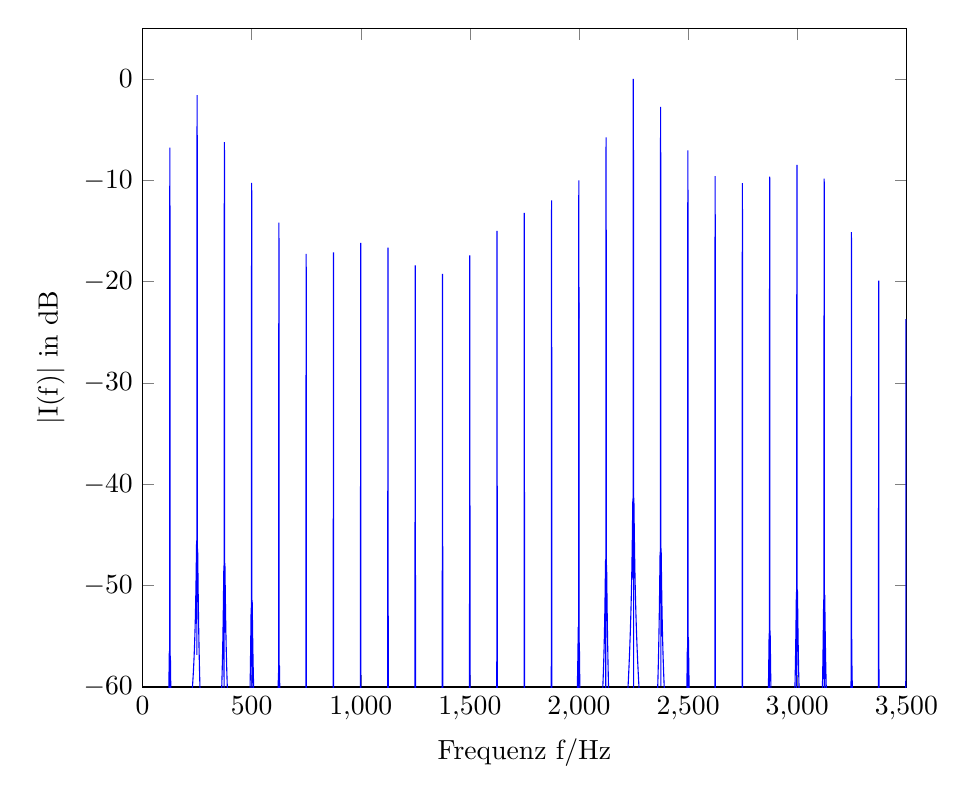
\begin{tikzpicture}

\begin{axis}[%
width=0.8\columnwidth,
%height=0.5\columnwidth,
at={(0\textwidth,0\textwidth)},
scale only axis,
xmin=0,
xmax=3500,
xlabel={Frequenz f/Hz},
ymin=-60,
ymax=5,
ylabel={$|$I(f)$|$ in dB}
]
\addplot [color=blue,solid,forget plot]
  table[row sep=crcr]{%
-0.25	-94.4383425739265\\
0.25	-94.4425033029385\\
0.75	-94.4383425739265\\
1.25	-94.4258832392265\\
1.75	-94.4051934297753\\
2.25	-94.3763852935261\\
2.75	-94.3396129469626\\
3.25	-94.2950697172175\\
3.75	-94.2429847762108\\
4.25	-94.1836192859788\\
4.75	-94.1172621849195\\
5.25	-94.0442257484504\\
5.75	-93.9648410544102\\
6.25	-93.8794534747979\\
6.75	-93.7884183018958\\
7.25	-93.6920966003666\\
7.75	-93.5908513582826\\
8.25	-93.4850439911707\\
8.75	-93.3750312347523\\
9.25	-93.2611624449228\\
9.75	-93.1437773088547\\
10.25	-93.0232039583279\\
10.75	-92.8997574666384\\
11.25	-92.7737387028679\\
11.75	-92.6454335122139\\
12.25	-92.5151121880467\\
12.75	-92.383029200035\\
13.25	-92.2494231428284\\
13.75	-92.1145168710049\\
14.25	-91.9785177880281\\
14.75	-91.8416182595001\\
15.25	-91.7039961239045\\
15.75	-91.5658152770468\\
16.25	-91.4272263094388\\
16.75	-91.2883671787606\\
17.25	-91.149363902324\\
17.75	-91.0103312569967\\
18.25	-90.8713734762511\\
18.75	-90.7325849361451\\
19.25	-90.5940508237426\\
19.75	-90.4558477830128\\
20.25	-90.3180445346328\\
20.75	-90.1807024670676\\
21.25	-90.0438761974301\\
21.75	-89.9076141011551\\
22.25	-89.7719588102729\\
22.75	-89.6369476805002\\
23.25	-89.5026132277323\\
23.75	-89.3689835348366\\
24.25	-89.236082629833\\
24.75	-89.1039308367016\\
25.25	-88.9725451001778\\
25.75	-88.8419392859176\\
26.25	-88.7121244574723\\
26.75	-88.5831091314853\\
27.25	-88.4548995125337\\
27.75	-88.3274997089516\\
28.25	-88.2009119309903\\
28.75	-88.0751366725456\\
29.25	-87.9501728776719\\
29.75	-87.826018093033\\
30.25	-87.7026686073376\\
30.75	-87.5801195787369\\
31.25	-87.4583651512676\\
31.75	-87.3373985610097\\
32.25	-87.2172122329471\\
32.75	-87.0977978692089\\
33.25	-86.9791465294055\\
33.75	-86.8612487037339\\
34.25	-86.7440943794198\\
34.75	-86.6276731010733\\
35.25	-86.5119740254596\\
35.75	-86.3969859711528\\
36.25	-86.2826974635044\\
36.75	-86.1690967753398\\
37.25	-86.0561719637033\\
37.75	-85.9439109030417\\
38.25	-85.8323013150887\\
38.75	-85.7213307957508\\
39.25	-85.6109868392373\\
39.75	-85.5012568596967\\
40.25	-85.3921282105336\\
40.75	-85.2835882016459\\
41.25	-85.1756241147239\\
41.75	-85.0682232168045\\
42.25	-84.9613727722136\\
42.75	-84.8550600530451\\
43.25	-84.7492723482828\\
43.75	-84.6439969717126\\
44.25	-84.5392212686963\\
44.75	-84.4349326219075\\
45.25	-84.3311184561501\\
45.75	-84.2277662422873\\
46.25	-84.1248635003919\\
46.75	-84.0223978021664\\
47.25	-83.9203567726933\\
47.75	-83.8187280915774\\
48.25	-83.717499493522\\
48.75	-83.6166587683871\\
49.25	-83.5161937607651\\
49.75	-83.4160923691227\\
50.25	-83.3163425445216\\
50.75	-83.2169322889751\\
51.25	-83.1178496534351\\
51.75	-83.0190827354697\\
52.25	-82.920619676613\\
52.75	-82.8224486594444\\
53.25	-82.7245579043847\\
53.75	-82.6269356662448\\
54.25	-82.5295702305215\\
54.75	-82.4324499094735\\
55.25	-82.3355630379573\\
55.75	-82.2388979690648\\
56.25	-82.1424430695472\\
56.75	-82.0461867150292\\
57.25	-81.950117285034\\
57.75	-81.8542231578082\\
58.25	-81.7584927049476\\
58.75	-81.6629142858359\\
59.25	-81.5674762418872\\
59.75	-81.4721668905807\\
60.25	-81.3769745193171\\
60.75	-81.2818873790532\\
61.25	-81.1868936777362\\
61.75	-81.0919815735244\\
62.25	-80.9971391677985\\
62.75	-80.902354497899\\
63.25	-80.8076155297586\\
63.75	-80.7129101500472\\
64.25	-80.6182261583542\\
64.75	-80.5235512588802\\
65.25	-80.4288730519505\\
65.75	-80.334179025218\\
66.25	-80.2394565445534\\
66.75	-80.1446928446227\\
67.25	-80.0498750190965\\
67.75	-79.9549900105518\\
68.25	-79.8600245999462\\
68.75	-79.7649653957218\\
69.25	-79.6697988224825\\
69.75	-79.5745111092178\\
70.25	-79.4790882770721\\
70.75	-79.383516126602\\
71.25	-79.2877802245111\\
71.75	-79.191865889831\\
72.25	-79.0957581795031\\
72.75	-78.999441873338\\
73.25	-78.9029014583089\\
73.75	-78.8061211121334\\
74.25	-78.709084686115\\
74.75	-78.611775687176\\
75.25	-78.5141772590536\\
75.75	-78.4162721625904\\
76.25	-78.3180427550687\\
76.75	-78.2194709685259\\
77.25	-78.1205382869837\\
77.75	-78.0212257225254\\
78.25	-77.9215137901345\\
78.75	-77.8213824812288\\
79.25	-77.720811235786\\
79.75	-77.6197789129769\\
80.25	-77.5182637602049\\
80.75	-77.4162433804314\\
81.25	-77.3136946976841\\
81.75	-77.2105939206095\\
82.25	-77.1069165039293\\
82.75	-77.0026371076799\\
83.25	-76.8977295540246\\
83.75	-76.7921667815098\\
84.25	-76.6859207965557\\
84.75	-76.5789626219783\\
85.25	-76.4712622423214\\
85.75	-76.3627885457602\\
86.25	-76.2535092623116\\
86.75	-76.1433908980601\\
87.25	-76.0323986651014\\
87.75	-75.920496406847\\
88.25	-75.8076465183313\\
88.75	-75.6938098611108\\
89.25	-75.5789456723072\\
89.75	-75.4630114673185\\
90.25	-75.3459629356511\\
90.75	-75.2277538292971\\
91.25	-75.1083358430059\\
91.75	-74.9876584857428\\
92.25	-74.8656689425512\\
92.75	-74.7423119259545\\
93.25	-74.6175295159414\\
93.75	-74.4912609874767\\
94.25	-74.3634426243697\\
94.75	-74.2340075181882\\
95.25	-74.1028853507837\\
95.75	-73.9700021588003\\
96.25	-73.8352800783815\\
96.75	-73.6986370680505\\
97.25	-73.5599866075268\\
97.75	-73.4192373699409\\
98.25	-73.2762928646181\\
98.75	-73.1310510472349\\
99.25	-72.9834038937425\\
99.75	-72.8332369339895\\
100.25	-72.6804287404262\\
100.75	-72.5248503666597\\
101.25	-72.3663647298944\\
101.75	-72.2048259304744\\
102.25	-72.0400785007565\\
102.75	-71.8719565744193\\
103.25	-71.7002829659861\\
103.75	-71.5248681487909\\
104.25	-71.3455091177964\\
104.75	-71.1619881215086\\
105.25	-70.9740712447131\\
105.75	-70.7815068207288\\
106.25	-70.5840236482888\\
106.75	-70.3813289838869\\
107.25	-70.1731062752927\\
107.75	-69.9590125957895\\
108.25	-69.7386757312682\\
108.75	-69.5116908633485\\
109.25	-69.2776167808313\\
109.75	-69.0359715385841\\
110.25	-68.7862274668773\\
110.75	-68.5278054145597\\
111.25	-68.2600680854942\\
111.75	-67.9823122983993\\
112.25	-67.6937599645656\\
112.75	-67.3935475346444\\
113.25	-67.0807136136858\\
113.75	-66.7541843820672\\
114.25	-66.4127563892415\\
114.75	-66.0550762102468\\
115.25	-65.6796163801776\\
115.75	-65.2846469696401\\
116.25	-64.8682021794001\\
116.75	-64.4280415107801\\
117.25	-63.9616056130547\\
117.75	-63.4659682540297\\
118.25	-62.9377889483646\\
118.75	-62.3732777174692\\
119.25	-61.7681991302678\\
119.75	-61.1179790564134\\
120.25	-60.4180650502653\\
120.75	-59.6649149020051\\
121.25	-58.8586065807823\\
121.75	-58.0099686951319\\
122.25	-57.1619518017708\\
122.75	-56.4654790009217\\
123.25	-56.5496587111119\\
123.75	-62.9143249259129\\
124.25	-43.3688731539547\\
124.75	-11.9900222001443\\
125.25	-6.78271294059886\\
125.75	-16.5578137201217\\
126.25	-51.3248574230745\\
126.75	-59.8628531891147\\
127.25	-56.9325964375803\\
127.75	-57.2273390533597\\
128.25	-58.0518960326566\\
128.75	-58.9762518635147\\
129.25	-59.8881698175795\\
129.75	-60.7547363864306\\
130.25	-61.5678592073149\\
130.75	-62.327983440334\\
131.25	-63.0384524311005\\
131.75	-63.7033907905205\\
132.25	-64.3268892240077\\
132.75	-64.9127052836891\\
133.25	-65.4641762125291\\
133.75	-65.9842189607838\\
134.25	-66.4753639789448\\
134.75	-66.9397995958508\\
135.25	-67.379417046435\\
135.75	-67.7958521642178\\
136.25	-68.1905224362096\\
136.75	-68.5646593004219\\
137.25	-68.9193360509473\\
137.75	-69.2554918765388\\
138.25	-69.5739525731561\\
138.75	-69.8754484239236\\
139.25	-70.1606296717466\\
139.75	-70.4300799392207\\
140.25	-70.6843278856686\\
140.75	-70.9238573352597\\
141.25	-71.1491160638588\\
141.75	-71.3605233951092\\
142.25	-71.5584767273257\\
142.75	-71.7433570910305\\
143.25	-71.9155338212601\\
143.75	-72.0753684180715\\
144.25	-72.2232176619214\\
144.75	-72.3594360468542\\
145.25	-72.4843775928184\\
145.75	-72.5983970981648\\
146.25	-72.7018508937457\\
146.75	-72.7950971605043\\
147.25	-72.8784958725253\\
147.75	-72.9524084269169\\
148.25	-73.0171970204034\\
148.75	-73.0732238300317\\
149.25	-73.1208500519879\\
149.75	-73.1604348482162\\
150.25	-73.1923342455695\\
150.75	-73.2169000267216\\
151.25	-73.2344786463015\\
151.75	-73.2454101998466\\
152.25	-73.2500274674391\\
152.75	-73.2486550484229\\
153.25	-73.2416085985689\\
153.75	-73.2291941765185\\
154.25	-73.2117077024088\\
154.75	-73.1894345282242\\
155.25	-73.1626491166986\\
155.75	-73.131614823433\\
156.25	-73.0965837752905\\
156.75	-73.0577968369981\\
157.25	-73.0154836571928\\
157.75	-72.9698627848135\\
158.25	-72.9211418466983\\
158.75	-72.8695177774547\\
159.25	-72.8151770930464\\
159.75	-72.7582962000632\\
160.25	-72.6990417332482\\
160.75	-72.6375709145107\\
161.25	-72.5740319273553\\
161.75	-72.5085643013298\\
162.25	-72.4412993017783\\
162.75	-72.3723603208223\\
163.25	-72.3018632660958\\
163.75	-72.2299169443132\\
164.25	-72.1566234372612\\
164.75	-72.0820784682566\\
165.25	-72.0063717575235\\
165.75	-71.9295873652963\\
166.25	-71.8518040217715\\
166.75	-71.7730954433004\\
167.25	-71.6935306344427\\
167.75	-71.6131741757018\\
168.25	-71.5320864969167\\
168.75	-71.4503241364316\\
169.25	-71.3679399862617\\
169.75	-71.284983523572\\
170.25	-71.2015010288457\\
170.75	-71.117535791178\\
171.25	-71.0331283011613\\
171.75	-70.9483164318636\\
172.25	-70.8631356084101\\
172.75	-70.7776189666889\\
173.25	-70.6917975017043\\
173.75	-70.6057002060956\\
174.25	-70.5193541993285\\
174.75	-70.4327848480592\\
175.25	-70.3460158781502\\
175.75	-70.2590694788043\\
176.25	-70.1719663992643\\
176.75	-70.0847260385037\\
177.25	-69.9973665283191\\
177.75	-69.9099048102078\\
178.25	-69.8223567064011\\
178.75	-69.7347369854016\\
179.25	-69.647059422348\\
179.75	-69.559336854524\\
180.25	-69.4715812322941\\
180.75	-69.383803665748\\
181.25	-69.2960144673042\\
181.75	-69.2082231905159\\
182.25	-69.1204386653065\\
182.75	-69.032669029842\\
183.25	-68.9449217592407\\
183.75	-68.8572036913045\\
184.25	-68.7695210494422\\
184.75	-68.6818794629493\\
185.25	-68.5942839847919\\
185.75	-68.5067391070367\\
186.25	-68.4192487740584\\
186.75	-68.3318163936449\\
187.25	-68.2444448461206\\
187.75	-68.1571364915717\\
188.25	-68.0698931753431\\
188.75	-67.9827162317526\\
189.25	-67.8956064863121\\
189.75	-67.8085642563489\\
190.25	-67.7215893502149\\
190.75	-67.6346810651116\\
191.25	-67.5478381836024\\
191.75	-67.4610589688753\\
192.25	-67.3743411588022\\
192.75	-67.2876819588621\\
193.25	-67.2010780339562\\
193.75	-67.1145254991713\\
194.25	-67.0280199095262\\
194.75	-66.9415562487325\\
195.25	-66.8551289170081\\
195.75	-66.7687317179645\\
196.25	-66.682357844594\\
196.75	-66.5959998643772\\
197.25	-66.5096497035251\\
197.75	-66.4232986303677\\
198.25	-66.3369372378974\\
198.75	-66.250555425469\\
199.25	-66.1641423796583\\
199.75	-66.0776865542674\\
200.25	-65.991175649474\\
200.75	-65.9045965901012\\
201.25	-65.8179355029921\\
201.75	-65.7311776934584\\
202.25	-65.6443076207731\\
202.75	-65.5573088726651\\
203.25	-65.4701641387708\\
203.75	-65.3828551829898\\
204.25	-65.2953628146804\\
204.75	-65.207666858629\\
205.25	-65.1197461237121\\
205.75	-65.0315783701629\\
206.25	-64.9431402753453\\
206.75	-64.8544073979258\\
207.25	-64.7653541403191\\
207.75	-64.6759537092791\\
208.25	-64.5861780744808\\
208.75	-64.4959979249361\\
209.25	-64.4053826230606\\
209.75	-64.3143001561978\\
210.25	-64.2227170853838\\
210.75	-64.1305984911177\\
211.25	-64.037907915878\\
211.75	-63.9446073031037\\
212.25	-63.8506569323287\\
212.75	-63.7560153501303\\
213.25	-63.6606392965219\\
213.75	-63.5644836263802\\
214.25	-63.4675012254622\\
214.75	-63.3696429205212\\
215.25	-63.2708573829851\\
215.75	-63.1710910256055\\
216.25	-63.0702878914278\\
216.75	-62.9683895343677\\
217.25	-62.8653348906051\\
217.75	-62.7610601399243\\
218.25	-62.6554985560407\\
218.75	-62.5485803448476\\
219.25	-62.4402324694049\\
219.75	-62.3303784603587\\
220.25	-62.2189382103391\\
220.75	-62.1058277507104\\
221.25	-61.9909590088704\\
221.75	-61.8742395440733\\
222.25	-61.7555722595163\\
222.75	-61.6348550881505\\
223.25	-61.5119806493632\\
223.75	-61.3868358733199\\
224.25	-61.2593015893407\\
224.75	-61.129252074209\\
225.25	-60.9965545557689\\
225.75	-60.8610686665309\\
226.25	-60.7226458412766\\
226.75	-60.5811286518059\\
227.25	-60.4363500709778\\
227.75	-60.2881326570485\\
228.25	-60.1362876479582\\
228.75	-59.9806139536372\\
229.25	-59.8208970325397\\
229.75	-59.6569076364156\\
230.25	-59.4884004047298\\
230.75	-59.3151122870506\\
231.25	-59.1367607680495\\
231.75	-58.95304186536\\
232.25	-58.7636278652755\\
232.75	-58.5681647549347\\
233.25	-58.3662693020006\\
233.75	-58.157525723603\\
234.25	-57.9414818750984\\
234.75	-57.7176448755676\\
235.25	-57.485476070338\\
235.75	-57.2443852105122\\
236.25	-56.9937237046581\\
236.75	-56.7327767674726\\
237.25	-56.4607542532322\\
237.75	-56.1767799169441\\
238.25	-55.8798787921287\\
238.75	-55.5689623103452\\
239.25	-55.2428107143598\\
239.75	-54.9000522374883\\
240.25	-54.5391384454906\\
240.75	-54.1583150866394\\
241.25	-53.755587819198\\
241.75	-53.3286823883245\\
242.25	-52.8749994292804\\
242.75	-52.391565558509\\
243.25	-51.8749858220419\\
243.75	-51.321410246101\\
244.25	-50.7265446489849\\
244.75	-50.08577642914\\
245.25	-49.3945846312073\\
245.75	-48.6496582358787\\
246.25	-47.8518608448083\\
246.75	-47.0144209094212\\
247.25	-46.1879584780304\\
247.75	-45.5523144118615\\
248.25	-45.8964380141639\\
248.75	-56.828617095311\\
249.25	-28.7024518956255\\
249.75	-4.70792109373025\\
250.25	-1.60325981275531\\
250.75	-13.9790407008642\\
251.25	-45.2822389364891\\
251.75	-48.3405592230755\\
252.25	-46.3384873877839\\
252.75	-46.7734649651522\\
253.25	-47.6447639486622\\
253.75	-48.5957810285641\\
254.25	-49.5304537574016\\
254.75	-50.4205841736613\\
255.25	-51.259671369388\\
255.75	-52.0487538807132\\
256.25	-52.7914266359981\\
256.75	-53.4919516387272\\
257.25	-54.154527050811\\
257.75	-54.78301959325\\
258.25	-55.380888501059\\
258.75	-55.9511883380299\\
259.25	-56.4966021885573\\
259.75	-57.0194840741314\\
260.25	-57.5219015140131\\
260.75	-58.0056745978901\\
261.25	-58.4724104057403\\
261.75	-58.9235327025507\\
262.25	-59.3603072857651\\
262.75	-59.7838635145045\\
263.25	-60.1952125651478\\
263.75	-60.5952629160888\\
264.25	-60.9848335026989\\
264.75	-61.3646649189523\\
265.25	-61.7354289822635\\
265.75	-62.0977369255292\\
266.25	-62.4521464356399\\
266.75	-62.7991677202647\\
267.25	-63.139268753682\\
267.75	-63.4728798268173\\
268.25	-63.8003975055874\\
268.75	-64.1221880843239\\
269.25	-64.438590606789\\
269.75	-64.7499195155468\\
270.25	-65.0564669807387\\
270.75	-65.3585049512709\\
271.25	-65.6562869647375\\
271.75	-65.9500497468336\\
272.25	-66.2400146263533\\
272.75	-66.5263887879564\\
273.25	-66.809366381595\\
273.75	-67.0891295047026\\
274.25	-67.3658490708784\\
274.75	-67.6396855767862\\
275.25	-67.9107897772548\\
275.75	-68.1793032770645\\
276.25	-68.4453590466413\\
276.75	-68.7090818677265\\
277.25	-68.9705887141325\\
277.75	-69.229989071817\\
278.25	-69.4873852017508\\
278.75	-69.742872348372\\
279.25	-69.9965388958082\\
279.75	-70.2484664735106\\
280.25	-70.4987300124399\\
280.75	-70.747397752519\\
281.25	-70.9945312016506\\
281.75	-71.2401850462627\\
282.25	-71.4844070130218\\
282.75	-71.7272376810991\\
283.25	-71.9687102441546\\
283.75	-72.2088502210529\\
284.25	-72.4476751142267\\
284.75	-72.6851940145944\\
285.25	-72.9214071520142\\
285.75	-73.1563053904459\\
286.25	-73.3898696673102\\
286.75	-73.6220703770176\\
287.25	-73.8528666993026\\
287.75	-74.0822058738813\\
288.25	-74.3100224241096\\
288.75	-74.5362373337459\\
289.25	-74.7607571827191\\
289.75	-74.9834732499641\\
290.25	-75.2042605939782\\
290.75	-75.4229771247924\\
291.25	-75.6394626845712\\
291.75	-75.8535381580601\\
292.25	-76.0650046385432\\
292.75	-76.273642679847\\
293.25	-76.4792116700634\\
293.75	-76.6814493679667\\
294.25	-76.8800716482646\\
294.75	-77.0747725066391\\
295.25	-77.2652243794297\\
295.75	-77.4510788355387\\
296.25	-77.6319676988497\\
296.75	-77.8075046577428\\
297.25	-77.9772874133488\\
297.75	-78.1409004094275\\
298.25	-78.297918173672\\
298.75	-78.4479092824171\\
299.25	-78.5904409381747\\
299.75	-78.7250841224657\\
300.25	-78.8514192558939\\
300.75	-78.9690422646818\\
301.25	-79.0775709199628\\
301.75	-79.176651285295\\
302.25	-79.2659640818832\\
302.75	-79.3452307628125\\
303.25	-79.414219079307\\
303.75	-79.4727479262412\\
304.25	-79.5206912712405\\
304.75	-79.5579810020382\\
305.25	-79.5846085687295\\
305.75	-79.600625348576\\
306.25	-79.6061417175111\\
306.75	-79.6013248701404\\
307.25	-79.5863954845855\\
307.75	-79.561623375818\\
308.25	-79.5273223181234\\
308.75	-79.4838442417903\\
309.25	-79.4315730203626\\
309.75	-79.3709180631399\\
310.25	-79.3023079146342\\
310.75	-79.2261840405934\\
311.25	-79.1429949517295\\
311.75	-79.0531907841903\\
312.25	-78.9572184226933\\
312.75	-78.8555172203075\\
313.25	-78.7485153398883\\
313.75	-78.6366267169595\\
314.25	-78.5202486236725\\
314.75	-78.3997597975477\\
315.25	-78.2755190878222\\
315.75	-78.147864565194\\
316.25	-78.0171130373766\\
316.75	-77.8835599123586\\
317.25	-77.7474793529642\\
317.75	-77.6091246696463\\
318.25	-77.4687289028159\\
318.75	-77.3265055510599\\
319.25	-77.1826494068519\\
319.75	-77.0373374666516\\
320.25	-76.8907298873281\\
320.75	-76.74297096555\\
321.25	-76.5941901210761\\
321.75	-76.4445028686669\\
322.25	-76.2940117666909\\
322.75	-76.1428073333516\\
323.25	-75.990968923891\\
323.75	-75.8385655641528\\
324.25	-75.6856567375775\\
324.75	-75.5322931239923\\
325.25	-75.3785172897358\\
325.75	-75.2243643293921\\
326.25	-75.0698624601322\\
326.75	-74.9150335701051\\
327.25	-74.7598937226582\\
327.75	-74.6044536184281\\
328.25	-74.4487190174419\\
328.75	-74.2926911234765\\
329.25	-74.1363669329126\\
329.75	-73.9797395503006\\
330.25	-73.8227984727957\\
330.75	-73.6655298455218\\
331.25	-73.5079166898372\\
331.75	-73.3499391063455\\
332.25	-73.1915744543799\\
332.75	-73.0327975095694\\
333.25	-72.8735806009516\\
333.75	-72.7138937289889\\
334.25	-72.5537046657102\\
334.75	-72.392979038078\\
335.25	-72.2316803955695\\
335.75	-72.0697702628404\\
336.25	-71.9072081782288\\
336.75	-71.7439517187567\\
337.25	-71.5799565121723\\
337.75	-71.4151762364853\\
338.25	-71.249562607344\\
338.75	-71.0830653535059\\
339.25	-70.9156321805614\\
339.75	-70.7472087229738\\
340.25	-70.5777384843996\\
340.75	-70.4071627661655\\
341.25	-70.2354205836693\\
341.75	-70.062448570375\\
342.25	-69.8881808689682\\
342.75	-69.7125490091162\\
343.25	-69.535481771169\\
343.75	-69.3569050349972\\
344.25	-69.1767416130352\\
344.75	-68.9949110664341\\
345.25	-68.8113295030725\\
345.75	-68.6259093559822\\
346.25	-68.4385591405438\\
346.75	-68.2491831885764\\
347.25	-68.0576813571908\\
347.75	-67.8639487099803\\
348.25	-67.6678751678019\\
348.75	-67.4693451260189\\
349.25	-67.2682370346561\\
349.75	-67.0644229374284\\
350.25	-66.8577679650414\\
350.75	-66.6481297775217\\
351.25	-66.4353579495881\\
351.75	-66.2192932922085\\
352.25	-65.9997671024876\\
352.75	-65.7766003328624\\
353.25	-65.54960266921\\
353.75	-65.3185715058784\\
354.25	-65.0832908037582\\
354.75	-64.8435298153008\\
355.25	-64.5990416577518\\
355.75	-64.349561712756\\
356.25	-64.0948058267734\\
356.75	-63.8344682823152\\
357.25	-63.5682195046981\\
357.75	-63.2957034626362\\
358.25	-63.0165347133017\\
358.75	-62.7302950331965\\
359.25	-62.4365295649184\\
359.75	-62.1347423962338\\
360.25	-61.824391471229\\
360.75	-61.5048827130434\\
361.25	-61.175563212983\\
361.75	-60.8357133107493\\
362.25	-60.4845373540567\\
362.75	-60.1211528819991\\
363.25	-59.7445779243071\\
363.75	-59.3537160479052\\
364.25	-58.9473387143497\\
364.75	-58.5240644417735\\
365.25	-58.0823342053557\\
365.75	-57.6203824890355\\
366.25	-57.1362034780282\\
366.75	-56.627512182609\\
367.25	-56.0917010737548\\
367.75	-55.5257946558795\\
368.25	-54.9264085332471\\
368.75	-54.289728715573\\
369.25	-53.6115476431534\\
369.75	-52.8874416800642\\
370.25	-52.1132926047389\\
370.75	-51.2866622965009\\
371.25	-50.4104011829712\\
371.75	-49.5026593408774\\
372.25	-48.6280259927394\\
372.75	-48.0162572676959\\
373.25	-48.7418178920483\\
373.75	-71.5508017105879\\
374.25	-26.4854953440571\\
374.75	-7.30352868019295\\
375.25	-6.23079727509385\\
375.75	-21.6081654119154\\
376.25	-54.6326273600718\\
376.75	-48.9919455364187\\
377.25	-47.7819229797393\\
377.75	-48.2928589502265\\
378.25	-49.1279551122924\\
378.75	-50.0108623034038\\
379.25	-50.8657882423304\\
379.75	-51.6712995465898\\
380.25	-52.4235407607879\\
380.75	-53.1246914977364\\
381.25	-53.7788684556959\\
381.75	-54.3905781493179\\
382.25	-54.9641314970626\\
382.75	-55.5034427347355\\
383.25	-56.0119854851453\\
383.75	-56.4928117342359\\
384.25	-56.9485934047576\\
384.75	-57.3816692060564\\
385.25	-57.7940895596537\\
385.75	-58.1876569269737\\
386.25	-58.5639608787489\\
386.75	-58.9244081059633\\
387.25	-59.2702479001623\\
387.75	-59.6025937160642\\
388.25	-59.9224414084558\\
388.75	-60.2306846730887\\
389.25	-60.5281281478242\\
389.75	-60.8154985589896\\
390.25	-61.0934542341266\\
390.75	-61.3625932475211\\
391.25	-61.6234604188917\\
391.75	-61.8765533474566\\
392.25	-62.122327632173\\
392.75	-62.36120140316\\
393.25	-62.5935592681815\\
393.75	-62.8197557607379\\
394.25	-63.0401183620948\\
394.75	-63.2549501578809\\
395.25	-63.4645321802427\\
395.75	-63.6691254785745\\
396.25	-63.8689729552331\\
396.75	-64.0643009971528\\
397.25	-64.2553209296917\\
397.75	-64.4422303152072\\
398.25	-64.6252141156392\\
398.75	-64.8044457356717\\
399.25	-64.9800879607502\\
399.75	-65.1522938023032\\
400.25	-65.3212072608621\\
400.75	-65.4869640163736\\
401.25	-65.6496920538041\\
401.75	-65.8095122311029\\
402.25	-65.9665387957163\\
402.75	-66.1208798550792\\
403.25	-66.2726378058607\\
403.75	-66.4219097261693\\
404.25	-66.5687877344312\\
404.75	-66.7133593182325\\
405.25	-66.8557076360331\\
405.75	-66.9959117943455\\
406.25	-67.1340471026769\\
406.75	-67.2701853082897\\
407.25	-67.4043948126105\\
407.75	-67.5367408709275\\
408.25	-67.6672857768431\\
408.75	-67.7960890327962\\
409.25	-67.9232075078392\\
409.75	-68.0486955837298\\
410.25	-68.1726052902966\\
410.75	-68.2949864309396\\
411.25	-68.4158866990458\\
411.75	-68.5353517860216\\
412.25	-68.6534254815802\\
412.75	-68.7701497668554\\
413.25	-68.8855649008667\\
413.75	-68.9997095008055\\
414.25	-69.1126206165683\\
414.75	-69.2243337999287\\
415.25	-69.3348831686941\\
415.75	-69.4443014661698\\
416.25	-69.5526201162149\\
416.75	-69.6598692741542\\
417.25	-69.7660778737798\\
417.75	-69.8712736706554\\
418.25	-69.9754832819163\\
418.75	-70.078732222737\\
419.25	-70.1810449396215\\
419.75	-70.2824448406513\\
420.25	-70.3829543228225\\
420.75	-70.4825947965668\\
421.25	-70.5813867075644\\
421.75	-70.6793495559239\\
422.25	-70.7765019128017\\
422.75	-70.87286143452\\
423.25	-70.9684448742341\\
423.75	-71.0632680911849\\
424.25	-71.1573460575688\\
424.75	-71.2506928630437\\
425.25	-71.3433217168822\\
425.75	-71.4352449477779\\
426.25	-71.5264740012964\\
426.75	-71.6170194349594\\
427.25	-71.7068909109445\\
427.75	-71.7960971863676\\
428.25	-71.8846461011198\\
428.75	-71.9725445632136\\
429.25	-72.0597985315908\\
429.75	-72.1464129963424\\
430.25	-72.2323919562758\\
430.75	-72.3177383937689\\
431.25	-72.4024542468388\\
431.75	-72.4865403783515\\
432.25	-72.5699965422937\\
432.75	-72.6528213470256\\
433.25	-72.7350122154305\\
433.75	-72.8165653418717\\
434.25	-72.8974756458758\\
434.75	-72.977736722448\\
435.25	-73.0573407889372\\
435.75	-73.1362786283733\\
436.25	-73.214539529188\\
436.75	-73.2921112212555\\
437.25	-73.368979808187\\
437.75	-73.4451296958472\\
438.25	-73.5205435169837\\
438.75	-73.595202052089\\
439.25	-73.6690841463242\\
439.75	-73.7421666226685\\
440.25	-73.8144241912755\\
440.75	-73.8858293551502\\
441.25	-73.9563523122647\\
441.75	-74.0259608542948\\
442.25	-74.0946202621923\\
442.75	-74.1622931988807\\
443.25	-74.2289395994218\\
443.75	-74.2945165590711\\
444.25	-74.35897821973\\
444.75	-74.4222756553807\\
445.25	-74.4843567572004\\
445.75	-74.5451661191504\\
446.25	-74.6046449249523\\
446.75	-74.6627308374951\\
447.25	-74.7193578918366\\
447.75	-74.774456393112\\
448.25	-74.8279528208033\\
448.75	-74.8797697409683\\
449.25	-74.9298257281761\\
449.75	-74.9780352990594\\
450.25	-75.0243088595127\\
450.75	-75.0685526677192\\
451.25	-75.1106688153077\\
451.75	-75.1505552290398\\
452.25	-75.1881056954993\\
452.75	-75.2232099113223\\
453.25	-75.2557535614901\\
453.75	-75.2856184281847\\
454.25	-75.3126825326002\\
454.75	-75.3368203119609\\
455.25	-75.3579028337532\\
455.75	-75.3757980488879\\
456.25	-75.3903710851207\\
456.75	-75.4014845815708\\
457.25	-75.4089990646406\\
457.75	-75.4127733649554\\
458.25	-75.412665074232\\
458.75	-75.4085310401506\\
459.25	-75.4002278964311\\
459.75	-75.3876126243768\\
460.25	-75.3705431411836\\
460.75	-75.3488789093349\\
461.25	-75.3224815604556\\
461.75	-75.2912155260787\\
462.25	-75.2549486669707\\
462.75	-75.2135528919428\\
463.25	-75.1669047565166\\
463.75	-75.114886031438\\
464.25	-75.0573842308468\\
464.75	-74.9942930899659\\
465.25	-74.9255129824546\\
465.75	-74.8509512680983\\
466.25	-74.7705225622774\\
466.75	-74.6841489196411\\
467.25	-74.5917599255947\\
467.75	-74.4932926905599\\
468.25	-74.3886917434263\\
468.75	-74.2779088221542\\
469.25	-74.1609025610395\\
469.75	-74.0376380756676\\
470.25	-73.9080864480147\\
470.75	-73.77222411543\\
471.25	-73.6300321683409\\
471.75	-73.4814955623924\\
472.25	-73.3266022513322\\
472.75	-73.1653422473303\\
473.25	-72.9977066154367\\
473.75	-72.8236864086712\\
474.25	-72.6432715496919\\
474.75	-72.4564496642181\\
475.25	-72.263204870292\\
475.75	-72.0635165261837\\
476.25	-71.8573579381978\\
476.75	-71.6446950279144\\
477.25	-71.4254849564392\\
477.75	-71.1996747011159\\
478.25	-70.9671995778106\\
478.75	-70.7279816993329\\
479.25	-70.4819283577708\\
479.75	-70.2289303154424\\
480.25	-69.9688599857729\\
480.75	-69.7015694815701\\
481.25	-69.426888503843\\
481.75	-69.1446220393239\\
482.25	-68.8545478290698\\
482.75	-68.5564135637328\\
483.25	-68.2499337530537\\
483.75	-67.9347862075433\\
484.25	-67.6106080588015\\
484.75	-67.2769912310241\\
485.25	-66.9334772594055\\
485.75	-66.5795513306962\\
486.25	-66.2146353963242\\
486.75	-65.838080178333\\
487.25	-65.4491558519498\\
487.75	-65.0470411449418\\
488.25	-64.6308105423971\\
488.75	-64.1994192263917\\
489.25	-63.7516853153343\\
489.75	-63.2862689039939\\
490.25	-62.801647357412\\
490.75	-62.2960863130442\\
491.25	-61.7676059651717\\
491.75	-61.2139425891681\\
492.25	-60.6325062155495\\
492.75	-60.0203375343397\\
493.25	-59.3740719167369\\
493.75	-58.6899290815232\\
494.25	-57.9637709358969\\
494.75	-57.1913261680641\\
495.25	-56.3688177990566\\
495.75	-55.4945917990107\\
496.25	-54.573387973492\\
496.75	-53.6283019092966\\
497.25	-52.7387965448757\\
497.75	-52.1918427729062\\
498.25	-53.4398779610317\\
498.75	-57.9797554383091\\
499.25	-25.8014621644716\\
499.75	-10.257832348695\\
500.25	-11.2004747246728\\
500.75	-30.1860753718157\\
501.25	-76.7764976502099\\
501.75	-52.1473958245962\\
502.25	-51.4411349384824\\
502.75	-52.0136540176984\\
503.25	-52.8328877572577\\
503.75	-53.6781518629163\\
504.25	-54.4881238735288\\
504.75	-55.2461591895401\\
505.25	-55.9502107713451\\
505.75	-56.6031893773357\\
506.25	-57.2095112560848\\
506.75	-57.7737979001557\\
507.25	-58.3003934838252\\
507.75	-58.7932092285477\\
508.25	-59.2557003662053\\
508.75	-59.6908949158975\\
509.25	-60.1014398443262\\
509.75	-60.489649985283\\
510.25	-60.8575538037311\\
510.75	-61.206933961857\\
511.25	-61.5393623424219\\
511.75	-61.8562298888049\\
512.25	-62.1587718699058\\
512.75	-62.4480892224109\\
513.25	-62.725166580854\\
513.75	-62.9908875327107\\
514.25	-63.2460475567442\\
514.75	-63.4913650288292\\
515.25	-63.7274906144904\\
515.75	-63.9550153121807\\
516.25	-64.1744773652844\\
516.75	-64.3863682228339\\
517.25	-64.5911376977422\\
517.75	-64.7891984458256\\
518.25	-64.9809298680014\\
518.75	-65.1666815209452\\
519.25	-65.3467761074642\\
519.75	-65.5215121063186\\
520.25	-65.6911660917219\\
520.75	-65.8559947849044\\
521.25	-66.0162368736159\\
521.75	-66.1721146300347\\
522.25	-66.3238353530434\\
522.75	-66.4715926570447\\
523.25	-66.6155676263435\\
523.75	-66.755929851427\\
524.25	-66.8928383612456\\
524.75	-67.0264424636757\\
525.25	-67.1568825047269\\
525.75	-67.2842905556774\\
526.25	-67.4087910361354\\
526.75	-67.5305012800205\\
527.25	-67.649532050582\\
527.75	-67.7659880098296\\
528.25	-67.8799681471008\\
528.75	-67.9915661709328\\
529.25	-68.1008708679199\\
529.75	-68.207966431815\\
530.25	-68.3129327657688\\
530.75	-68.4158457602723\\
531.25	-68.5167775490941\\
531.75	-68.6157967452537\\
532.25	-68.7129686588519\\
532.75	-68.8083554983953\\
533.25	-68.902016557076\\
533.75	-68.9940083853227\\
534.25	-69.0843849508069\\
534.75	-69.1731977869679\\
535.25	-69.2604961310213\\
535.75	-69.3463270523148\\
536.25	-69.4307355718213\\
536.75	-69.5137647734805\\
537.25	-69.595455908034\\
537.75	-69.6758484899392\\
538.25	-69.7549803878994\\
538.75	-69.8328879094921\\
539.25	-69.9096058803409\\
539.75	-69.9851677182311\\
540.25	-70.0596055025435\\
540.75	-70.1329500393397\\
541.25	-70.2052309224077\\
541.75	-70.2764765905545\\
542.25	-70.3467143814002\\
542.75	-70.4159705819156\\
543.25	-70.4842704759194\\
543.75	-70.5516383887379\\
544.25	-70.6180977292111\\
544.75	-70.6836710292127\\
545.25	-70.7483799808493\\
545.75	-70.8122454714708\\
546.25	-70.8752876166351\\
546.75	-70.9375257911448\\
547.25	-70.9989786582712\\
547.75	-71.0596641972673\\
548.25	-71.1195997292701\\
548.75	-71.1788019416768\\
549.25	-71.2372869110791\\
549.75	-71.295070124832\\
550.25	-71.352166501321\\
550.75	-71.4085904090016\\
551.25	-71.4643556842596\\
551.75	-71.5194756481532\\
552.25	-71.5739631220804\\
552.75	-71.6278304424269\\
553.25	-71.6810894742223\\
553.75	-71.7337516238532\\
554.25	-71.7858278508624\\
554.75	-71.8373286788651\\
555.25	-71.8882642056092\\
555.75	-71.9386441122059\\
556.25	-71.9884776715497\\
556.75	-72.0377737559475\\
557.25	-72.0865408439715\\
557.75	-72.13478702655\\
558.25	-72.1825200123068\\
558.75	-72.229747132154\\
559.25	-72.276475343147\\
559.75	-72.3227112316033\\
560.25	-72.368461015482\\
560.75	-72.4137305460292\\
561.25	-72.4585253086743\\
561.75	-72.50285042318\\
562.25	-72.5467106430213\\
562.75	-72.5901103540118\\
563.25	-72.633053572099\\
563.75	-72.6755439404051\\
564.25	-72.7175847253892\\
564.75	-72.7591788121827\\
565.25	-72.8003286990329\\
565.75	-72.8410364908353\\
566.25	-72.8813038917165\\
566.75	-72.9211321966347\\
567.25	-72.960522281948\\
567.75	-72.9994745949108\\
568.25	-73.0379891420475\\
568.75	-73.0760654763439\\
569.25	-73.113702683202\\
569.75	-73.1508993650912\\
570.25	-73.1876536248241\\
570.75	-73.2239630473848\\
571.25	-73.2598246802239\\
571.75	-73.2952350119342\\
572.25	-73.330189949209\\
572.75	-73.3646847919843\\
573.25	-73.3987142066475\\
573.75	-73.4322721972014\\
574.25	-73.4653520742498\\
574.75	-73.4979464216636\\
575.25	-73.5300470607931\\
575.75	-73.5616450120509\\
576.25	-73.5927304537067\\
576.75	-73.6232926777078\\
577.25	-73.6533200423266\\
577.75	-73.6827999214324\\
578.25	-73.7117186501563\\
578.75	-73.7400614667139\\
579.25	-73.7678124501259\\
579.75	-73.7949544535681\\
580.25	-73.8214690330502\\
580.75	-73.8473363711203\\
581.25	-73.8725351952559\\
581.75	-73.8970426905928\\
582.25	-73.9208344066121\\
582.75	-73.9438841573867\\
583.25	-73.9661639149656\\
583.75	-73.9876436954427\\
584.25	-74.0082914372415\\
584.75	-74.0280728711063\\
585.25	-74.0469513812788\\
585.75	-74.0648878572987\\
586.25	-74.0818405358509\\
586.75	-74.097764832042\\
587.25	-74.1126131594768\\
587.75	-74.126334738467\\
588.25	-74.1388753916891\\
588.75	-74.150177326582\\
589.25	-74.160178903758\\
589.75	-74.168814390682\\
590.25	-74.1760136998676\\
590.75	-74.1817021108235\\
591.25	-74.1857999749942\\
591.75	-74.1882224029357\\
592.25	-74.1888789329867\\
592.75	-74.187673180723\\
593.25	-74.1845024685087\\
593.75	-74.1792574345142\\
594.25	-74.1718216206228\\
594.75	-74.1620710387251\\
595.25	-74.1498737149769\\
595.75	-74.135089211712\\
596.25	-74.1175681267872\\
596.75	-74.0971515702841\\
597.25	-74.0736706186071\\
597.75	-74.0469457461463\\
598.25	-74.0167862348099\\
598.75	-73.982989561846\\
599.25	-73.9453407664475\\
599.75	-73.9036117956999\\
600.25	-73.8575608304059\\
600.75	-73.8069315912187\\
601.25	-73.7514526252994\\
601.75	-73.6908365733289\\
602.25	-73.6247794161257\\
602.75	-73.5529596992752\\
603.25	-73.4750377330098\\
603.75	-73.3906547630156\\
604.25	-73.2994321057865\\
604.75	-73.2009702395084\\
605.25	-73.0948478381274\\
605.75	-72.9806207320969\\
606.25	-72.8578207741792\\
606.75	-72.7259545824349\\
607.25	-72.5845021250058\\
607.75	-72.432915102248\\
608.25	-72.2706150710199\\
608.75	-72.0969912431725\\
609.25	-71.9113978752403\\
609.75	-71.7131511485913\\
610.25	-71.5015254184498\\
610.75	-71.2757486856836\\
611.25	-71.0349971164071\\
611.75	-70.7783884005615\\
612.25	-70.5049737008449\\
612.75	-70.2137278969277\\
613.25	-69.9035377763592\\
613.75	-69.573187763384\\
614.25	-69.2213427126483\\
614.75	-68.846527233613\\
615.25	-68.4471009700702\\
615.75	-68.0212292737281\\
616.25	-67.5668488577736\\
616.75	-67.0816284555557\\
617.25	-66.5629255774161\\
617.75	-66.0077428744115\\
618.25	-65.4126929581851\\
618.75	-64.7739923696033\\
619.25	-64.087532215278\\
619.75	-63.3491360269224\\
620.25	-62.5552715101746\\
620.75	-61.7048979836748\\
621.25	-60.8043458945534\\
621.75	-59.881175112129\\
622.25	-59.0292636470418\\
622.75	-58.5958896945873\\
623.25	-60.4979391331197\\
623.75	-57.8994831277691\\
624.25	-26.7169588391525\\
624.75	-14.1744427349301\\
625.25	-17.1555924863757\\
625.75	-40.8113789054897\\
626.25	-68.7921014383445\\
626.75	-58.2116963437976\\
627.25	-57.855830341714\\
627.75	-58.4801976088099\\
628.25	-59.2933772601249\\
628.75	-60.1152182154663\\
629.25	-60.8951878868303\\
629.75	-61.6202203582302\\
630.25	-62.2896210986067\\
630.75	-62.9068612080023\\
631.25	-63.4766098965377\\
631.75	-64.0036164943504\\
632.25	-64.4923013417242\\
632.75	-64.9466309670269\\
633.25	-65.3701081088122\\
633.75	-65.7658058623949\\
634.25	-66.1364158181938\\
634.75	-66.48429747468\\
635.25	-66.8115238785333\\
635.75	-67.1199218464004\\
636.25	-67.4111066024593\\
636.75	-67.6865112672826\\
637.25	-67.9474118338043\\
637.75	-68.1949482881151\\
638.25	-68.4301424809399\\
638.75	-68.6539132787569\\
639.25	-68.8670894436751\\
639.75	-69.0704206176775\\
640.25	-69.2645867228335\\
640.75	-69.4502060349955\\
641.25	-69.6278421435383\\
641.75	-69.7980099726751\\
642.25	-69.9611810095301\\
642.75	-70.1177878593308\\
643.25	-70.2682282277723\\
643.75	-70.4128684139968\\
644.25	-70.5520463839891\\
644.75	-70.6860744829952\\
645.25	-70.8152418363256\\
645.75	-70.9398164802707\\
646.25	-71.0600472585191\\
646.75	-71.1761655142002\\
647.25	-71.2883866032682\\
647.75	-71.3969112512596\\
648.25	-71.5019267723565\\
648.75	-71.6036081670778\\
649.25	-71.7021191127059\\
649.75	-71.7976128586862\\
650.25	-71.8902330376377\\
650.75	-71.9801144012494\\
651.25	-72.0673834891743\\
651.75	-72.1521592380257\\
652.25	-72.2345535367213\\
652.75	-72.3146717336745\\
653.25	-72.3926131006855\\
653.75	-72.468471257828\\
654.25	-72.5423345631378\\
654.75	-72.6142864704859\\
655.25	-72.6844058586421\\
655.75	-72.7527673342268\\
656.25	-72.8194415109298\\
656.75	-72.8844952671628\\
657.25	-72.9479919840612\\
657.75	-73.0099917655635\\
658.25	-73.07055164213\\
658.75	-73.1297257594993\\
659.25	-73.187565553745\\
659.75	-73.2441199137817\\
660.25	-73.299435332349\\
660.75	-73.3535560464132\\
661.25	-73.4065241678393\\
661.75	-73.4583798051021\\
662.25	-73.5091611767421\\
662.75	-73.5589047172049\\
663.25	-73.6076451756506\\
663.75	-73.6554157082615\\
664.25	-73.7022479645391\\
664.75	-73.7481721680346\\
665.25	-73.7932171919194\\
665.75	-73.8374106297717\\
666.25	-73.8807788619203\\
666.75	-73.9233471176616\\
667.25	-73.9651395336402\\
667.75	-74.0061792086572\\
668.25	-74.046488255152\\
668.75	-74.0860878475869\\
669.25	-74.1249982679369\\
669.75	-74.1632389484823\\
670.25	-74.2008285120793\\
670.75	-74.2377848100728\\
671.25	-74.2741249580029\\
671.75	-74.3098653692465\\
672.25	-74.3450217867245\\
672.75	-74.3796093127911\\
673.25	-74.4136424374237\\
673.75	-74.4471350648086\\
674.25	-74.4801005384281\\
674.75	-74.5125516647266\\
675.25	-74.5445007354511\\
675.75	-74.5759595487308\\
676.25	-74.6069394289779\\
676.75	-74.6374512456672\\
677.25	-74.6675054310606\\
677.75	-74.697111996936\\
678.25	-74.7262805503646\\
678.75	-74.7550203085984\\
679.25	-74.7833401131025\\
679.75	-74.8112484427822\\
680.25	-74.8387534264425\\
680.75	-74.8658628545121\\
681.25	-74.8925841900739\\
681.75	-74.9189245792261\\
682.25	-74.9448908608077\\
682.75	-74.9704895755107\\
683.25	-74.9957269744088\\
683.75	-75.0206090269189\\
684.25	-75.0451414282229\\
684.75	-75.0693296061608\\
685.25	-75.0931787276196\\
685.75	-75.1166937044266\\
686.25	-75.1398791987669\\
686.75	-75.1627396281313\\
687.25	-75.1852791698047\\
687.75	-75.2075017649229\\
688.25	-75.2294111220557\\
688.75	-75.2510107203988\\
689.25	-75.2723038124999\\
689.75	-75.2932934265784\\
690.25	-75.3139823684109\\
690.75	-75.334373222796\\
691.25	-75.354468354591\\
691.75	-75.3742699093213\\
692.25	-75.393779813354\\
692.75	-75.4129997736329\\
693.25	-75.4319312769679\\
693.75	-75.4505755888656\\
694.25	-75.4689337518949\\
694.75	-75.4870065835702\\
695.25	-75.5047946737401\\
695.75	-75.5222983814651\\
696.25	-75.5395178313605\\
696.75	-75.5564529093899\\
697.25	-75.5731032580791\\
697.75	-75.5894682711282\\
698.25	-75.605547087388\\
698.75	-75.6213385841757\\
699.25	-75.6368413698804\\
699.75	-75.6520537758377\\
700.25	-75.6669738474109\\
700.75	-75.6815993342469\\
701.25	-75.6959276796445\\
701.75	-75.7099560089816\\
702.25	-75.7236811171421\\
702.75	-75.7370994548693\\
703.25	-75.7502071139729\\
703.75	-75.7629998113102\\
704.25	-75.7754728714491\\
704.75	-75.7876212079167\\
705.25	-75.7994393029281\\
705.75	-75.8109211854754\\
706.25	-75.8220604076519\\
706.75	-75.8328500190693\\
707.25	-75.8432825392141\\
707.75	-75.8533499275774\\
708.25	-75.8630435513676\\
708.75	-75.8723541506106\\
709.25	-75.8812718004071\\
709.75	-75.8897858701039\\
710.25	-75.8978849791127\\
710.75	-75.9055569490721\\
711.25	-75.9127887520349\\
711.75	-75.9195664543059\\
712.25	-75.9258751555449\\
712.75	-75.9316989226843\\
713.25	-75.9370207181777\\
713.75	-75.9418223220396\\
714.25	-75.9460842470765\\
714.75	-75.9497856466491\\
715.25	-75.9529042142253\\
715.75	-75.9554160739092\\
716.25	-75.9572956610319\\
716.75	-75.9585155918028\\
717.25	-75.9590465208659\\
717.75	-75.9588569855344\\
718.25	-75.9579132352673\\
718.75	-75.9561790448262\\
719.25	-75.9536155093494\\
719.75	-75.950180819362\\
720.25	-75.9458300135068\\
720.75	-75.9405147065068\\
721.25	-75.9341827895531\\
721.75	-75.9267780999627\\
722.25	-75.9182400565516\\
722.75	-75.9085032567025\\
723.25	-75.8974970305852\\
723.75	-75.8851449473973\\
724.25	-75.8713642677951\\
724.75	-75.8560653359124\\
725.25	-75.8391509034591\\
725.75	-75.8205153773621\\
726.25	-75.8000439812221\\
726.75	-75.7776118194908\\
727.25	-75.7530828316996\\
727.75	-75.7263086222501\\
728.25	-75.6971271491639\\
728.75	-75.6653612527637\\
729.25	-75.6308170024233\\
729.75	-75.5932818362446\\
730.25	-75.5525224647032\\
730.75	-75.5082825048563\\
731.25	-75.4602798065352\\
731.75	-75.4082034258601\\
732.25	-75.3517101943495\\
732.75	-75.2904208235619\\
733.25	-75.2239154754507\\
733.75	-75.1517287170984\\
734.25	-75.0733437649566\\
734.75	-74.9881859076699\\
735.25	-74.8956149776271\\
735.75	-74.7949167188793\\
736.25	-74.685292872447\\
736.75	-74.565849768417\\
737.25	-74.4355851769502\\
737.75	-74.2933731264704\\
738.25	-74.1379463465912\\
738.75	-73.9678759360435\\
739.25	-73.7815477944254\\
739.75	-73.5771352976399\\
740.25	-73.3525676560727\\
740.75	-73.1054934064455\\
741.25	-72.8332386266188\\
741.75	-72.532759884005\\
742.25	-72.2005929665551\\
742.75	-71.8328008238138\\
743.25	-71.4249294699827\\
743.75	-70.9719925572537\\
744.25	-70.4685327507711\\
744.75	-69.9088732876687\\
745.25	-69.2878367841816\\
745.75	-68.6026495445588\\
746.25	-67.8580599346834\\
746.75	-67.0811470191036\\
747.25	-66.3706128012808\\
747.75	-66.1081405951996\\
748.25	-68.5389102759018\\
748.75	-61.7735055747719\\
749.25	-27.2007308333062\\
749.75	-17.270029282604\\
750.25	-22.3536356114644\\
750.75	-53.014849488125\\
751.25	-72.6492887419821\\
751.75	-66.7176671101875\\
752.25	-66.6195265974719\\
752.75	-67.2932839880017\\
753.25	-68.1075033562809\\
753.75	-68.9101404106849\\
754.25	-69.6582672219283\\
754.75	-70.3415885844143\\
755.25	-70.9608054557512\\
755.75	-71.5203602923615\\
756.25	-72.0257590027826\\
756.75	-72.4825402006596\\
757.25	-72.8958867347359\\
757.75	-73.2704997540077\\
758.25	-73.6105817375546\\
758.75	-73.9198634743944\\
759.25	-74.2016467534506\\
759.75	-74.4588504589432\\
760.25	-74.6940548689107\\
760.75	-74.9095421636684\\
761.25	-75.1073325954525\\
761.75	-75.2892164011103\\
762.25	-75.456781792864\\
762.75	-75.6114394418191\\
763.25	-75.7544438712256\\
763.75	-75.8869121469293\\
764.25	-76.0098402120806\\
764.75	-76.1241171714832\\
765.25	-76.230537791962\\
765.75	-76.3298134501871\\
766.25	-76.4225817286904\\
766.75	-76.5094148341683\\
767.25	-76.5908269890695\\
767.75	-76.6672809275192\\
768.25	-76.7391936093827\\
768.75	-76.8069412513492\\
769.25	-76.8708637610001\\
769.75	-76.9312686486387\\
770.25	-76.9884344819434\\
770.75	-77.042613940108\\
771.25	-77.0940365168165\\
771.75	-77.142910915063\\
772.25	-77.1894271713279\\
772.75	-77.2337585418378\\
773.25	-77.2760631794708\\
773.75	-77.3164856262865\\
774.25	-77.3551581434885\\
774.75	-77.392201897923\\
775.25	-77.4277280218339\\
775.75	-77.4618385605165\\
776.25	-77.4946273207348\\
776.75	-77.5261806311764\\
777.25	-77.5565780248621\\
777.75	-77.5858928522279\\
778.25	-77.6141928325642\\
778.75	-77.6415405505688\\
779.25	-77.6679939039893\\
779.75	-77.6936065076268\\
780.25	-77.7184280583508\\
780.75	-77.7425046652705\\
781.25	-77.765879148687\\
781.75	-77.788591311094\\
782.25	-77.8106781830806\\
782.75	-77.8321742467108\\
783.25	-77.8531116386374\\
783.75	-77.8735203349877\\
784.25	-77.8934283198205\\
784.75	-77.9128617387645\\
785.25	-77.9318450392826\\
785.75	-77.9504010988453\\
786.25	-77.9685513421666\\
786.75	-77.9863158485379\\
787.25	-78.0037134501762\\
787.75	-78.0207618224414\\
788.25	-78.0374775666374\\
788.75	-78.0538762861006\\
789.25	-78.0699726561628\\
789.75	-78.0857804885427\\
790.25	-78.101312790655\\
790.75	-78.1165818202882\\
791.25	-78.1315991360429\\
791.75	-78.1463756439048\\
792.25	-78.1609216402817\\
792.75	-78.1752468517925\\
793.25	-78.1893604720923\\
793.75	-78.2032711959755\\
794.25	-78.2169872509732\\
794.75	-78.2305164266641\\
795.25	-78.2438661018675\\
795.75	-78.2570432698984\\
796.25	-78.2700545620348\\
796.75	-78.2829062693373\\
797.25	-78.2956043629501\\
797.75	-78.308154513001\\
798.25	-78.3205621062057\\
798.75	-78.3328322622786\\
799.25	-78.344969849234\\
799.75	-78.3569794976656\\
800.25	-78.3688656140793\\
800.75	-78.3806323933414\\
801.25	-78.3922838303194\\
801.75	-78.4038237307595\\
802.25	-78.4152557214651\\
802.75	-78.4265832598224\\
803.25	-78.4378096427145\\
803.75	-78.4489380148761\\
804.25	-78.459971376714\\
804.75	-78.4709125916471\\
805.25	-78.4817643929747\\
805.75	-78.4925293903297\\
806.25	-78.5032100757253\\
806.75	-78.5138088292304\\
807.25	-78.524327924296\\
807.75	-78.5347695327513\\
808.25	-78.5451357294982\\
808.75	-78.5554284969129\\
809.25	-78.5656497289801\\
809.75	-78.5758012351738\\
810.25	-78.5858847440958\\
810.75	-78.595901906892\\
811.25	-78.6058543004587\\
811.75	-78.6157434304431\\
812.25	-78.6255707340469\\
812.75	-78.6353375827024\\
813.25	-78.6450452844643\\
813.75	-78.6546950863887\\
814.25	-78.6642881766404\\
814.75	-78.6738256865099\\
815.25	-78.6833086922781\\
815.75	-78.6927382169524\\
816.25	-78.7021152318652\\
816.75	-78.7114406581676\\
817.25	-78.7207153681846\\
817.75	-78.7299401866735\\
818.25	-78.7391158919649\\
818.75	-78.7482432169971\\
819.25	-78.7573228502504\\
819.75	-78.7663554365772\\
820.25	-78.7753415779326\\
820.75	-78.7842818340109\\
821.25	-78.7931767227826\\
821.75	-78.8020267209376\\
822.25	-78.8108322642338\\
822.75	-78.8195937477516\\
823.25	-78.8283115260516\\
823.75	-78.8369859132413\\
824.25	-78.8456171829391\\
824.75	-78.8542055681469\\
825.25	-78.8627512610206\\
825.75	-78.8712544125369\\
826.25	-78.8797151320586\\
826.75	-78.8881334867881\\
827.25	-78.8965095011156\\
827.75	-78.9048431558435\\
828.25	-78.9131343872954\\
828.75	-78.9213830862942\\
829.25	-78.9295890970135\\
829.75	-78.9377522156806\\
830.25	-78.9458721891387\\
830.75	-78.9539487132501\\
831.25	-78.9619814311293\\
831.75	-78.9699699312062\\
832.25	-78.9779137450946\\
832.75	-78.9858123452607\\
833.25	-78.9936651424744\\
833.75	-79.0014714830265\\
834.25	-79.0092306456972\\
834.75	-79.0169418384524\\
835.25	-79.0246041948457\\
835.75	-79.032216770111\\
836.25	-79.0397785368993\\
836.75	-79.0472883806558\\
837.25	-79.0547450945801\\
837.75	-79.0621473741517\\
838.25	-79.0694938111639\\
838.75	-79.0767828872397\\
839.25	-79.0840129667626\\
839.75	-79.0911822891682\\
840.25	-79.0982889605498\\
840.75	-79.1053309444907\\
841.25	-79.1123060520474\\
841.75	-79.1192119308088\\
842.25	-79.1260460529152\\
842.75	-79.132805701942\\
843.25	-79.1394879585111\\
843.75	-79.1460896845003\\
844.25	-79.1526075056826\\
844.75	-79.159037792623\\
845.25	-79.165376639624\\
845.75	-79.1716198414892\\
846.25	-79.1777628678485\\
846.75	-79.1838008347298\\
847.25	-79.1897284730475\\
847.75	-79.1955400936068\\
848.25	-79.2012295481721\\
848.75	-79.2067901860826\\
849.25	-79.2122148058073\\
849.75	-79.217495600751\\
850.25	-79.2226240985032\\
850.75	-79.2275910925906\\
851.25	-79.2323865656415\\
851.75	-79.2369996026803\\
852.25	-79.2414182930575\\
852.75	-79.2456296192415\\
853.25	-79.249619330391\\
853.75	-79.2533717982371\\
854.25	-79.256869852329\\
854.75	-79.2600945911548\\
855.25	-79.2630251649159\\
855.75	-79.2656385249176\\
856.25	-79.2679091334742\\
856.75	-79.2698086269213\\
857.25	-79.2713054227357\\
857.75	-79.2723642597197\\
858.25	-79.2729456576893\\
858.75	-79.2730052798906\\
859.25	-79.2724931773092\\
859.75	-79.2713528888317\\
860.25	-79.2695203645398\\
860.75	-79.2669226707924\\
861.25	-79.2634764245012\\
861.75	-79.2590858893218\\
862.25	-79.2536406471015\\
862.75	-79.2470127322865\\
863.25	-79.239053082774\\
863.75	-79.2295871149193\\
864.25	-79.2184091687579\\
864.75	-79.2052754865023\\
865.25	-79.189895275513\\
865.75	-79.1719192573477\\
866.25	-79.1509249076578\\
866.75	-79.1263973421841\\
867.25	-79.0977045135962\\
867.75	-79.0640651177796\\
868.25	-79.0245075844967\\
868.75	-78.9778193890749\\
869.25	-78.9224895041212\\
869.75	-78.8566584013892\\
870.25	-78.7781254221653\\
870.75	-78.68457273082\\
871.25	-78.5745217487448\\
871.75	-78.4508139902185\\
872.25	-78.3336628106253\\
872.75	-78.3171234223037\\
873.25	-78.8957222256552\\
873.75	-82.1139587061058\\
874.25	-24.6925668056371\\
874.75	-17.1287443743368\\
875.25	-24.4194534449436\\
875.75	-75.5113388050455\\
876.25	-80.7582621799239\\
876.75	-81.3018166513556\\
877.25	-81.3011649382001\\
877.75	-81.2101466418242\\
878.25	-81.1085242930479\\
878.75	-81.0152566147216\\
879.25	-80.9343089378962\\
879.75	-80.8653820505179\\
880.25	-80.8070400719458\\
880.75	-80.7576964254878\\
881.25	-80.7159143550386\\
881.75	-80.6804763016965\\
882.25	-80.6503765479891\\
882.75	-80.6247917827736\\
883.25	-80.6030488413658\\
883.75	-80.5845958738992\\
884.25	-80.5689784088165\\
884.75	-80.5558200997572\\
885.25	-80.5448074487484\\
885.75	-80.5356777410367\\
886.25	-80.5282095154601\\
886.75	-80.5222150167607\\
887.25	-80.5175341921926\\
887.75	-80.5140298921668\\
888.25	-80.5115840123079\\
888.75	-80.5100943746182\\
889.25	-80.5094721917622\\
889.75	-80.5096399938058\\
890.25	-80.5105299237574\\
890.75	-80.5120823288115\\
891.25	-80.5142445900092\\
891.75	-80.5169701451466\\
892.25	-80.5202176691521\\
892.75	-80.5239503834214\\
893.25	-80.5281354712903\\
893.75	-80.5327435812766\\
894.25	-80.5377484032252\\
894.75	-80.5431263052919\\
895.25	-80.5488560218967\\
895.75	-80.5549183845638\\
896.25	-80.5612960889794\\
896.75	-80.5679734927639\\
897.25	-80.5749364393672\\
897.75	-80.5821721042841\\
898.25	-80.5896688603735\\
898.75	-80.5974161596156\\
899.25	-80.605404429031\\
899.75	-80.6136249788489\\
900.25	-80.6220699213016\\
900.75	-80.6307320986593\\
901.25	-80.6396050193259\\
901.75	-80.6486828009808\\
902.25	-80.6579601199014\\
902.75	-80.6674321657141\\
903.25	-80.6770946009367\\
903.75	-80.6869435247369\\
904.25	-80.696975440439\\
904.75	-80.7071872263537\\
905.25	-80.7175761095438\\
905.75	-80.7281396422424\\
906.25	-80.7388756806044\\
906.75	-80.7497823655698\\
907.25	-80.7608581056124\\
907.75	-80.7721015611865\\
908.25	-80.7835116307019\\
908.75	-80.7950874378828\\
909.25	-80.806828320372\\
909.75	-80.8187338194754\\
910.25	-80.8308036709347\\
910.75	-80.8430377966421\\
911.25	-80.8554362972113\\
911.75	-80.8679994453419\\
912.25	-80.8807276798992\\
912.75	-80.8936216006742\\
913.25	-80.9066819637384\\
913.75	-80.9199096773924\\
914.25	-80.9333057986294\\
914.75	-80.9468715300984\\
915.25	-80.9606082175347\\
915.75	-80.9745173476225\\
916.25	-80.988600546262\\
916.75	-81.0028595772379\\
917.25	-81.0172963412513\\
917.75	-81.0319128753034\\
918.25	-81.0467113524155\\
918.75	-81.0616940816827\\
919.25	-81.0768635086377\\
919.75	-81.092222215924\\
920.25	-81.1077729242649\\
920.75	-81.1235184937299\\
921.25	-81.1394619252905\\
921.75	-81.1556063626624\\
922.25	-81.171955094434\\
922.75	-81.1885115564776\\
923.25	-81.2052793346514\\
923.75	-81.222262167785\\
924.25	-81.239463950963\\
924.75	-81.2568887390976\\
925.25	-81.2745407508088\\
925.75	-81.292424372612\\
926.25	-81.3105441634191\\
926.75	-81.3289048593759\\
927.25	-81.3475113790154\\
927.75	-81.3663688287862\\
928.25	-81.3854825089178\\
928.75	-81.4048579196756\\
929.25	-81.4245007679995\\
929.75	-81.4444169745534\\
930.25	-81.4646126812004\\
930.75	-81.4850942589231\\
931.25	-81.5058683162164\\
931.75	-81.5269417079679\\
932.25	-81.5483215448603\\
932.75	-81.5700152033149\\
933.25	-81.5920303360178\\
933.75	-81.6143748830497\\
934.25	-81.6370570836567\\
934.75	-81.6600854887069\\
935.25	-81.6834689738674\\
935.75	-81.707216753542\\
936.25	-81.7313383956261\\
936.75	-81.7558438371452\\
937.25	-81.7807434006251\\
937.75	-81.8060478120921\\
938.25	-81.8317682188214\\
938.75	-81.8579162097808\\
939.25	-81.8845038360287\\
939.75	-81.9115436329675\\
940.25	-81.9390486437887\\
940.75	-81.9670324443874\\
941.25	-81.9955091698244\\
941.75	-82.0244935424456\\
942.25	-82.0540009017887\\
942.75	-82.0840472363983\\
943.25	-82.1146492176948\\
943.75	-82.1458242360516\\
944.25	-82.1775904392512\\
944.75	-82.2099667734965\\
945.25	-82.2429730271868\\
945.75	-82.2766298776664\\
946.25	-82.3109589411921\\
946.75	-82.3459828263759\\
947.25	-82.3817251913888\\
947.75	-82.4182108052371\\
948.25	-82.4554656134576\\
948.75	-82.4935168086034\\
949.25	-82.53239290594\\
949.75	-82.5721238247963\\
950.25	-82.6127409760929\\
950.75	-82.6542773565759\\
951.25	-82.6967676503929\\
951.75	-82.7402483386749\\
952.25	-82.7847578178732\\
952.75	-82.8303365276979\\
953.25	-82.8770270895679\\
953.75	-82.9248744566163\\
954.25	-82.9739260763825\\
954.75	-83.0242320674907\\
955.25	-83.0758454117321\\
955.75	-83.128822163159\\
956.25	-83.1832216759966\\
956.75	-83.2391068533821\\
957.25	-83.2965444192108\\
957.75	-83.3556052156658\\
958.25	-83.4163645293178\\
958.75	-83.4789024490865\\
959.25	-83.5433042597924\\
959.75	-83.6096608755325\\
960.25	-83.6780693177188\\
960.75	-83.7486332432879\\
961.25	-83.8214635294079\\
961.75	-83.8966789219384\\
962.25	-83.9744067559847\\
962.75	-84.0547837581894\\
963.25	-84.1379569418989\\
963.75	-84.2240846081488\\
964.25	-84.3133374675384\\
964.75	-84.40589990055\\
965.25	-84.5019713769337\\
965.75	-84.6017680583635\\
966.25	-84.705524612912\\
966.75	-84.8134962751586\\
967.25	-84.925961192106\\
967.75	-85.0432231028433\\
968.25	-85.1656144093873\\
968.75	-85.2934997078511\\
969.25	-85.4272798634724\\
969.75	-85.5673967310518\\
970.25	-85.7143386447061\\
970.75	-85.8686468290496\\
971.25	-86.0309229194527\\
971.75	-86.2018378243158\\
972.25	-86.382142220052\\
972.75	-86.5726790440645\\
973.25	-86.7743984473706\\
973.75	-86.9883757944808\\
974.25	-87.2158334633068\\
974.75	-87.4581674162429\\
975.25	-87.7169798037325\\
975.75	-87.9941192493358\\
976.25	-88.2917309850716\\
976.75	-88.612319703397\\
977.25	-88.9588289248264\\
977.75	-89.334741912387\\
978.25	-89.7442107461236\\
978.75	-90.1922220741096\\
979.25	-90.6848099899734\\
979.75	-91.2293273956894\\
980.25	-91.8347839089673\\
980.75	-92.5122417837435\\
981.25	-93.2752057752017\\
981.75	-94.1397751330551\\
982.25	-95.1238329757924\\
982.75	-96.243107655956\\
983.25	-97.4978276158537\\
983.75	-98.8333940309433\\
984.25	-100.046260373146\\
984.75	-100.676042866941\\
985.25	-100.234756747189\\
985.75	-98.8189452637117\\
986.25	-96.9669523977833\\
986.75	-95.0667847981536\\
987.25	-93.2672883659973\\
987.75	-91.6003450829593\\
988.25	-90.0577629438371\\
988.75	-88.6209854353324\\
989.25	-87.2708065977505\\
989.75	-85.9900649371037\\
990.25	-84.7640399486655\\
990.75	-83.5801638120396\\
991.25	-82.4275837935458\\
991.75	-81.2967436453607\\
992.25	-80.1790294659275\\
992.75	-79.0664890993848\\
993.25	-77.9516317892052\\
993.75	-76.8273330604815\\
994.25	-75.6869161555209\\
994.75	-74.5245901348999\\
995.25	-73.3366969815274\\
995.75	-72.1249664371532\\
996.25	-70.9052764286205\\
996.75	-69.7337167306716\\
997.25	-68.7997059373161\\
997.75	-68.8978029504465\\
998.25	-78.7871674488274\\
998.75	-53.0659253757318\\
999.25	-21.5310504943626\\
999.75	-16.1765113394693\\
1000.25	-25.8300440972391\\
1000.75	-62.1980747190324\\
1001.25	-67.2492340811987\\
1001.75	-64.9153501613617\\
1002.25	-65.1420018806938\\
1002.75	-65.7905195940739\\
1003.25	-66.5042077900835\\
1003.75	-67.1923061687194\\
1004.25	-67.8305867344138\\
1004.75	-68.4151727220438\\
1005.25	-68.9488155555844\\
1005.75	-69.4362354130369\\
1006.25	-69.8824385221431\\
1006.75	-70.2921157922487\\
1007.25	-70.6694574565376\\
1007.75	-71.0181303090574\\
1008.25	-71.3413157912687\\
1008.75	-71.6417670161788\\
1009.25	-71.9218675908421\\
1009.75	-72.1836856601207\\
1010.25	-72.429021135094\\
1010.75	-72.6594459796063\\
1011.25	-72.8763381714493\\
1011.75	-73.0809101813743\\
1012.25	-73.2742328185268\\
1012.75	-73.4572552097043\\
1013.25	-73.6308215727771\\
1013.75	-73.7956853381061\\
1014.25	-73.9525210761356\\
1014.75	-74.1019346075584\\
1015.25	-74.244471604321\\
1015.75	-74.3806249337622\\
1016.25	-74.5108409525821\\
1016.75	-74.635524920286\\
1017.25	-74.7550456717165\\
1017.75	-74.8697396639005\\
1018.25	-74.9799144926307\\
1018.75	-75.0858519580609\\
1019.25	-75.1878107454198\\
1019.75	-75.286028776145\\
1020.25	-75.380725275873\\
1020.75	-75.4721025984036\\
1021.25	-75.5603478387016\\
1021.75	-75.6456342629782\\
1022.25	-75.7281225797187\\
1022.75	-75.8079620720024\\
1023.25	-75.88529160856\\
1023.75	-75.960240548526\\
1024.25	-76.032929552773\\
1024.75	-76.1034713129516\\
1025.25	-76.1719712078679\\
1025.75	-76.2385278955592\\
1026.25	-76.3032338483377\\
1026.75	-76.366175837148\\
1027.25	-76.4274353707875\\
1027.75	-76.4870890948459\\
1028.25	-76.545209154636\\
1028.75	-76.6018635258719\\
1029.25	-76.6571163164046\\
1029.75	-76.7110280419507\\
1030.25	-76.7636558783936\\
1030.75	-76.815053892975\\
1031.25	-76.865273256399\\
1031.75	-76.9143624376885\\
1032.25	-76.9623673834013\\
1032.75	-77.0093316826656\\
1033.25	-77.0552967193225\\
1033.75	-77.1003018123483\\
1034.25	-77.1443843455904\\
1034.75	-77.1875798877556\\
1035.25	-77.229922303507\\
1035.75	-77.2714438564044\\
1036.25	-77.3121753044053\\
1036.75	-77.352145988522\\
1037.25	-77.3913839152121\\
1037.75	-77.4299158330002\\
1038.25	-77.4677673038021\\
1038.75	-77.5049627693607\\
1039.25	-77.5415256131829\\
1039.75	-77.577478218317\\
1040.25	-77.612842021294\\
1040.75	-77.647637562513\\
1041.25	-77.6818845333354\\
1041.75	-77.7156018201341\\
1042.25	-77.748807545512\\
1042.75	-77.7815191068869\\
1043.25	-77.813753212631\\
1043.75	-77.8455259159386\\
1044.25	-77.8768526465659\\
1044.75	-77.9077482405887\\
1045.25	-77.9382269683143\\
1045.75	-77.9683025604532\\
1046.25	-77.997988232673\\
1046.75	-78.0272967086305\\
1047.25	-78.0562402415668\\
1047.75	-78.0848306345638\\
1048.25	-78.1130792595281\\
1048.75	-78.1409970749779\\
1049.25	-78.1685946427008\\
1049.75	-78.1958821433339\\
1050.25	-78.2228693909297\\
1050.75	-78.2495658465511\\
1051.25	-78.2759806309454\\
1051.75	-78.3021225363281\\
1052.25	-78.3280000373312\\
1052.75	-78.3536213011308\\
1053.25	-78.3789941967915\\
1053.75	-78.404126303856\\
1054.25	-78.4290249201984\\
1054.75	-78.4536970691605\\
1055.25	-78.4781495059932\\
1055.75	-78.5023887236085\\
1056.25	-78.5264209576598\\
1056.75	-78.5502521909549\\
1057.25	-78.5738881572083\\
1057.75	-78.5973343441322\\
1058.25	-78.6205959958715\\
1058.75	-78.6436781147715\\
1059.25	-78.6665854624809\\
1059.75	-78.6893225603697\\
1060.25	-78.7118936892707\\
1060.75	-78.7343028884959\\
1061.25	-78.7565539541448\\
1061.75	-78.7786504366699\\
1062.25	-78.8005956376138\\
1062.75	-78.8223926057279\\
1063.25	-78.8440441319332\\
1063.75	-78.8655527437842\\
1064.25	-78.8869206987553\\
1064.75	-78.9081499766931\\
1065.25	-78.9292422712335\\
1065.75	-78.9501989801661\\
1066.25	-78.9710211946755\\
1066.75	-78.9917096873967\\
1067.25	-79.0122648992159\\
1067.75	-79.032686924727\\
1068.25	-79.0529754962678\\
1068.75	-79.0731299664357\\
1069.25	-79.0931492889841\\
1069.75	-79.1130319979788\\
1070.25	-79.1327761851101\\
1070.75	-79.1523794750114\\
1071.25	-79.1718389984525\\
1071.75	-79.1911513632484\\
1072.25	-79.2103126227181\\
1072.75	-79.2293182415092\\
1073.25	-79.2481630585959\\
1073.75	-79.2668412472299\\
1074.25	-79.2853462716237\\
1074.75	-79.3036708401095\\
1075.25	-79.3218068545086\\
1075.75	-79.3397453554176\\
1076.25	-79.3574764631041\\
1076.75	-79.3749893136642\\
1077.25	-79.3922719900855\\
1077.75	-79.4093114478166\\
1078.25	-79.426093434426\\
1078.75	-79.4426024028882\\
1079.25	-79.4588214180172\\
1079.75	-79.4747320555139\\
1080.25	-79.4903142930755\\
1080.75	-79.5055463929559\\
1081.25	-79.5204047753476\\
1081.75	-79.5348638818863\\
1082.25	-79.5488960285662\\
1082.75	-79.5624712472755\\
1083.25	-79.5755571151575\\
1083.75	-79.5881185709139\\
1084.25	-79.6001177171536\\
1084.75	-79.6115136078447\\
1085.25	-79.6222620198676\\
1085.75	-79.6323152076603\\
1086.25	-79.6416216398951\\
1086.75	-79.6501257171159\\
1087.25	-79.6577674692557\\
1087.75	-79.6644822319386\\
1088.25	-79.6702003005229\\
1088.75	-79.6748465608288\\
1089.25	-79.6783400956139\\
1089.75	-79.6805937659008\\
1090.25	-79.6815137664149\\
1090.75	-79.6809991545476\\
1091.25	-79.6789413524718\\
1091.75	-79.6752236223027\\
1092.25	-79.6697205145334\\
1092.75	-79.6622972903548\\
1093.25	-79.6528093189691\\
1093.75	-79.6411014515448\\
1094.25	-79.6270073741134\\
1094.75	-79.6103489424722\\
1095.25	-79.5909355029634\\
1095.75	-79.5685632039764\\
1096.25	-79.5430143040094\\
1096.75	-79.5140564832627\\
1097.25	-79.4814421668585\\
1097.75	-79.4449078689974\\
1098.25	-79.4041735685089\\
1098.75	-79.3589421273343\\
1099.25	-79.3088987644591\\
1099.75	-79.2537105984711\\
1100.25	-79.1930262723309\\
1100.75	-79.1264756737906\\
1101.25	-79.0536697642167\\
1101.75	-78.9742005270489\\
1102.25	-78.8876410447293\\
1102.75	-78.7935457094042\\
1103.25	-78.6914505679304\\
1103.75	-78.5808737955524\\
1104.25	-78.4613162849661\\
1104.75	-78.3322623282785\\
1105.25	-78.1931803586581\\
1105.75	-78.0435237062788\\
1106.25	-77.8827313096779\\
1106.75	-77.710228309127\\
1107.25	-77.5254264332655\\
1107.75	-77.3277240744845\\
1108.25	-77.1165059326024\\
1108.75	-76.8911420905342\\
1109.25	-76.6509863700392\\
1109.75	-76.3953738001546\\
1110.25	-76.1236170152887\\
1110.75	-75.8350013834855\\
1111.25	-75.5287786471942\\
1111.75	-75.2041588376395\\
1112.25	-74.8603001982308\\
1112.75	-74.4962968209621\\
1113.25	-74.1111636617072\\
1113.75	-73.7038185565898\\
1114.25	-73.2730608167772\\
1114.75	-72.8175459451732\\
1115.25	-72.3357560230655\\
1115.75	-71.8259654163047\\
1116.25	-71.2862017711706\\
1116.75	-70.7142030642334\\
1117.25	-70.1073732755052\\
1117.75	-69.4627432296151\\
1118.25	-68.7769518781704\\
1118.75	-68.0462827649984\\
1119.25	-67.266835220125\\
1119.75	-66.4350178384497\\
1120.25	-65.5488292298584\\
1120.75	-64.6111667145204\\
1121.25	-63.6388358917851\\
1121.75	-62.689891040974\\
1122.25	-61.9639911825782\\
1122.75	-62.3338328215047\\
1123.25	-75.0847525204751\\
1123.75	-44.0459905465719\\
1124.25	-19.8847253755681\\
1124.75	-16.6389867654733\\
1125.25	-28.8852410785681\\
1125.75	-61.2997297088585\\
1126.25	-62.1492859607207\\
1126.75	-60.4046011381634\\
1127.25	-60.7737365945436\\
1127.75	-61.5157264768327\\
1128.25	-62.3128900121367\\
1128.75	-63.0811989726322\\
1129.25	-63.7975365228008\\
1129.75	-64.4579763660398\\
1130.25	-65.0650307623676\\
1130.75	-65.6232157137734\\
1131.25	-66.1374083879519\\
1131.75	-66.6122395182598\\
1132.25	-67.0518926054915\\
1132.75	-67.4600664603041\\
1133.25	-67.840001516135\\
1133.75	-68.1945279809495\\
1134.25	-68.526118149124\\
1134.75	-68.8369357304041\\
1135.25	-69.1288796917524\\
1135.75	-69.4036221288527\\
1136.25	-69.6626405202394\\
1136.75	-69.9072450150259\\
1137.25	-70.1386014631717\\
1137.75	-70.3577508541229\\
1138.25	-70.565625750096\\
1138.75	-70.7630642135934\\
1139.25	-70.9508216474398\\
1139.75	-71.1295808942876\\
1140.25	-71.2999608820254\\
1140.75	-71.4625240511786\\
1141.25	-71.6177827589163\\
1141.75	-71.7662048203274\\
1142.25	-71.9082183198781\\
1142.75	-72.044215803316\\
1143.25	-72.1745579417646\\
1143.75	-72.299576744599\\
1144.25	-72.4195783852532\\
1144.75	-72.5348456938714\\
1145.25	-72.6456403622751\\
1145.75	-72.7522048997168\\
1146.25	-72.8547643720871\\
1146.75	-72.953527952399\\
1147.25	-73.0486903063271\\
1147.75	-73.140432833182\\
1148.25	-73.2289247798482\\
1148.75	-73.3143242427947\\
1149.25	-73.3967790712285\\
1149.75	-73.4764276827315\\
1150.25	-73.5533998012279\\
1150.75	-73.6278171258836\\
1151.25	-73.6997939384459\\
1151.75	-73.7694376556\\
1152.25	-73.8368493321282\\
1152.75	-73.9021241199548\\
1153.25	-73.9653516875641\\
1153.75	-74.0266166037619\\
1154.25	-74.0859986892888\\
1154.75	-74.1435733394138\\
1155.25	-74.1994118202743\\
1155.75	-74.2535815414371\\
1156.25	-74.3061463068884\\
1156.75	-74.3571665464242\\
1157.25	-74.4066995292078\\
1157.75	-74.4547995610789\\
1158.25	-74.5015181670434\\
1158.75	-74.5469042602176\\
1159.25	-74.5910042983901\\
1159.75	-74.6338624292395\\
1160.25	-74.6755206251514\\
1160.75	-74.7160188084876\\
1161.25	-74.7553949680821\\
1161.75	-74.7936852676613\\
1162.25	-74.8309241468302\\
1162.75	-74.8671444151994\\
1163.25	-74.9023773401875\\
1163.75	-74.9366527289686\\
1164.25	-74.969999005018\\
1164.75	-75.0024432796438\\
1165.25	-75.0340114188818\\
1165.75	-75.0647281060822\\
1166.25	-75.0946169004979\\
1166.75	-75.1237002921571\\
1167.25	-75.1519997532807\\
1167.75	-75.1795357864773\\
1168.25	-75.2063279699344\\
1168.75	-75.2323949998174\\
1169.25	-75.2577547300434\\
1169.75	-75.2824242096181\\
1170.25	-75.3064197176809\\
1170.75	-75.3297567964066\\
1171.25	-75.3524502818987\\
1171.75	-75.3745143331968\\
1172.25	-75.3959624595129\\
1172.75	-75.4168075457955\\
1173.25	-75.4370618767299\\
1173.75	-75.4567371592538\\
1174.25	-75.4758445436787\\
1174.75	-75.4943946434888\\
1175.25	-75.5123975538894\\
1175.75	-75.5298628691735\\
1176.25	-75.5467996989634\\
1176.75	-75.563216683379\\
1177.25	-75.5791220071988\\
1177.75	-75.5945234130417\\
1178.25	-75.609428213626\\
1178.75	-75.6238433031443\\
1179.25	-75.6377751677837\\
1179.75	-75.6512298954324\\
1180.25	-75.6642131845997\\
1180.75	-75.6767303525765\\
1181.25	-75.6887863428635\\
1181.75	-75.7003857318858\\
1182.25	-75.7115327350213\\
1182.75	-75.722231211948\\
1183.25	-75.7324846713409\\
1183.75	-75.7422962749209\\
1184.25	-75.7516688408651\\
1184.75	-75.7606048466069\\
1185.25	-75.7691064310012\\
1185.75	-75.7771753958927\\
1186.25	-75.7848132070659\\
1186.75	-75.7920209946273\\
1187.25	-75.7987995525706\\
1187.75	-75.8051493383423\\
1188.25	-75.8110704707475\\
1188.75	-75.8165627283617\\
1189.25	-75.8216255465512\\
1189.75	-75.8262580141699\\
1190.25	-75.8304588695394\\
1190.75	-75.8342264957714\\
1191.25	-75.8375589154099\\
1191.75	-75.8404537843764\\
1192.25	-75.8429083852016\\
1192.75	-75.8449196195101\\
1193.25	-75.8464839997454\\
1193.75	-75.8475976400993\\
1194.25	-75.8482562466177\\
1194.75	-75.8484551064496\\
1195.25	-75.8481890762032\\
1195.75	-75.847452569369\\
1196.25	-75.8462395427681\\
1196.75	-75.8445434819803\\
1197.25	-75.8423573856976\\
1197.75	-75.8396737489559\\
1198.25	-75.8364845451812\\
1198.75	-75.8327812069925\\
1199.25	-75.8285546056867\\
1199.75	-75.8237950293428\\
1200.25	-75.8184921594586\\
1200.75	-75.8126350460418\\
1201.25	-75.8062120810612\\
1201.75	-75.7992109701647\\
1202.25	-75.7916187025559\\
1202.75	-75.7834215189237\\
1203.25	-75.7746048772948\\
1203.75	-75.7651534166919\\
1204.25	-75.7550509184465\\
1204.75	-75.7442802650275\\
1205.25	-75.7328233962174\\
1205.75	-75.7206612624681\\
1206.25	-75.7077737752491\\
1206.75	-75.6941397541853\\
1207.25	-75.6797368707789\\
1207.75	-75.6645415884688\\
1208.25	-75.6485290987957\\
1208.75	-75.6316732533919\\
1209.25	-75.6139464915086\\
1209.75	-75.5953197627771\\
1210.25	-75.5757624448562\\
1210.75	-75.5552422556121\\
1211.25	-75.5337251594331\\
1211.75	-75.5111752672612\\
1212.25	-75.4875547298785\\
1212.75	-75.4628236239589\\
1213.25	-75.4369398303439\\
1213.75	-75.4098589039752\\
1214.25	-75.3815339348391\\
1214.75	-75.3519153992601\\
1215.25	-75.3209510007951\\
1215.75	-75.2885854999294\\
1216.25	-75.2547605317032\\
1216.75	-75.2194144103205\\
1217.25	-75.1824819197086\\
1217.75	-75.1438940888994\\
1218.25	-75.1035779510052\\
1218.75	-75.0614562844452\\
1219.25	-75.017447334948\\
1219.75	-74.9714645167233\\
1220.25	-74.923416091021\\
1220.75	-74.8732048201393\\
1221.25	-74.8207275947279\\
1221.75	-74.7658750320094\\
1222.25	-74.7085310423053\\
1222.75	-74.6485723609379\\
1223.25	-74.5858680422805\\
1223.75	-74.5202789123344\\
1224.25	-74.4516569757955\\
1224.75	-74.3798447730798\\
1225.25	-74.3046746822102\\
1225.75	-74.2259681598038\\
1226.25	-74.1435349146554\\
1226.75	-74.0571720065002\\
1227.25	-73.9666628615107\\
1227.75	-73.8717761948564\\
1228.25	-73.7722648292021\\
1228.75	-73.6678643963182\\
1229.25	-73.5582919069395\\
1229.75	-73.4432441715765\\
1230.25	-73.3223960520985\\
1230.75	-73.1953985204095\\
1231.25	-73.0618764963612\\
1231.75	-72.9214264319695\\
1232.25	-72.7736136028908\\
1232.75	-72.6179690606595\\
1233.25	-72.4539861901299\\
1233.75	-72.2811168055237\\
1234.25	-72.0987667049723\\
1234.75	-71.9062905869111\\
1235.25	-71.7029862114509\\
1235.75	-71.4880876650402\\
1236.25	-71.2607575564467\\
1236.75	-71.0200779351468\\
1237.25	-70.7650396785576\\
1237.75	-70.4945300411588\\
1238.25	-70.2073179960701\\
1238.75	-69.9020369292074\\
1239.25	-69.5771641722618\\
1239.75	-69.2309967951823\\
1240.25	-68.8616230482329\\
1240.75	-68.4668889056394\\
1241.25	-68.0443594390127\\
1241.75	-67.5912754962644\\
1242.25	-67.1045079299393\\
1242.75	-66.5805156067788\\
1243.25	-66.0153223364697\\
1243.75	-65.404548003049\\
1244.25	-64.7435761414525\\
1244.75	-64.0280548447429\\
1245.25	-63.2552263079094\\
1245.75	-62.4274273114786\\
1246.25	-61.5618073409374\\
1246.75	-60.7205094821159\\
1247.25	-60.125157209051\\
1247.75	-60.8019795019182\\
1248.25	-76.3204587731372\\
1248.75	-39.0393258613792\\
1249.25	-19.6047433389448\\
1249.75	-18.4120091622317\\
1250.25	-33.5915850544395\\
1250.75	-65.8499787071309\\
1251.25	-61.2805578894658\\
1251.75	-60.0565068369921\\
1252.25	-60.554989723043\\
1252.75	-61.37484277035\\
1253.25	-62.238504686661\\
1253.75	-63.0699268333644\\
1254.25	-63.8476722097195\\
1254.75	-64.567963796082\\
1255.25	-65.233091979266\\
1255.75	-65.8472996760236\\
1256.25	-66.4152284205058\\
1256.75	-66.9413298563272\\
1257.25	-67.429662883109\\
1257.75	-67.8838484931665\\
1258.25	-68.3070877502492\\
1258.75	-68.7022024873065\\
1259.25	-69.071681359331\\
1259.75	-69.4177240366899\\
1260.25	-69.7422808618899\\
1260.75	-70.0470873095683\\
1261.25	-70.3336934505358\\
1261.75	-70.6034889481834\\
1262.25	-70.8577241997947\\
1262.75	-71.0975282134198\\
1263.25	-71.3239237478541\\
1263.75	-71.5378401691004\\
1264.25	-71.7401244048658\\
1264.75	-71.9315503144787\\
1265.25	-72.1128267365762\\
1265.75	-72.2846044307734\\
1266.25	-72.4474820913488\\
1266.75	-72.602011579621\\
1267.25	-72.7487024960355\\
1267.75	-72.8880261920264\\
1268.25	-73.020419304619\\
1268.75	-73.1462868827504\\
1269.25	-73.2660051628622\\
1269.75	-73.3799240419346\\
1270.25	-73.4883692884387\\
1270.75	-73.5916445253265\\
1271.25	-73.6900330139494\\
1271.75	-73.783799263449\\
1272.25	-73.8731904865565\\
1272.75	-73.9584379197267\\
1273.25	-74.0397580230277\\
1273.75	-74.1173535730877\\
1274.25	-74.1914146606223\\
1274.75	-74.2621196025742\\
1275.25	-74.3296357776137\\
1275.75	-74.3941203926694\\
1276.25	-74.4557211872332\\
1276.75	-74.5145770813874\\
1277.25	-74.5708187728221\\
1277.75	-74.6245692875188\\
1278.25	-74.6759444882668\\
1278.75	-74.7250535447341\\
1279.25	-74.7719993684246\\
1279.75	-74.8168790155186\\
1280.25	-74.8597840602889\\
1280.75	-74.900800941522\\
1281.25	-74.9400112841507\\
1281.75	-74.9774921980833\\
1282.25	-75.0133165560409\\
1282.75	-75.047553252048\\
1283.25	-75.0802674420718\\
1283.75	-75.1115207681816\\
1284.25	-75.1413715674708\\
1284.75	-75.1698750668885\\
1285.25	-75.1970835650255\\
1285.75	-75.2230466018114\\
1286.25	-75.247811117007\\
1286.75	-75.2714215982991\\
1287.25	-75.2939202197415\\
1287.75	-75.315346971233\\
1288.25	-75.3357397796479\\
1288.75	-75.3551346222261\\
1289.25	-75.373565632736\\
1289.75	-75.3910652009195\\
1290.25	-75.407664065677\\
1290.75	-75.4233914024074\\
1291.25	-75.4382749049062\\
1291.75	-75.4523408621764\\
1292.25	-75.465614230497\\
1292.75	-75.4781187010473\\
1293.25	-75.4898767633888\\
1293.75	-75.5009097650678\\
1294.25	-75.5112379675811\\
1294.75	-75.520880598951\\
1295.25	-75.529855903101\\
1295.75	-75.5381811862557\\
1296.25	-75.54587286053\\
1296.75	-75.5529464848921\\
1297.25	-75.5594168036518\\
1297.75	-75.5652977826282\\
1298.25	-75.5706026431332\\
1298.75	-75.5753438938954\\
1299.25	-75.5795333610517\\
1299.75	-75.5831822163111\\
1300.25	-75.5863010033952\\
1300.75	-75.588899662855\\
1301.25	-75.5909875553514\\
1301.75	-75.5925734834812\\
1302.25	-75.593665712227\\
1302.75	-75.5942719881058\\
1303.25	-75.5943995570772\\
1303.75	-75.5940551812805\\
1304.25	-75.5932451546511\\
1304.75	-75.5919753174748\\
1305.25	-75.5902510699267\\
1305.75	-75.5880773846422\\
1306.25	-75.5854588183613\\
1306.75	-75.5823995226829\\
1307.25	-75.5789032539723\\
1307.75	-75.574973382444\\
1308.25	-75.5706129004593\\
1308.75	-75.5658244300615\\
1309.25	-75.5606102297738\\
1309.75	-75.5549722006832\\
1310.25	-75.5489118918299\\
1310.75	-75.5424305049217\\
1311.25	-75.5355288983864\\
1311.75	-75.5282075907561\\
1312.25	-75.5204667635364\\
1312.75	-75.5123062631219\\
1313.25	-75.503725602618\\
1313.75	-75.4947239625224\\
1314.25	-75.4853001911281\\
1314.75	-75.4754528041983\\
1315.25	-75.4651799840523\\
1315.75	-75.4544795780452\\
1316.25	-75.4433490964317\\
1316.75	-75.4317857096114\\
1317.25	-75.4197862447469\\
1317.75	-75.4073471817482\\
1318.25	-75.394464648604\\
1318.75	-75.3811344160553\\
1319.25	-75.3673518915887\\
1319.75	-75.3531121127338\\
1320.25	-75.3384097396434\\
1320.75	-75.3232390469333\\
1321.25	-75.3075939147573\\
1321.75	-75.2914678190864\\
1322.25	-75.2748538211636\\
1322.75	-75.2577445560982\\
1323.25	-75.2401322205626\\
1323.75	-75.2220085595521\\
1324.25	-75.2033648521605\\
1324.75	-75.1841918963248\\
1325.25	-75.1644799924863\\
1325.75	-75.1442189261099\\
1326.25	-75.1233979490034\\
1326.75	-75.1020057593628\\
1327.25	-75.080030480479\\
1327.75	-75.0574596380223\\
1328.25	-75.0342801358222\\
1328.75	-75.0104782300479\\
1329.25	-74.9860395016946\\
1329.75	-74.9609488272637\\
1330.25	-74.9351903475226\\
1330.75	-74.908747434218\\
1331.25	-74.8816026546041\\
1331.75	-74.8537377336401\\
1332.25	-74.8251335136987\\
1332.75	-74.7957699116024\\
1333.25	-74.7656258728097\\
1333.75	-74.7346793225395\\
1334.25	-74.7029071136123\\
1334.75	-74.6702849707658\\
1335.25	-74.6367874311821\\
1335.75	-74.6023877809366\\
1336.25	-74.5670579870581\\
1336.75	-74.5307686248559\\
1337.25	-74.4934888001433\\
1337.75	-74.4551860659482\\
1338.25	-74.4158263332623\\
1338.75	-74.3753737753461\\
1339.25	-74.3337907250476\\
1339.75	-74.2910375645517\\
1340.25	-74.247072606912\\
1340.75	-74.2018519686544\\
1341.25	-74.1553294326726\\
1341.75	-74.1074563005502\\
1342.25	-74.0581812333592\\
1342.75	-74.0074500798828\\
1343.25	-73.9552056910946\\
1343.75	-73.9013877196062\\
1344.25	-73.8459324026499\\
1344.75	-73.7887723269993\\
1345.25	-73.7298361740574\\
1345.75	-73.6690484431322\\
1346.25	-73.6063291506895\\
1346.75	-73.5415935031059\\
1347.25	-73.4747515401621\\
1347.75	-73.4057077461439\\
1348.25	-73.3343606250653\\
1348.75	-73.2606022360529\\
1349.25	-73.1843176844382\\
1349.75	-73.1053845635003\\
1350.25	-73.0236723411354\\
1350.75	-72.9390416849324\\
1351.25	-72.8513437182345\\
1351.75	-72.7604191986973\\
1352.25	-72.6660976096307\\
1352.75	-72.5681961529626\\
1353.25	-72.4665186309752\\
1353.75	-72.3608542019795\\
1354.25	-72.2509759927497\\
1354.75	-72.1366395477574\\
1355.25	-72.017581091971\\
1355.75	-71.893515580053\\
1356.25	-71.7641345001058\\
1356.75	-71.6291033945155\\
1357.25	-71.4880590536778\\
1357.75	-71.3406063302547\\
1358.25	-71.1863145117392\\
1358.75	-71.0247131771476\\
1359.25	-70.8552874490624\\
1359.75	-70.6774725344715\\
1360.25	-70.4906474260866\\
1360.75	-70.2941276091982\\
1361.25	-70.0871565865487\\
1361.75	-69.8688959939284\\
1362.25	-69.638414030893\\
1362.75	-69.394671872895\\
1363.25	-69.1365076624735\\
1363.75	-68.8626175985839\\
1364.25	-68.5715335585904\\
1364.75	-68.2615966079258\\
1365.25	-67.9309257040392\\
1365.75	-67.5773809416054\\
1366.25	-67.1985209389485\\
1366.75	-66.7915546962791\\
1367.25	-66.3532900372855\\
1367.75	-65.8800848393453\\
1368.25	-65.3678165333411\\
1368.75	-64.8119065992052\\
1369.25	-64.2074868962859\\
1369.75	-63.5499185076753\\
1370.25	-62.8362004654655\\
1370.75	-62.0687475024726\\
1371.25	-61.2660820510694\\
1371.75	-60.4968577610485\\
1372.25	-60.0137810307957\\
1372.75	-61.0685601785876\\
1373.25	-69.341062784841\\
1373.75	-35.0436430524806\\
1374.25	-19.2417829079035\\
1374.75	-20.081308784542\\
1375.25	-38.7354808676187\\
1375.75	-73.9910309441773\\
1376.25	-62.1051781187702\\
1376.75	-61.2946892221371\\
1377.25	-61.9250539242463\\
1377.75	-62.8392141823078\\
1378.25	-63.7915131998224\\
1378.75	-64.7121620390813\\
1379.25	-65.5807307964065\\
1379.75	-66.3931409187244\\
1380.25	-67.1510573399202\\
1380.75	-67.8580516283365\\
1381.25	-68.5181283863942\\
1381.75	-69.1351570965265\\
1382.25	-69.7126713350671\\
1382.75	-70.2538207483658\\
1383.25	-70.7613855137\\
1383.75	-71.2378140723811\\
1384.25	-71.6852669470198\\
1384.75	-72.1056592800784\\
1385.25	-72.5006991965082\\
1385.75	-72.8719211250531\\
1386.25	-73.2207141148434\\
1386.75	-73.5483455564208\\
1387.25	-73.8559808420136\\
1387.75	-74.1446995136299\\
1388.25	-74.4155084138449\\
1388.75	-74.6693523034669\\
1389.25	-74.907122356326\\
1389.75	-75.1296628900659\\
1390.25	-75.3377766449701\\
1390.75	-75.5322288808015\\
1391.25	-75.7137505240901\\
1391.75	-75.8830405646627\\
1392.25	-76.0407678700809\\
1392.75	-76.1875725595826\\
1393.25	-76.3240670549504\\
1393.75	-76.450836904141\\
1394.25	-76.5684414545153\\
1394.75	-76.6774144358714\\
1395.25	-76.7782644991706\\
1395.75	-76.8714757446846\\
1396.25	-76.9575082631582\\
1396.75	-77.0367987052862\\
1397.25	-77.109760888179\\
1397.75	-77.1767864423389\\
1398.25	-77.2382454987736\\
1398.75	-77.2944874130951\\
1399.25	-77.3458415215231\\
1399.75	-77.3926179225635\\
1400.25	-77.4351082775243\\
1400.75	-77.4735866228856\\
1401.25	-77.5083101877231\\
1401.75	-77.5395202097946\\
1402.25	-77.5674427444702\\
1402.75	-77.5922894613531\\
1403.25	-77.6142584241305\\
1403.75	-77.6335348499177\\
1404.25	-77.6502918450412\\
1404.75	-77.6646911148462\\
1405.25	-77.6768836457393\\
1405.75	-77.687010358169\\
1406.25	-77.6952027297696\\
1406.75	-77.7015833882711\\
1407.25	-77.706266674147\\
1407.75	-77.7093591732696\\
1408.25	-77.7109602200708\\
1408.75	-77.711162371929\\
1409.25	-77.7100518556297\\
1409.75	-77.7077089868909\\
1410.25	-77.7042085640151\\
1410.75	-77.6996202367919\\
1411.25	-77.694008851821\\
1411.75	-77.6874347754261\\
1412.25	-77.6799541953479\\
1412.75	-77.6716194023701\\
1413.25	-77.6624790530512\\
1413.75	-77.6525784146403\\
1414.25	-77.6419595932869\\
1414.75	-77.6306617465637\\
1415.25	-77.6187212813031\\
1415.75	-77.6061720376904\\
1416.25	-77.593045460511\\
1416.75	-77.5793707584084\\
1417.25	-77.5651750519574\\
1417.75	-77.5504835112977\\
1418.25	-77.5353194840515\\
1418.75	-77.5197046141958\\
1419.25	-77.503658952497\\
1419.75	-77.4872010591179\\
1420.25	-77.4703480989182\\
1420.75	-77.4531159299774\\
1421.25	-77.4355191858046\\
1421.75	-77.4175713516824\\
1422.25	-77.399284835552\\
1422.75	-77.3806710338268\\
1423.25	-77.3617403924852\\
1423.75	-77.3425024637746\\
1424.25	-77.3229659588321\\
1424.75	-77.3031387965069\\
1425.25	-77.2830281486424\\
1425.75	-77.2626404820697\\
1426.25	-77.2419815975311\\
1426.75	-77.2210566657426\\
1427.25	-77.1998702607989\\
1427.75	-77.1784263910832\\
1428.25	-77.1567285278612\\
1428.75	-77.1347796317053\\
1429.25	-77.1125821768925\\
1429.75	-77.0901381739066\\
1430.25	-77.0674491901613\\
1430.75	-77.0445163690631\\
1431.25	-77.021340447508\\
1431.75	-76.9979217719115\\
1432.25	-76.9742603128588\\
1432.75	-76.950355678451\\
1433.25	-76.9262071264249\\
1433.75	-76.9018135751136\\
1434.25	-76.8771736133035\\
1434.75	-76.8522855090543\\
1435.25	-76.827147217523\\
1435.75	-76.8017563878459\\
1436.25	-76.7761103691131\\
1436.75	-76.7502062155097\\
1437.25	-76.7240406904986\\
1437.75	-76.6976102705118\\
1438.25	-76.6709111474133\\
1438.75	-76.6439392306422\\
1439.25	-76.6166901483729\\
1439.75	-76.5891592480555\\
1440.25	-76.5613415962419\\
1440.75	-76.5332319777345\\
1441.25	-76.5048248940468\\
1441.75	-76.4761145612115\\
1442.25	-76.447094906911\\
1442.75	-76.4177595669473\\
1443.25	-76.3881018810487\\
1443.75	-76.3581148880016\\
1444.25	-76.3277913201117\\
1444.75	-76.297123596974\\
1445.25	-76.2661038185477\\
1445.75	-76.2347237575195\\
1446.25	-76.2029748509354\\
1446.75	-76.1708481910848\\
1447.25	-76.1383345156093\\
1447.75	-76.105424196815\\
1448.25	-76.0721072301554\\
1448.75	-76.0383732218542\\
1449.25	-76.0042113756276\\
1449.75	-75.9696104784754\\
1450.25	-75.9345588854864\\
1450.75	-75.8990445036181\\
1451.25	-75.8630547743926\\
1451.75	-75.8265766554561\\
1452.25	-75.7895966009371\\
1452.75	-75.7521005405346\\
1453.25	-75.7140738572664\\
1453.75	-75.6755013637915\\
1454.25	-75.6363672772271\\
1454.75	-75.5966551923574\\
1455.25	-75.5563480531377\\
1455.75	-75.5154281223812\\
1456.25	-75.4738769495043\\
1456.75	-75.4316753362038\\
1457.25	-75.3888032999201\\
1457.75	-75.3452400349291\\
1458.25	-75.3009638709017\\
1458.75	-75.2559522287392\\
1459.25	-75.2101815734865\\
1459.75	-75.163627364109\\
1460.25	-75.1162639998916\\
1460.75	-75.0680647632\\
1461.25	-75.0190017583248\\
1461.75	-74.9690458460931\\
1462.25	-74.918166573914\\
1462.75	-74.8663321008856\\
1463.25	-74.8135091175481\\
1463.75	-74.7596627598523\\
1464.25	-74.7047565168363\\
1464.75	-74.64875213148\\
1465.25	-74.5916094941389\\
1465.75	-74.5332865279024\\
1466.25	-74.4737390651499\\
1466.75	-74.4129207145092\\
1467.25	-74.3507827173258\\
1467.75	-74.2872737926624\\
1468.25	-74.2223399697394\\
1468.75	-74.1559244066032\\
1469.25	-74.087967193673\\
1469.75	-74.0184051406589\\
1470.25	-73.9471715451761\\
1470.75	-73.874195941169\\
1471.25	-73.799403825042\\
1471.75	-73.7227163571319\\
1472.25	-73.6440500358589\\
1472.75	-73.5633163415626\\
1473.25	-73.4804213466417\\
1473.75	-73.3952652881658\\
1474.25	-73.307742098626\\
1474.75	-73.2177388898999\\
1475.25	-73.1251353848196\\
1475.75	-73.0298032899477\\
1476.25	-72.9316056022481\\
1476.75	-72.8303958412597\\
1477.25	-72.7260171971439\\
1477.75	-72.6183015834939\\
1478.25	-72.5070685820937\\
1478.75	-72.3921242647499\\
1479.25	-72.2732598749618\\
1479.75	-72.1502503493071\\
1480.25	-72.0228526550537\\
1480.75	-71.8908039164677\\
1481.25	-71.7538192974297\\
1481.75	-71.6115896021693\\
1482.25	-71.4637785489102\\
1482.75	-71.31001966275\\
1483.25	-71.1499127238019\\
1483.75	-70.9830196941315\\
1484.25	-70.8088600317474\\
1484.75	-70.6269052812406\\
1485.25	-70.4365728077853\\
1485.75	-70.2372185131559\\
1486.25	-70.028128337983\\
1486.75	-69.8085083123291\\
1487.25	-69.5774728653192\\
1487.75	-69.3340310425647\\
1488.25	-69.0770702065489\\
1488.75	-68.805336710411\\
1489.25	-68.5174129435235\\
1489.75	-68.2116900591309\\
1490.25	-67.8863356371834\\
1490.75	-67.5392555698987\\
1491.25	-67.1680497147871\\
1491.75	-66.7699616230603\\
1492.25	-66.341824536783\\
1492.75	-65.8800102247574\\
1493.25	-65.3803972305752\\
1493.75	-64.8383982182436\\
1494.25	-64.2491411295085\\
1494.75	-63.608036308198\\
1495.25	-62.9123289302735\\
1495.75	-62.1653114263369\\
1496.25	-61.3884450600459\\
1496.75	-60.6608968473542\\
1497.25	-60.2818082201403\\
1497.75	-61.8599626046013\\
1498.25	-62.9320573687537\\
1498.75	-30.1745395084207\\
1499.25	-17.4140414511947\\
1499.75	-20.2942073933129\\
1500.25	-43.4205937525878\\
1500.75	-80.7724523672526\\
1501.25	-62.9409231371384\\
1501.75	-62.4876052604569\\
1502.25	-63.2434262108656\\
1502.75	-64.2521396828273\\
1503.25	-65.298498843063\\
1503.75	-66.3198184527011\\
1504.25	-67.2975999465628\\
1504.75	-68.2282723831489\\
1505.25	-69.1135739058829\\
1505.75	-69.9570094522342\\
1506.25	-70.7624659531334\\
1506.75	-71.5336656817391\\
1507.25	-72.2739637893064\\
1507.75	-72.9862906051021\\
1508.25	-73.6731538891183\\
1508.75	-74.3366638316332\\
1509.25	-74.978564359921\\
1509.75	-75.6002637018127\\
1510.25	-76.2028615101314\\
1510.75	-76.7871719089947\\
1511.25	-77.3537428137558\\
1511.75	-77.9028723711788\\
1512.25	-78.4346236326974\\
1512.75	-78.9488387331666\\
1513.25	-79.4451539479507\\
1513.75	-79.9230170489998\\
1514.25	-80.3817083574328\\
1514.75	-80.8203667630032\\
1515.25	-81.2380217108848\\
1515.75	-81.6336317097242\\
1516.25	-82.006129277077\\
1516.75	-82.3544714280147\\
1517.25	-82.6776938954949\\
1517.75	-82.97496636347\\
1518.25	-83.2456452533012\\
1518.75	-83.4893202016977\\
1519.25	-83.7058504460647\\
1519.75	-83.8953879569721\\
1520.25	-84.0583852842777\\
1520.75	-84.1955875551996\\
1521.25	-84.3080096367058\\
1521.75	-84.3969008826719\\
1522.25	-84.4637009022789\\
1522.75	-84.5099902793453\\
1523.25	-84.5374401288901\\
1523.75	-84.5477638865793\\
1524.25	-84.542673942838\\
1524.75	-84.5238448279623\\
1525.25	-84.4928837774214\\
1525.75	-84.4513087625235\\
1526.25	-84.4005335145375\\
1526.75	-84.3418587100381\\
1527.25	-84.2764683008642\\
1527.75	-84.2054299267004\\
1528.25	-84.1296984004175\\
1528.75	-84.0501213678876\\
1529.25	-83.9674463842268\\
1529.75	-83.8823287950891\\
1530.25	-83.795339950206\\
1530.75	-83.706975398963\\
1531.25	-83.617662820721\\
1531.75	-83.527769525736\\
1532.25	-83.4376094272052\\
1532.75	-83.3474494336441\\
1533.25	-83.2575152461649\\
1533.75	-83.167996569931\\
1534.25	-83.0790517654529\\
1534.75	-82.9908119755352\\
1535.25	-82.9033847692085\\
1535.75	-82.8168573462052\\
1536.25	-82.7312993455274\\
1536.75	-82.6467653000715\\
1537.25	-82.5632967768505\\
1537.75	-82.4809242393183\\
1538.25	-82.3996686650955\\
1538.75	-82.3195429491225\\
1539.25	-82.2405531191063\\
1539.75	-82.1626993871033\\
1540.25	-82.0859770583673\\
1540.75	-82.0103773159844\\
1541.25	-81.9358878975926\\
1541.75	-81.862493678432\\
1542.25	-81.7901771731314\\
1542.75	-81.718918967046\\
1543.25	-81.6486980865798\\
1543.75	-81.5794923166517\\
1544.25	-81.5112784724056\\
1544.75	-81.4440326313218\\
1545.25	-81.3777303310657\\
1545.75	-81.3123467376982\\
1546.25	-81.24785678826\\
1546.75	-81.1842353111953\\
1547.25	-81.1214571276286\\
1547.75	-81.0594971360903\\
1548.25	-80.9983303829651\\
1548.75	-80.9379321205911\\
1549.25	-80.878277854737\\
1549.75	-80.8193433828841\\
1550.25	-80.7611048246232\\
1550.75	-80.7035386452367\\
1551.25	-80.6466216734377\\
1551.75	-80.5903311140791\\
1552.25	-80.5346445565606\\
1552.75	-80.4795399795394\\
1553.25	-80.4249957524909\\
1553.75	-80.3709906345733\\
1554.25	-80.3175037712098\\
1554.75	-80.2645146887171\\
1555.25	-80.2120032872943\\
1555.75	-80.1599498326171\\
1556.25	-80.1083349462723\\
1556.75	-80.0571395952074\\
1557.25	-80.006345080371\\
1557.75	-79.9559330246745\\
1558.25	-79.9058853604006\\
1558.75	-79.856184316153\\
1559.25	-79.8068124034389\\
1559.75	-79.7577524029468\\
1560.25	-79.7089873505898\\
1560.75	-79.660500523349\\
1561.25	-79.6122754249435\\
1561.75	-79.5642957716768\\
1562.25	-79.5165454769214\\
1562.75	-79.4690086384202\\
1563.25	-79.4216695214789\\
1563.75	-79.3745125456632\\
1564.25	-79.3275222694813\\
1564.75	-79.2806833756304\\
1565.25	-79.2339806560909\\
1565.75	-79.1873989971535\\
1566.25	-79.1409233643621\\
1566.75	-79.094538787368\\
1567.25	-79.0482303446737\\
1567.75	-79.0019831482471\\
1568.25	-78.9557823279906\\
1568.75	-78.9096130160406\\
1569.25	-78.8634603308669\\
1569.75	-78.8173093611586\\
1570.25	-78.7711451494493\\
1570.75	-78.72495267547\\
1571.25	-78.6787168391806\\
1571.75	-78.6324224434542\\
1572.25	-78.5860541763737\\
1572.75	-78.5395965930961\\
1573.25	-78.4930340972534\\
1573.75	-78.4463509218271\\
1574.25	-78.3995311094689\\
1574.75	-78.3525584921957\\
1575.25	-78.3054166704199\\
1575.75	-78.2580889912453\\
1576.25	-78.2105585259755\\
1576.75	-78.1628080467603\\
1577.25	-78.1148200023132\\
1577.75	-78.0665764926237\\
1578.25	-78.0180592425823\\
1578.75	-77.9692495744288\\
1579.25	-77.9201283789342\\
1579.75	-77.8706760852108\\
1580.25	-77.8208726290458\\
1580.75	-77.7706974196391\\
1581.25	-77.7201293046209\\
1581.75	-77.6691465332102\\
1582.25	-77.6177267173734\\
1582.75	-77.5658467908152\\
1583.25	-77.5134829656385\\
1583.75	-77.4606106864792\\
1584.25	-77.4072045819184\\
1584.75	-77.3532384129489\\
1585.25	-77.2986850182555\\
1585.75	-77.2435162560534\\
1586.25	-77.1877029421905\\
1586.75	-77.1312147842115\\
1587.25	-77.0740203110394\\
1587.75	-77.0160867979052\\
1588.25	-76.9573801861091\\
1588.75	-76.8978649971819\\
1589.25	-76.8375042409405\\
1589.75	-76.7762593169039\\
1590.25	-76.7140899084738\\
1590.75	-76.65095386922\\
1591.25	-76.5868071005553\\
1591.75	-76.5216034199811\\
1592.25	-76.4552944190354\\
1592.75	-76.3878293099456\\
1593.25	-76.3191547598977\\
1593.75	-76.249214711706\\
1594.25	-76.1779501895277\\
1594.75	-76.1052990881118\\
1595.25	-76.0311959438951\\
1595.75	-75.9555716860466\\
1596.25	-75.8783533653583\\
1596.75	-75.7994638585706\\
1597.25	-75.7188215454858\\
1597.75	-75.6363399558211\\
1598.25	-75.5519273823958\\
1598.75	-75.46548645679\\
1599.25	-75.3769136830809\\
1599.75	-75.2860989246774\\
1600.25	-75.1929248385712\\
1600.75	-75.0972662505178\\
1601.25	-74.9989894637249\\
1601.75	-74.8979514925259\\
1602.25	-74.7939992112535\\
1602.75	-74.6869684069944\\
1603.25	-74.5766827231892\\
1603.75	-74.4629524789005\\
1604.25	-74.3455733461666\\
1604.75	-74.2243248648821\\
1605.25	-74.0989687711953\\
1605.75	-73.9692471112341\\
1606.25	-73.8348801069909\\
1606.75	-73.695563735192\\
1607.25	-73.5509669727406\\
1607.75	-73.4007286535704\\
1608.25	-73.2444538710964\\
1608.75	-73.0817098474967\\
1609.25	-72.9120211752397\\
1609.75	-72.7348643168821\\
1610.25	-72.5496612253884\\
1610.75	-72.3557719180285\\
1611.25	-72.152485801038\\
1611.75	-71.9390114982736\\
1612.25	-71.7144648834717\\
1612.75	-71.477854950922\\
1613.25	-71.2280670823802\\
1613.75	-70.9638431793706\\
1614.25	-70.683758033778\\
1614.75	-70.3861912178784\\
1615.25	-70.0692937169333\\
1615.75	-69.730948568629\\
1616.25	-69.3687250565308\\
1616.75	-68.9798268381373\\
1617.25	-68.5610364474031\\
1617.75	-68.1086634054936\\
1618.25	-67.6185141806765\\
1618.75	-67.0859278229314\\
1619.25	-66.5059824806391\\
1619.75	-65.8741327862002\\
1620.25	-65.1879566391044\\
1620.75	-64.4519351607939\\
1621.25	-63.6914186779434\\
1621.75	-62.9993390933591\\
1622.25	-62.7368347266211\\
1622.75	-65.0490393186805\\
1623.25	-60.0811936948155\\
1623.75	-25.0874144458694\\
1624.25	-14.9911190247583\\
1624.75	-19.9572038541826\\
1625.25	-49.8530485404336\\
1625.75	-74.8760958493983\\
1626.25	-65.5438185048362\\
1626.75	-65.4040109086024\\
1627.25	-66.2471003382475\\
1627.75	-67.3028717523862\\
1628.25	-68.3879029508298\\
1628.75	-69.4477553317649\\
1629.25	-70.4664892897981\\
1629.75	-71.4413793544645\\
1630.25	-72.374423685943\\
1630.75	-73.2691701395784\\
1631.25	-74.1294596676287\\
1631.75	-74.9589222284149\\
1632.25	-75.760783102313\\
1632.75	-76.5377990694582\\
1633.25	-77.2922468330007\\
1633.75	-78.0259292590472\\
1634.25	-78.7401840813721\\
1634.75	-79.4358885682676\\
1635.25	-80.1134580456166\\
1635.75	-80.7728386602278\\
1636.25	-81.4134965318976\\
1636.75	-82.0344070401909\\
1637.25	-82.634049649782\\
1637.75	-83.2104153849824\\
1638.25	-83.7610355731363\\
1638.75	-84.2830412846688\\
1639.25	-84.7732622623919\\
1639.75	-85.228371206915\\
1640.25	-85.6450734312272\\
1640.75	-86.0203331776624\\
1641.25	-86.3516175664282\\
1641.75	-86.6371298483492\\
1642.25	-86.8759988207765\\
1642.75	-87.0683938641436\\
1643.25	-87.2155458243564\\
1643.75	-87.3196705564762\\
1644.25	-87.3838095244488\\
1644.75	-87.411615147377\\
1645.25	-87.4071141943244\\
1645.75	-87.3744801365851\\
1646.25	-87.3178372941454\\
1646.75	-87.2411093171433\\
1647.25	-87.1479150596677\\
1647.75	-87.0415079974644\\
1648.25	-86.9247514566342\\
1648.75	-86.8001206072416\\
1649.25	-86.6697226106527\\
1649.75	-86.5353276783153\\
1650.25	-86.3984054846589\\
1650.75	-86.2601629948264\\
1651.25	-86.1215811306889\\
1651.75	-85.9834487491784\\
1652.25	-85.8463931622094\\
1652.75	-85.7109069368752\\
1653.25	-85.5773710358732\\
1653.75	-85.4460745437343\\
1654.25	-85.3172313175989\\
1654.75	-85.1909939344968\\
1655.25	-85.0674653035492\\
1655.75	-84.9467082875082\\
1656.25	-84.8287536436772\\
1656.75	-84.7136065565001\\
1657.25	-84.6012519966051\\
1657.75	-84.4916591061778\\
1658.25	-84.3847847791724\\
1658.75	-84.2805765773825\\
1659.25	-84.1789750997912\\
1659.75	-84.0799159025436\\
1660.25	-83.9833310500138\\
1660.75	-83.8891503633386\\
1661.25	-83.7973024210799\\
1661.75	-83.7077153569625\\
1662.25	-83.620317491679\\
1662.75	-83.5350378290604\\
1663.25	-83.4518064416094\\
1663.75	-83.3705547658437\\
1664.25	-83.2912158242486\\
1664.75	-83.213724387663\\
1665.25	-83.1380170894319\\
1665.75	-83.0640325005929\\
1666.25	-82.9917111737789\\
1666.75	-82.9209956620805\\
1667.25	-82.85183051798\\
1667.75	-82.7841622765945\\
1668.25	-82.7179394266794\\
1668.75	-82.6531123721841\\
1669.25	-82.589633386673\\
1669.75	-82.5274565624936\\
1670.25	-82.4665377562007\\
1670.75	-82.4068345314783\\
1671.25	-82.3483061005515\\
1671.75	-82.2909132648933\\
1672.25	-82.2346183558517\\
1672.75	-82.1793851757155\\
1673.25	-82.1251789396074\\
1673.75	-82.0719662185027\\
1674.25	-82.0197148836264\\
1674.75	-81.9683940523767\\
1675.25	-81.9179740359142\\
1675.75	-81.8684262884978\\
1676.25	-81.8197233586126\\
1676.75	-81.7718388419145\\
1677.25	-81.7247473360121\\
1677.75	-81.6784243970497\\
1678.25	-81.6328464980837\\
1678.75	-81.587990989208\\
1679.25	-81.5438360593977\\
1679.75	-81.500360700001\\
1680.25	-81.4575446698503\\
1680.75	-81.4153684619216\\
1681.25	-81.3738132714887\\
1681.75	-81.3328609657153\\
1682.25	-81.2924940546291\\
1682.75	-81.2526956634089\\
1683.25	-81.2134495059417\\
1683.75	-81.1747398595847\\
1684.25	-81.1365515410712\\
1684.75	-81.0988698835284\\
1685.25	-81.0616807145294\\
1685.75	-81.0249703351487\\
1686.25	-80.9887254999455\\
1686.75	-80.9529333979418\\
1687.25	-80.917581634163\\
1687.75	-80.8826582125742\\
1688.25	-80.848151519051\\
1688.75	-80.8140503056858\\
1689.25	-80.7803436754828\\
1689.75	-80.747021067804\\
1690.25	-80.7140722444314\\
1690.75	-80.6814872762144\\
1691.25	-80.649256530287\\
1691.75	-80.6173706578188\\
1692.25	-80.5858205822575\\
1692.75	-80.554597488062\\
1693.25	-80.5236928098753\\
1693.75	-80.4930982221303\\
1694.25	-80.4628056290464\\
1694.75	-80.4328071550188\\
1695.25	-80.4030951353487\\
1695.75	-80.3736621073217\\
1696.25	-80.3445008015904\\
1696.75	-80.3156041338577\\
1697.25	-80.2869651968357\\
1697.75	-80.2585772524576\\
1698.25	-80.2304337243325\\
1698.75	-80.2025281904204\\
1699.25	-80.1748543759136\\
1699.75	-80.1474061462991\\
1700.25	-80.1201775005993\\
1700.75	-80.0931625647653\\
1701.25	-80.0663555852018\\
1701.75	-80.0397509224224\\
1702.25	-80.0133430448036\\
1702.75	-79.9871265224292\\
1703.25	-79.9610960210061\\
1703.75	-79.9352462958347\\
1704.25	-79.9095721858144\\
1704.75	-79.8840686074695\\
1705.25	-79.8587305489715\\
1705.75	-79.8335530641468\\
1706.25	-79.8085312664337\\
1706.75	-79.7836603227865\\
1707.25	-79.7589354474908\\
1707.75	-79.7343518958632\\
1708.25	-79.7099049578204\\
1708.75	-79.6855899512821\\
1709.25	-79.661402215374\\
1709.75	-79.6373371034078\\
1710.25	-79.6133899755917\\
1710.75	-79.5895561914436\\
1711.25	-79.5658311018458\\
1711.75	-79.5422100407188\\
1712.25	-79.5186883162395\\
1712.75	-79.4952612015591\\
1713.25	-79.4719239249521\\
1713.75	-79.44867165933\\
1714.25	-79.4254995110314\\
1714.75	-79.4024025078101\\
1715.25	-79.3793755859195\\
1715.75	-79.3564135761776\\
1716.25	-79.3335111888962\\
1716.75	-79.3106629975253\\
1717.25	-79.2878634208612\\
1717.75	-79.2651067036338\\
1718.25	-79.2423868952714\\
1718.75	-79.2196978266071\\
1719.25	-79.1970330842743\\
1719.75	-79.1743859824692\\
1720.25	-79.1517495317562\\
1720.75	-79.1291164044983\\
1721.25	-79.1064788964893\\
1721.75	-79.0838288842\\
1722.25	-79.0611577771097\\
1722.75	-79.0384564643511\\
1723.25	-79.0157152548812\\
1723.75	-78.9929238102171\\
1724.25	-78.9700710686164\\
1724.75	-78.9471451593973\\
1725.25	-78.9241333058622\\
1725.75	-78.9010217150067\\
1726.25	-78.8777954518761\\
1726.75	-78.8544382960247\\
1727.25	-78.8309325770461\\
1727.75	-78.8072589855631\\
1728.25	-78.7833963553324\\
1728.75	-78.7593214112478\\
1729.25	-78.7350084769333\\
1729.75	-78.7104291342672\\
1730.25	-78.6855518255155\\
1730.75	-78.6603413866621\\
1731.25	-78.6347584979008\\
1731.75	-78.6087590339659\\
1732.25	-78.5822932927801\\
1732.75	-78.5553050755889\\
1733.25	-78.5277305849003\\
1733.75	-78.499497097766\\
1734.25	-78.4705213605172\\
1734.75	-78.4407076361908\\
1735.25	-78.4099453163293\\
1735.75	-78.3781059830089\\
1736.25	-78.3450397726153\\
1736.75	-78.3105708468707\\
1737.25	-78.2744917146533\\
1737.75	-78.2365560640892\\
1738.25	-78.1964696497735\\
1738.75	-78.1538786228457\\
1739.25	-78.1083544755657\\
1739.75	-78.0593744745605\\
1740.25	-78.0062960487975\\
1740.75	-77.9483230444329\\
1741.25	-77.8844610258006\\
1741.75	-77.8134578848942\\
1742.25	-77.7337250224176\\
1742.75	-77.6432337093321\\
1743.25	-77.5393822913203\\
1743.75	-77.4188366760233\\
1744.25	-77.2773707323356\\
1744.75	-77.1098096260545\\
1745.25	-76.9104165811117\\
1745.75	-76.6748301378871\\
1746.25	-76.4073457185405\\
1746.75	-76.1481005454804\\
1747.25	-76.0874938782368\\
1747.75	-77.1362604003517\\
1748.25	-71.9275645090778\\
1748.75	-20.914899479071\\
1749.25	-13.2256961064764\\
1749.75	-20.3691792831684\\
1750.25	-70.2476012445067\\
1750.75	-77.8884404031613\\
1751.25	-77.0075871591114\\
1751.75	-77.0209937716173\\
1752.25	-77.2099735610877\\
1752.75	-77.3961446924589\\
1753.25	-77.5457003744829\\
1753.75	-77.6584516901609\\
1754.25	-77.7411213930366\\
1754.75	-77.8006356494013\\
1755.25	-77.8426502115913\\
1755.75	-77.8714724413636\\
1756.25	-77.8903066151182\\
1756.75	-77.9015234456352\\
1757.25	-77.9068814900004\\
1757.75	-77.9076935631202\\
1758.25	-77.9049476966958\\
1758.75	-77.8993940486636\\
1759.25	-77.8916072635888\\
1759.75	-77.8820313883683\\
1760.25	-77.8710124329144\\
1760.75	-77.8588221595226\\
1761.25	-77.845675611019\\
1761.75	-77.8317441376035\\
1762.25	-77.8171651618121\\
1762.75	-77.8020495600412\\
1763.25	-77.7864872878354\\
1763.75	-77.7705517003218\\
1764.25	-77.7543028952689\\
1764.75	-77.7377903183053\\
1765.25	-77.7210548069047\\
1765.75	-77.7041302043612\\
1766.25	-77.68704464201\\
1766.75	-77.6698215637961\\
1767.25	-77.652480549462\\
1767.75	-77.6350379793942\\
1768.25	-77.6175075742431\\
1768.75	-77.5999008349601\\
1769.25	-77.5822274032305\\
1769.75	-77.5644953579535\\
1770.25	-77.5467114600925\\
1770.75	-77.5288813556633\\
1771.25	-77.5110097446172\\
1771.75	-77.4931005218401\\
1772.25	-77.4751568952485\\
1772.75	-77.4571814850076\\
1773.25	-77.4391764071345\\
1773.75	-77.4211433441327\\
1774.25	-77.4030836048303\\
1774.75	-77.3849981751908\\
1775.25	-77.3668877615586\\
1775.75	-77.3487528275438\\
1776.25	-77.3305936255454\\
1776.75	-77.312410223735\\
1777.25	-77.2942025292035\\
1777.75	-77.2759703078348\\
1778.25	-77.2577132013981\\
1778.75	-77.2394307422632\\
1779.25	-77.2211223660808\\
1779.75	-77.2027874227141\\
1780.25	-77.184425185673\\
1780.75	-77.1660348602512\\
1781.25	-77.1476155905467\\
1781.75	-77.1291664655162\\
1782.25	-77.1106865241904\\
1782.75	-77.0921747601598\\
1783.25	-77.0736301254274\\
1783.75	-77.0550515337078\\
1784.25	-77.0364378632384\\
1784.75	-77.0177879591729\\
1785.25	-76.9991006355942\\
1785.75	-76.9803746772073\\
1786.25	-76.9616088407333\\
1786.75	-76.9428018560572\\
1787.25	-76.9239524271379\\
1787.75	-76.9050592327223\\
1788.25	-76.8861209268765\\
1788.75	-76.8671361393567\\
1789.25	-76.8481034758287\\
1789.75	-76.8290215179608\\
1790.25	-76.8098888234008\\
1790.75	-76.7907039256312\\
1791.25	-76.7714653337297\\
1791.75	-76.7521715320522\\
1792.25	-76.7328209798144\\
1792.75	-76.7134121105886\\
1793.25	-76.6939433317436\\
1793.75	-76.6744130238045\\
1794.25	-76.6548195397444\\
1794.75	-76.635161204214\\
1795.25	-76.6154363127091\\
1795.75	-76.5956431306757\\
1796.25	-76.5757798925601\\
1796.75	-76.555844800796\\
1797.25	-76.5358360247369\\
1797.75	-76.5157516995313\\
1798.25	-76.4955899249374\\
1798.75	-76.4753487640845\\
1799.25	-76.4550262421694\\
1799.75	-76.4346203451005\\
1800.25	-76.4141290180732\\
1800.75	-76.3935501640898\\
1801.25	-76.3728816424098\\
1801.75	-76.3521212669377\\
1802.25	-76.3312668045403\\
1802.75	-76.3103159732934\\
1803.25	-76.2892664406579\\
1803.75	-76.2681158215731\\
1804.25	-76.2468616764802\\
1804.75	-76.2255015092515\\
1805.25	-76.2040327650432\\
1805.75	-76.1824528280524\\
1806.25	-76.1607590191776\\
1806.75	-76.1389485935888\\
1807.25	-76.1170187381825\\
1807.75	-76.0949665689363\\
1808.25	-76.0727891281485\\
1808.75	-76.0504833815474\\
1809.25	-76.0280462152916\\
1809.75	-76.0054744328245\\
1810.25	-75.9827647515937\\
1810.75	-75.9599137996239\\
1811.25	-75.9369181118025\\
1811.75	-75.9137741270535\\
1812.25	-75.8904781816802\\
1812.75	-75.8670265097648\\
1813.25	-75.8434152345107\\
1813.75	-75.8196403662541\\
1814.25	-75.7956977969841\\
1814.75	-75.7715832955136\\
1815.25	-75.7472925023143\\
1815.75	-75.7228209240992\\
1816.25	-75.6981639281401\\
1816.75	-75.6733167363063\\
1817.25	-75.6482744188009\\
1817.75	-75.6230318875859\\
1818.25	-75.5975838894713\\
1818.75	-75.5719249988515\\
1819.25	-75.5460496100656\\
1819.75	-75.5199519293588\\
1820.25	-75.4936259664213\\
1820.75	-75.4670655254794\\
1821.25	-75.4402641959069\\
1821.75	-75.4132153423308\\
1822.25	-75.3859120941982\\
1822.75	-75.3583473347671\\
1823.25	-75.330513689483\\
1823.75	-75.3024035137144\\
1824.25	-75.2740088797807\\
1824.75	-75.2453215632489\\
1825.25	-75.2163330284366\\
1825.75	-75.1870344130707\\
1826.25	-75.1574165120482\\
1826.75	-75.1274697602288\\
1827.25	-75.0971842142007\\
1827.75	-75.066549532942\\
1828.25	-75.0355549573004\\
1828.75	-75.0041892882086\\
1829.25	-74.9724408635414\\
1829.75	-74.9402975335165\\
1830.25	-74.9077466345314\\
1830.75	-74.8747749613202\\
1831.25	-74.8413687373059\\
1831.75	-74.8075135830015\\
1832.25	-74.7731944823279\\
1832.75	-74.7383957466674\\
1833.25	-74.7031009764888\\
1833.75	-74.6672930203461\\
1834.25	-74.6309539310402\\
1834.75	-74.5940649187148\\
1835.25	-74.556606300638\\
1835.75	-74.5185574473884\\
1836.25	-74.4798967251521\\
1836.75	-74.4406014337952\\
1837.25	-74.4006477403544\\
1837.75	-74.3600106075443\\
1838.25	-74.3186637168476\\
1838.75	-74.2765793857041\\
1839.25	-74.2337284782728\\
1839.75	-74.1900803091757\\
1840.25	-74.1456025395832\\
1840.75	-74.1002610649238\\
1841.25	-74.0540198934259\\
1841.75	-74.0068410146177\\
1842.25	-73.9586842568072\\
1842.75	-73.9095071324643\\
1843.25	-73.8592646702961\\
1843.75	-73.8079092326748\\
1844.25	-73.7553903169192\\
1844.75	-73.7016543387497\\
1845.25	-73.6466443960471\\
1845.75	-73.5903000108055\\
1846.25	-73.5325568469147\\
1846.75	-73.4733464011193\\
1847.25	-73.4125956641518\\
1847.75	-73.3502267486577\\
1848.25	-73.2861564800862\\
1848.75	-73.2202959462113\\
1849.25	-73.1525500003566\\
1849.75	-73.0828167127282\\
1850.25	-73.0109867634637\\
1850.75	-72.9369427701129\\
1851.25	-72.8605585411884\\
1851.75	-72.7816982462153\\
1852.25	-72.7002154912441\\
1852.75	-72.6159522871314\\
1853.25	-72.5287378958867\\
1853.75	-72.4383875380646\\
1854.25	-72.3447009414155\\
1854.75	-72.2474607077383\\
1855.25	-72.1464304709937\\
1855.75	-72.0413528150904\\
1856.25	-71.9319469142206\\
1856.75	-71.8179058519504\\
1857.25	-71.6988935672609\\
1857.75	-71.574541366036\\
1858.25	-71.4444439247699\\
1858.75	-71.3081546989797\\
1859.25	-71.1651806314266\\
1859.75	-71.0149760340004\\
1860.25	-70.8569354911073\\
1860.75	-70.6903856005511\\
1861.25	-70.5145753288763\\
1861.75	-70.3286647104931\\
1862.25	-70.1317115620265\\
1862.75	-69.9226558137806\\
1863.25	-69.7003009783085\\
1863.75	-69.4632921830089\\
1864.25	-69.2100900952657\\
1864.75	-68.9389399805536\\
1865.25	-68.6478350930067\\
1865.75	-68.3344736856951\\
1866.25	-67.9962093212137\\
1866.75	-67.6299952456924\\
1867.25	-67.2323262038509\\
1867.75	-66.7991871164395\\
1868.25	-66.3260319349133\\
1868.75	-65.8078485059524\\
1869.25	-65.2394442286347\\
1869.75	-64.6162898111929\\
1870.25	-63.9368191084822\\
1870.75	-63.2088056762854\\
1871.25	-62.4685590659122\\
1871.75	-61.8486814521744\\
1872.25	-61.901062318893\\
1872.75	-66.9478128819572\\
1873.25	-50.3135890744429\\
1873.75	-17.4498119204901\\
1874.25	-11.9912966154297\\
1874.75	-21.4624786540496\\
1875.25	-56.6329663929946\\
1875.75	-67.2310966360408\\
1876.25	-63.9525773350422\\
1876.75	-64.2444693729637\\
1877.25	-65.1155660692461\\
1877.75	-66.0955323867554\\
1878.25	-67.0601634353945\\
1878.75	-67.9712780835668\\
1879.25	-68.8178027877786\\
1879.75	-69.5982182766589\\
1880.25	-70.3144807855668\\
1880.75	-70.9697386521413\\
1881.25	-71.5674524668603\\
1881.75	-72.1110701213881\\
1882.25	-72.6039264479448\\
1882.75	-73.0492303485209\\
1883.25	-73.4500804431547\\
1883.75	-73.8094840474357\\
1884.25	-74.13036970589\\
1884.75	-74.4155907823772\\
1885.25	-74.6679210045222\\
1885.75	-74.890044269544\\
1886.25	-75.0845413581126\\
1886.75	-75.253875964761\\
1887.25	-75.4003819351497\\
1887.75	-75.5262529920592\\
1888.25	-75.6335356525926\\
1888.75	-75.7241255554507\\
1889.25	-75.7997670569478\\
1889.75	-75.8620557181467\\
1890.25	-75.9124431772032\\
1890.75	-75.9522438572111\\
1891.25	-75.9826429756536\\
1891.75	-76.0047053747148\\
1892.25	-76.0193847641913\\
1892.75	-76.0275330475185\\
1893.25	-76.0299094777079\\
1893.75	-76.02718945868\\
1894.25	-76.0199728660873\\
1894.75	-76.0087918096005\\
1895.25	-75.994117796251\\
1895.75	-75.9763682829349\\
1896.25	-75.955912626906\\
1896.75	-75.9330774574984\\
1897.25	-75.9081515016971\\
1897.75	-75.8813899017132\\
1898.25	-75.8530180653851\\
1898.75	-75.8232350908159\\
1899.25	-75.7922168057979\\
1899.75	-75.7601184607624\\
1900.25	-75.7270771115732\\
1900.75	-75.693213725752\\
1901.25	-75.6586350428591\\
1901.75	-75.6234352168765\\
1902.25	-75.5876972656869\\
1902.75	-75.5514943501091\\
1903.25	-75.5148909025272\\
1903.75	-75.4779436229013\\
1904.25	-75.4407023579512\\
1904.75	-75.4032108773987\\
1905.25	-75.365507559629\\
1905.75	-75.3276259975443\\
1906.25	-75.2895955341738\\
1906.75	-75.2514417364148\\
1907.25	-75.2131868142634\\
1907.75	-75.1748499920194\\
1908.25	-75.1364478371398\\
1908.75	-75.0979945517392\\
1909.25	-75.0595022311186\\
1909.75	-75.0209810931856\\
1910.25	-74.9824396821398\\
1910.75	-74.9438850494157\\
1911.25	-74.9053229144899\\
1911.75	-74.8667578078675\\
1912.25	-74.8281931982707\\
1912.75	-74.7896316058285\\
1913.25	-74.7510747028209\\
1913.75	-74.7125234034058\\
1914.25	-74.6739779435167\\
1914.75	-74.6354379520447\\
1915.25	-74.5969025142498\\
1915.75	-74.5583702282516\\
1916.25	-74.5198392553508\\
1916.75	-74.4813073648483\\
1917.25	-74.4427719739521\\
1917.75	-74.4042301832853\\
1918.25	-74.3656788084692\\
1918.75	-74.3271144081933\\
1919.25	-74.2885333091301\\
1919.75	-74.2499316280293\\
1920.25	-74.2113052912754\\
1920.75	-74.1726500521674\\
1921.25	-74.1339615061539\\
1921.75	-74.0952351042235\\
1922.25	-74.0564661646338\\
1922.75	-74.0176498831456\\
1923.25	-73.9787813419002\\
1923.75	-73.9398555170783\\
1924.25	-73.9008672854439\\
1924.75	-73.8618114298907\\
1925.25	-73.8226826440682\\
1925.75	-73.7834755361813\\
1926.25	-73.7441846320274\\
1926.75	-73.7048043773443\\
1927.25	-73.6653291395165\\
1927.75	-73.6257532087025\\
1928.25	-73.5860707984203\\
1928.75	-73.5462760456348\\
1929.25	-73.5063630103846\\
1929.75	-73.4663256749737\\
1930.25	-73.4261579427635\\
1930.75	-73.385853636583\\
1931.25	-73.3454064967786\\
1931.75	-73.3048101789301\\
1932.25	-73.2640582512315\\
1932.75	-73.223144191567\\
1933.25	-73.1820613842855\\
1933.75	-73.1408031166694\\
1934.25	-73.0993625751387\\
1934.75	-73.0577328411515\\
1935.25	-73.0159068868399\\
1935.75	-72.9738775703677\\
1936.25	-72.9316376307656\\
1936.75	-72.8891796841641\\
1937.25	-72.8464962144119\\
1937.75	-72.8035795732293\\
1938.25	-72.7604219687958\\
1938.75	-72.7170154622223\\
1939.25	-72.6733519600844\\
1939.75	-72.6294232075249\\
1940.25	-72.5852207809435\\
1940.75	-72.5407360803445\\
1941.25	-72.4959603213294\\
1941.75	-72.4508845267308\\
1942.25	-72.4054995178479\\
1942.75	-72.3597959052907\\
1943.25	-72.313764079398\\
1943.75	-72.2673942002127\\
1944.25	-72.2206761869924\\
1944.75	-72.1735997072311\\
1945.25	-72.1261541651626\\
1945.75	-72.0783286897211\\
1946.25	-72.0301121219267\\
1946.75	-71.9814930016623\\
1947.25	-71.9324595538093\\
1947.75	-71.8829996737011\\
1948.25	-71.8331009118575\\
1948.75	-71.7827504579535\\
1949.25	-71.7319351239789\\
1949.75	-71.6806413265341\\
1950.25	-71.6288550682151\\
1950.75	-71.5765619180226\\
1951.25	-71.5237469907411\\
1951.75	-71.470394925212\\
1952.25	-71.416489861438\\
1952.75	-71.3620154164358\\
1953.25	-71.3069546587565\\
1953.75	-71.2512900815832\\
1954.25	-71.195003574309\\
1954.75	-71.1380763924924\\
1955.25	-71.0804891260761\\
1955.75	-71.0222216657487\\
1956.25	-70.9632531673125\\
1956.75	-70.903562013932\\
1957.25	-70.8431257760803\\
1957.75	-70.7819211690435\\
1958.25	-70.7199240077865\\
1958.75	-70.6571091589871\\
1959.25	-70.593450490025\\
1959.75	-70.5289208146892\\
1960.25	-70.4634918353558\\
1960.75	-70.397134081352\\
1961.25	-70.3298168432106\\
1961.75	-70.2615081024812\\
1962.25	-70.1921744567377\\
1962.75	-70.1217810393889\\
1963.25	-70.0502914338561\\
1963.75	-69.9776675816449\\
1964.25	-69.9038696837883\\
1964.75	-69.8288560950849\\
1965.25	-69.7525832105035\\
1965.75	-69.6750053430534\\
1966.25	-69.5960745923508\\
1966.75	-69.5157407030321\\
1967.25	-69.4339509120676\\
1967.75	-69.3506497839341\\
1968.25	-69.2657790324825\\
1968.75	-69.1792773282121\\
1969.25	-69.091080089512\\
1969.75	-69.0011192562671\\
1970.25	-68.9093230440367\\
1970.75	-68.8156156767977\\
1971.25	-68.7199170960066\\
1971.75	-68.6221426434504\\
1972.25	-68.5222027150459\\
1972.75	-68.4200023823808\\
1973.25	-68.3154409783742\\
1973.75	-68.2084116429592\\
1974.25	-68.0988008241335\\
1974.75	-67.9864877290956\\
1975.25	-67.8713437194369\\
1975.75	-67.7532316435143\\
1976.25	-67.6320050981259\\
1976.75	-67.5075076104518\\
1977.25	-67.3795717298631\\
1977.75	-67.2480180176028\\
1978.25	-67.1126539204703\\
1978.75	-66.9732725124155\\
1979.25	-66.8296510853316\\
1979.75	-66.6815495672092\\
1980.25	-66.5287087421083\\
1980.75	-66.3708482419561\\
1981.25	-66.20766427486\\
1981.75	-66.0388270482155\\
1982.25	-65.8639778371628\\
1982.75	-65.6827256395806\\
1983.25	-65.4946433474448\\
1983.75	-65.2992633505379\\
1984.25	-65.0960724715973\\
1984.75	-64.8845061113211\\
1985.25	-64.6639414563366\\
1985.75	-64.4336895722201\\
1986.25	-64.1929861657185\\
1986.75	-63.9409807540956\\
1987.25	-63.6767239236377\\
1987.75	-63.3991522927494\\
1988.25	-63.1070707177213\\
1988.75	-62.799131193615\\
1989.25	-62.4738078168585\\
1989.75	-62.1293671100396\\
1990.25	-61.7638330080743\\
1990.75	-61.3749459661176\\
1991.25	-60.9601161828209\\
1991.75	-60.5163722895693\\
1992.25	-60.0403100274835\\
1992.75	-59.5280526502456\\
1993.25	-58.9752512669849\\
1993.75	-58.3771918585804\\
1994.25	-57.7291695328985\\
1994.75	-57.0275331050636\\
1995.25	-56.2724827992443\\
1995.75	-55.475831467957\\
1996.25	-54.6847184061589\\
1996.75	-54.0681897010432\\
1997.25	-54.3627847385552\\
1997.75	-63.6613859788432\\
1998.25	-38.1078933938057\\
1998.75	-13.3595262816135\\
1999.25	-10.0121407956217\\
1999.75	-22.0481299187811\\
};
\addplot [color=blue,solid,forget plot]
  table[row sep=crcr]{%
1999.75	-22.0481299187811\\
2000.25	-53.1918397044671\\
2000.75	-57.8291757745326\\
2001.25	-55.6168792293202\\
2001.75	-56.059397270584\\
2002.25	-56.9748096812628\\
2002.75	-57.9828478252227\\
2003.25	-58.9810026849944\\
2003.75	-59.938655378305\\
2004.25	-60.8481950958659\\
2004.75	-61.7100682280317\\
2005.25	-62.5275079787405\\
2005.75	-63.3045239146185\\
2006.25	-64.0451135065469\\
2006.75	-64.7529641942299\\
2007.25	-65.4313596582503\\
2007.75	-66.083171209208\\
2008.25	-66.7108827779239\\
2008.75	-67.3166268249661\\
2009.25	-67.9022212818092\\
2009.75	-68.4692034554361\\
2010.25	-69.0188595013095\\
2010.75	-69.5522492871875\\
2011.25	-70.0702270062714\\
2011.75	-70.5734581167954\\
2012.25	-71.0624332608204\\
2012.75	-71.5374798316393\\
2013.25	-71.9987718564787\\
2013.75	-72.4463388560977\\
2014.25	-72.8800743404608\\
2014.75	-73.299744597778\\
2015.25	-73.7049984261485\\
2015.75	-74.0953784328049\\
2016.25	-74.470334473402\\
2016.75	-74.8292397100595\\
2017.25	-75.1714096203266\\
2017.75	-75.496124082387\\
2018.25	-75.802652394385\\
2018.75	-76.0902807680221\\
2019.25	-76.3583414917272\\
2019.75	-76.6062426229472\\
2020.25	-76.8334967887951\\
2020.75	-77.039747499387\\
2021.25	-77.2247913525077\\
2021.75	-77.3885946587552\\
2022.25	-77.5313033439298\\
2022.75	-77.6532454607483\\
2023.25	-77.7549262080264\\
2023.75	-77.837015937438\\
2024.25	-77.9003321479611\\
2024.75	-77.9458168606368\\
2025.25	-77.9745109904099\\
2025.75	-77.9875273767575\\
2026.25	-77.9860240183192\\
2026.75	-77.9711788173944\\
2027.25	-77.9441668270394\\
2027.75	-77.9061406554878\\
2028.25	-77.8582143609647\\
2028.75	-77.8014508933233\\
2029.25	-77.7368529231653\\
2029.75	-77.6653567480567\\
2030.25	-77.5878288751792\\
2030.75	-77.5050648401524\\
2031.25	-77.4177898215046\\
2031.75	-77.3266606372294\\
2032.25	-77.2322687536849\\
2032.75	-77.1351439892353\\
2033.25	-77.0357586493047\\
2033.75	-76.9345318815331\\
2034.25	-76.8318340869592\\
2034.75	-76.7279912642754\\
2035.25	-76.6232891987388\\
2035.75	-76.517977435574\\
2036.25	-76.412273000099\\
2036.75	-76.3063638441626\\
2037.25	-76.2004120116308\\
2037.75	-76.0945565249742\\
2038.25	-75.9889160020844\\
2038.75	-75.8835910165603\\
2039.25	-75.7786662177432\\
2039.75	-75.6742122281537\\
2040.25	-75.5702873365817\\
2040.75	-75.4669390049247\\
2041.25	-75.3642052063015\\
2041.75	-75.2621156110737\\
2042.25	-75.1606926363233\\
2042.75	-75.0599523731623\\
2043.25	-74.9599054050589\\
2043.75	-74.8605575291663\\
2044.25	-74.7619103914841\\
2044.75	-74.6639620456238\\
2045.25	-74.5667074439074\\
2045.75	-74.4701388686152\\
2046.25	-74.3742463103502\\
2046.75	-74.2790177996899\\
2047.25	-74.1844396976315\\
2047.75	-74.0904969496789\\
2048.25	-73.9971733078842\\
2048.75	-73.9044515246378\\
2049.25	-73.8123135215723\\
2049.75	-73.7207405365365\\
2050.25	-73.6297132512564\\
2050.75	-73.5392119019905\\
2051.25	-73.4492163751963\\
2051.75	-73.3597062900192\\
2052.25	-73.2706610691547\\
2052.75	-73.18205999949\\
2053.25	-73.0938822837387\\
2053.75	-73.0061070841454\\
2054.25	-72.9187135592097\\
2054.75	-72.8316808942592\\
2055.25	-72.7449883266122\\
2055.75	-72.6586151659677\\
2056.25	-72.5725408105976\\
2056.75	-72.4867447598373\\
2057.25	-72.4012066233153\\
2057.75	-72.3159061273074\\
2058.25	-72.2308231185572\\
2058.75	-72.1459375658541\\
2059.25	-72.0612295596398\\
2059.75	-71.9766793098613\\
2060.25	-71.8922671422801\\
2060.75	-71.8079734934111\\
2061.25	-71.7237789040558\\
2061.75	-71.6396640128509\\
2062.25	-71.5556095456141\\
2062.75	-71.4715963093533\\
2063.25	-71.387605179528\\
2063.75	-71.3036170906316\\
2064.25	-71.2196130244556\\
2064.75	-71.1355739981071\\
2065.25	-71.0514810514361\\
2065.75	-70.9673152339238\\
2066.25	-70.8830575910676\\
2066.75	-70.7986891502788\\
2067.25	-70.7141909063053\\
2067.75	-70.6295438061894\\
2068.25	-70.5447287337631\\
2068.75	-70.4597264936763\\
2069.25	-70.3745177949542\\
2069.75	-70.2890832340717\\
2070.25	-70.2034032775278\\
2070.75	-70.1174582439033\\
2071.25	-70.0312282853796\\
2071.75	-69.9446933686866\\
2072.25	-69.8578332554557\\
2072.75	-69.7706274819398\\
2073.25	-69.6830553380617\\
2073.75	-69.5950958457519\\
2074.25	-69.5067277365274\\
2074.75	-69.4179294282603\\
2075.25	-69.328679001087\\
2075.75	-69.2389541723904\\
2076.25	-69.1487322708\\
2076.75	-69.0579902091348\\
2077.25	-68.9667044562171\\
2077.75	-68.8748510074764\\
2078.25	-68.7824053542566\\
2078.75	-68.6893424517339\\
2079.25	-68.5956366853441\\
2079.75	-68.5012618356102\\
2080.25	-68.4061910412563\\
2080.75	-68.3103967604774\\
2081.25	-68.2138507302299\\
2081.75	-68.1165239233989\\
2082.25	-68.0183865036782\\
2082.75	-67.9194077779915\\
2083.25	-67.8195561462693\\
2083.75	-67.7187990483782\\
2084.25	-67.6171029079805\\
2084.75	-67.5144330730871\\
2085.25	-67.4107537530429\\
2085.75	-67.3060279516598\\
2086.25	-67.2002173961913\\
2086.75	-67.0932824618088\\
2087.25	-66.9851820912134\\
2087.75	-66.8758737089787\\
2088.25	-66.7653131301868\\
2088.75	-66.6534544628698\\
2089.25	-66.5402500037299\\
2089.75	-66.4256501265523\\
2090.25	-66.309603162671\\
2090.75	-66.192055272779\\
2091.25	-66.0729503093012\\
2091.75	-65.9522296684718\\
2092.25	-65.8298321311558\\
2092.75	-65.7056936913615\\
2093.25	-65.5797473712677\\
2093.75	-65.4519230214606\\
2094.25	-65.3221471049282\\
2094.75	-65.1903424631902\\
2095.25	-65.0564280627538\\
2095.75	-64.9203187198707\\
2096.25	-64.7819248013205\\
2096.75	-64.6411518986745\\
2097.25	-64.4979004731684\\
2097.75	-64.3520654679467\\
2098.25	-64.2035358840279\\
2098.75	-64.0521943158518\\
2099.25	-63.8979164417163\\
2099.75	-63.7405704637729\\
2100.25	-63.5800164914991\\
2100.75	-63.4161058617121\\
2101.25	-63.2486803871754\\
2101.75	-63.0775715246843\\
2102.25	-62.9025994521421\\
2102.75	-62.7235720425227\\
2103.25	-62.5402837207361\\
2103.75	-62.3525141871586\\
2104.25	-62.1600269889548\\
2104.75	-61.9625679171676\\
2105.25	-61.7598632038114\\
2105.75	-61.551617488722\\
2106.25	-61.3375115205576\\
2106.75	-61.1171995498891\\
2107.25	-60.8903063645395\\
2107.75	-60.6564239079147\\
2108.25	-60.4151074096492\\
2108.75	-60.1658709439976\\
2109.25	-59.9081823144716\\
2109.75	-59.6414571425484\\
2110.25	-59.3650520130339\\
2110.75	-59.0782564978298\\
2111.25	-58.780283842334\\
2111.75	-58.4702600532681\\
2112.25	-58.1472110723125\\
2112.75	-57.8100476559786\\
2113.25	-57.4575475095126\\
2113.75	-57.0883341453566\\
2114.25	-56.7008518657274\\
2114.75	-56.2933362295313\\
2115.25	-55.8637794112741\\
2115.75	-55.4098901112841\\
2116.25	-54.9290483815663\\
2116.75	-54.4182574238347\\
2117.25	-53.8740982636162\\
2117.75	-53.2927018391992\\
2118.25	-52.6697726392614\\
2118.75	-52.0007437953735\\
2119.25	-51.2812554275064\\
2119.75	-50.5084394883978\\
2120.25	-49.6843215935172\\
2120.75	-48.8252900359724\\
2121.25	-47.9915227261527\\
2121.75	-47.3984829383102\\
2122.25	-48.0428911635073\\
2122.75	-79.7523461319243\\
2123.25	-26.807692162811\\
2123.75	-7.0911448197626\\
2124.25	-5.78241922333159\\
2124.75	-20.754318200056\\
2125.25	-52.6369523796832\\
2125.75	-49.3096757025058\\
2126.25	-47.9659873096007\\
2126.75	-48.4922425901314\\
2127.25	-49.3720623746377\\
2127.75	-50.3103420483965\\
2128.25	-51.2258547691108\\
2128.75	-52.0950759401197\\
2129.25	-52.913197722267\\
2129.75	-53.6819159055983\\
2130.25	-54.405083260507\\
2130.75	-55.0870562514406\\
2131.25	-55.7320594806485\\
2131.75	-56.3439588871109\\
2132.25	-56.926203745104\\
2132.75	-57.4818375203194\\
2133.25	-58.0135345464095\\
2133.75	-58.523643810438\\
2134.25	-59.0142319009599\\
2134.75	-59.4871220265916\\
2135.25	-59.9439282005683\\
2135.75	-60.3860846439299\\
2136.25	-60.814870843643\\
2136.75	-61.2314328201297\\
2137.25	-61.63680115792\\
2137.75	-62.0319063035202\\
2138.25	-62.4175915692134\\
2138.75	-62.7946242155096\\
2139.25	-63.1637049246808\\
2139.75	-63.5254759253887\\
2140.25	-63.8805279839898\\
2140.75	-64.229406441031\\
2141.25	-64.5726164407555\\
2141.75	-64.9106274761263\\
2142.25	-65.2438773510353\\
2142.75	-65.5727756441862\\
2143.25	-65.8977067449519\\
2143.75	-66.2190325197506\\
2144.25	-66.537094657684\\
2144.75	-66.8522167359774\\
2145.25	-67.1647060388228\\
2145.75	-67.4748551573086\\
2146.25	-67.7829433930143\\
2146.75	-68.0892379833602\\
2147.25	-68.3939951628057\\
2147.75	-68.6974610703346\\
2148.25	-68.9998725102379\\
2148.75	-69.3014575699247\\
2149.25	-69.602436095215\\
2149.75	-69.9030200202508\\
2150.25	-70.2034135456648\\
2150.75	-70.5038131549079\\
2151.25	-70.8044074545264\\
2151.75	-71.1053768196148\\
2152.25	-71.4068928205186\\
2152.75	-71.709117401023\\
2153.25	-72.0122017715958\\
2153.75	-72.3162849736531\\
2154.25	-72.6214920621768\\
2154.75	-72.9279318442243\\
2155.25	-73.2356940999513\\
2155.75	-73.5448462007165\\
2156.25	-73.8554290258953\\
2156.75	-74.1674520665903\\
2157.25	-74.4808875912248\\
2157.75	-74.7956637363122\\
2158.25	-75.1116563773523\\
2158.75	-75.4286796327661\\
2159.25	-75.7464748621198\\
2159.75	-76.0646980445166\\
2160.25	-76.3829054717769\\
2160.75	-76.7005377743027\\
2161.25	-77.0169024281054\\
2161.75	-77.3311550843517\\
2162.25	-77.6422803337299\\
2162.75	-77.9490728801023\\
2163.25	-78.2501205580507\\
2163.75	-78.5437911760072\\
2164.25	-78.8282257648961\\
2164.75	-79.1013413823872\\
2165.25	-79.3608470341519\\
2165.75	-79.6042763370515\\
2166.25	-79.8290400344693\\
2166.75	-80.0325001546497\\
2167.25	-80.2120653408789\\
2167.75	-80.3653037402587\\
2168.25	-80.4900661837399\\
2168.75	-80.5846089316802\\
2169.25	-80.6477029409121\\
2169.75	-80.6787163466884\\
2170.25	-80.6776591686166\\
2170.75	-80.6451839684872\\
2171.25	-80.5825423705563\\
2171.75	-80.4915035589037\\
2172.25	-80.3742456417337\\
2172.75	-80.2332331610108\\
2173.25	-80.0710938303529\\
2173.75	-79.8905053114921\\
2174.25	-79.694099399515\\
2174.75	-79.4843873274082\\
2175.25	-79.2637067375998\\
2175.75	-79.0341885797174\\
2176.25	-78.797740849496\\
2176.75	-78.5560455495618\\
2177.25	-78.3105653036753\\
2177.75	-78.06255646032\\
2178.25	-77.8130860895733\\
2178.75	-77.5630508756507\\
2179.25	-77.3131964570803\\
2179.75	-77.0641362289823\\
2180.25	-76.8163689869935\\
2180.75	-76.5702950656863\\
2181.25	-76.3262308192352\\
2181.75	-76.0844214242534\\
2182.25	-75.8450520691786\\
2182.75	-75.6082576442463\\
2183.25	-75.3741310713343\\
2183.75	-75.1427304217796\\
2184.25	-74.9140849685763\\
2184.75	-74.6882003112694\\
2185.25	-74.4650627003918\\
2185.75	-74.2446426753386\\
2186.25	-74.0268981148604\\
2186.75	-73.8117767962885\\
2187.25	-73.5992185138324\\
2187.75	-73.3891568698898\\
2188.25	-73.1815207351475\\
2188.75	-72.9762354742038\\
2189.25	-72.773223950707\\
2189.75	-72.5724073547747\\
2190.25	-72.3737058800065\\
2190.75	-72.1770392744558\\
2191.25	-71.9823272860241\\
2191.75	-71.7894900194915\\
2192.25	-71.598448219649\\
2192.75	-71.4091234926963\\
2193.25	-71.2214384761143\\
2193.75	-71.0353169655855\\
2194.25	-70.8506840061554\\
2194.75	-70.6674659536673\\
2195.25	-70.4855905115285\\
2195.75	-70.3049867470437\\
2196.25	-70.125585090864\\
2196.75	-69.9473173225123\\
2197.25	-69.770116544467\\
2197.75	-69.593917146861\\
2198.25	-69.418654764521\\
2198.75	-69.2442662277636\\
2199.25	-69.07068950813\\
2199.75	-68.8978636600258\\
2200.25	-68.7257287590576\\
2200.75	-68.5542258377096\\
2201.25	-68.3832968188735\\
2201.75	-68.2128844476438\\
2202.25	-68.0429322216891\\
2202.75	-67.8733843204422\\
2203.25	-67.7041855332757\\
2203.75	-67.5352811867797\\
2204.25	-67.3666170711996\\
2204.75	-67.1981393660573\\
2205.25	-67.0297945649323\\
2205.75	-66.8615293993514\\
2206.25	-66.6932907616993\\
2206.75	-66.5250256270385\\
2207.25	-66.356680973698\\
2207.75	-66.1882037024657\\
2208.25	-66.0195405541942\\
2208.75	-65.8506380256109\\
2209.25	-65.6814422830906\\
2209.75	-65.5118990741343\\
2210.25	-65.3419536362649\\
2210.75	-65.1715506030293\\
2211.25	-65.0006339067652\\
2211.75	-64.829146677762\\
2212.25	-64.6570311394127\\
2212.75	-64.4842284989182\\
2213.25	-64.3106788330635\\
2213.75	-64.1363209685489\\
2214.25	-63.9610923563026\\
2214.75	-63.7849289391567\\
2215.25	-63.6077650122042\\
2215.75	-63.4295330750919\\
2216.25	-63.2501636754286\\
2216.75	-63.0695852424085\\
2217.25	-62.8877239096543\\
2217.75	-62.7045033261843\\
2218.25	-62.5198444542868\\
2218.75	-62.3336653529574\\
2219.25	-62.1458809454045\\
2219.75	-61.9564027689553\\
2220.25	-61.7651387055149\\
2220.75	-61.5719926904963\\
2221.25	-61.3768643979104\\
2221.75	-61.179648899008\\
2222.25	-60.9802362915519\\
2222.75	-60.7785112964234\\
2223.25	-60.5743528178455\\
2223.75	-60.3676334630164\\
2224.25	-60.1582190163842\\
2224.75	-59.9459678631446\\
2225.25	-59.7307303557871\\
2225.75	-59.5123481166502\\
2226.25	-59.290653268411\\
2226.75	-59.0654675832659\\
2227.25	-58.836601540154\\
2227.75	-58.6038532777464\\
2228.25	-58.367007429006\\
2228.75	-58.1258338208478\\
2229.25	-57.8800860197505\\
2229.75	-57.6294997009743\\
2230.25	-57.3737908152441\\
2230.75	-57.1126535222171\\
2231.25	-56.8457578546108\\
2231.75	-56.5727470703287\\
2232.25	-56.2932346420315\\
2232.75	-56.0068008240664\\
2233.25	-55.7129887251029\\
2233.75	-55.4112998007734\\
2234.25	-55.1011886635087\\
2234.75	-54.782057085907\\
2235.25	-54.4532470485583\\
2235.75	-54.1140326523033\\
2236.25	-53.7636106773767\\
2236.75	-53.4010895267155\\
2237.25	-53.025476237035\\
2237.75	-52.6356611789877\\
2238.25	-52.2303999984471\\
2238.75	-51.8082922802003\\
2239.25	-51.3677563567098\\
2239.75	-50.906999668535\\
2240.25	-50.4239841744944\\
2240.75	-49.9163866456717\\
2241.25	-49.3815545468744\\
2241.75	-48.8164602300862\\
2242.25	-48.2176606891086\\
2242.75	-47.5812802089424\\
2243.25	-46.90305608696\\
2243.75	-46.1785410764566\\
2244.25	-45.4036876589192\\
2244.75	-44.5763848782096\\
2245.25	-43.7005132802829\\
2245.75	-42.7973234640385\\
2246.25	-41.9415286194834\\
2246.75	-41.4038018658222\\
2247.25	-42.5346164168755\\
2247.75	-49.3995315971013\\
2248.25	-15.9600016328525\\
2248.75	0\\
2249.25	-0.706153238062081\\
2249.75	-19.1867494943175\\
2250.25	-60.2309918343527\\
2250.75	-42.1282830711875\\
2251.25	-41.3418589933692\\
2251.75	-41.9316624075177\\
2252.25	-42.7896913299146\\
2252.75	-43.6816444837749\\
2253.25	-44.5420530470783\\
2253.75	-45.3526290485075\\
2254.25	-46.1105573096896\\
2254.75	-46.8183458791891\\
2255.25	-47.4801812077691\\
2255.75	-48.1005448969616\\
2256.25	-48.6836915840366\\
2256.75	-49.2334729165675\\
2257.25	-49.7533033097039\\
2257.75	-50.2461822286314\\
2258.25	-50.7147364119585\\
2258.75	-51.1612663102498\\
2259.25	-51.5877902329759\\
2259.75	-51.9960838286068\\
2260.25	-52.3877143590832\\
2260.75	-52.7640700109759\\
2261.25	-53.1263847787374\\
2261.75	-53.4757595261198\\
2262.25	-53.8131798058505\\
2262.75	-54.1395309545386\\
2263.25	-54.4556109072326\\
2263.75	-54.7621411062862\\
2264.25	-55.0597758170215\\
2264.75	-55.3491101093851\\
2265.25	-55.6306867200749\\
2265.75	-55.9050019725451\\
2266.25	-56.1725109017682\\
2266.75	-56.4336317055787\\
2267.25	-56.6887496238775\\
2267.75	-56.9382203301315\\
2268.25	-57.1823729057607\\
2268.75	-57.4215124566258\\
2269.25	-57.6559224214342\\
2269.75	-57.8858666141177\\
2270.25	-58.1115910357931\\
2270.75	-58.3333254865562\\
2271.25	-58.551285002889\\
2271.75	-58.7656711427135\\
2272.25	-58.9766731369849\\
2272.75	-59.1844689240645\\
2273.25	-59.3892260808812\\
2273.75	-59.5911026629885\\
2274.25	-59.7902479640179\\
2274.75	-59.9868032036535\\
2275.25	-60.1809021520807\\
2275.75	-60.3726716978529\\
2276.25	-60.5622323652608\\
2276.75	-60.7496987865393\\
2277.25	-60.9351801336041\\
2277.75	-61.1187805134565\\
2278.25	-61.3005993309069\\
2278.75	-61.4807316218463\\
2279.25	-61.6592683599323\\
2279.75	-61.8362967392287\\
2280.25	-62.0119004350584\\
2280.75	-62.186159845085\\
2281.25	-62.3591523124118\\
2281.75	-62.530952332304\\
2282.25	-62.7016317439602\\
2282.75	-62.8712599086145\\
2283.25	-63.0399038751085\\
2283.75	-63.207628533959\\
2284.25	-63.3744967608308\\
2284.75	-63.5405695502335\\
2285.25	-63.7059061401661\\
2285.75	-63.8705641283582\\
2286.25	-64.0345995806791\\
2286.75	-64.1980671322229\\
2287.25	-64.3610200815023\\
2287.75	-64.523510478153\\
2288.25	-64.6855892044554\\
2288.75	-64.8473060509651\\
2289.25	-65.0087097864702\\
2289.75	-65.1698482224518\\
2290.25	-65.3307682721763\\
2290.75	-65.4915160044969\\
2291.25	-65.6521366923943\\
2291.75	-65.8126748562376\\
2292.25	-65.9731743016933\\
2292.75	-66.1336781521568\\
2293.25	-66.2942288755258\\
2293.75	-66.4548683050718\\
2294.25	-66.6156376541034\\
2294.75	-66.7765775240423\\
2295.25	-66.9377279054615\\
2295.75	-67.0991281715437\\
2296.25	-67.2608170633342\\
2296.75	-67.4228326660567\\
2297.25	-67.5852123756489\\
2297.75	-67.7479928545524\\
2298.25	-67.9112099756531\\
2298.75	-68.0748987531137\\
2299.25	-68.239093258674\\
2299.75	-68.4038265218001\\
2300.25	-68.569130411859\\
2300.75	-68.7350355002602\\
2301.25	-68.9015709002418\\
2301.75	-69.0687640817064\\
2302.25	-69.2366406581768\\
2302.75	-69.4052241426117\\
2303.25	-69.5745356684276\\
2303.75	-69.744593671663\\
2304.25	-69.9154135297638\\
2304.75	-70.0870071519858\\
2305.25	-70.2593825158857\\
2305.75	-70.4325431438218\\
2306.25	-70.6064875128121\\
2306.75	-70.7812083905121\\
2307.25	-70.9566920894865\\
2307.75	-71.1329176313926\\
2308.25	-71.3098558121779\\
2308.75	-71.4874681589826\\
2309.25	-71.6657057691556\\
2309.75	-71.8445080217303\\
2310.25	-72.0238011519302\\
2310.75	-72.2034966798488\\
2311.25	-72.3834896865713\\
2311.75	-72.5636569271827\\
2312.25	-72.743854791483\\
2312.75	-72.9239170885993\\
2313.25	-73.1036526906229\\
2313.75	-73.282843025985\\
2314.25	-73.4612394561017\\
2314.75	-73.6385605653824\\
2315.25	-73.8144894126839\\
2315.75	-73.9886708086068\\
2316.25	-74.1607087028735\\
2316.75	-74.330163788728\\
2317.25	-74.4965514563744\\
2317.75	-74.6593402541226\\
2318.25	-74.8179510426044\\
2318.75	-74.9717570520411\\
2319.25	-75.1200850720783\\
2319.75	-75.2622180143804\\
2320.25	-75.3973990854227\\
2320.75	-75.5248377858102\\
2321.25	-75.6437179080711\\
2321.75	-75.7532076332107\\
2322.25	-75.8524717252777\\
2322.75	-75.940685693719\\
2323.25	-76.0170516406084\\
2323.75	-76.0808153437948\\
2324.25	-76.1312839630968\\
2324.75	-76.1678436134069\\
2325.25	-76.1899759474362\\
2325.75	-76.1972728510859\\
2326.25	-76.1894483907298\\
2326.75	-76.1663472697504\\
2327.25	-76.1279492461652\\
2327.75	-76.0743692171058\\
2328.25	-76.0058529628042\\
2328.75	-75.9227688304116\\
2329.25	-75.8255958942628\\
2329.75	-75.714909327111\\
2330.25	-75.591363838943\\
2330.75	-75.4556760802838\\
2331.25	-75.3086068706513\\
2331.75	-75.1509440142586\\
2332.25	-74.9834863234615\\
2332.75	-74.8070293069706\\
2333.25	-74.6223528135844\\
2333.75	-74.4302107685157\\
2334.25	-74.2313230085934\\
2334.75	-74.0263691200927\\
2335.25	-73.8159841098518\\
2335.75	-73.6007556946467\\
2336.25	-73.3812229716249\\
2336.75	-73.1578762290212\\
2337.25	-72.9311576664769\\
2337.75	-72.7014628134338\\
2338.25	-72.4691424584801\\
2338.75	-72.2345049291453\\
2339.25	-71.9978185882655\\
2339.75	-71.7593144381888\\
2340.25	-71.5191887468512\\
2340.75	-71.2776056296659\\
2341.25	-71.0346995381022\\
2341.75	-70.7905776198889\\
2342.25	-70.545321927156\\
2342.75	-70.2989914578462\\
2343.25	-70.0516240226983\\
2343.75	-69.8032379353365\\
2344.25	-69.5538335268203\\
2344.75	-69.3033944886409\\
2345.25	-69.0518890498713\\
2345.75	-68.7992709951617\\
2346.25	-68.5454805306504\\
2346.75	-68.2904450048507\\
2347.25	-68.0340794911652\\
2347.75	-67.776287238058\\
2348.25	-67.5169599920551\\
2348.75	-67.2559781977542\\
2349.25	-66.9932110778933\\
2349.75	-66.7285165952734\\
2350.25	-66.4617412969947\\
2350.75	-66.1927200399867\\
2351.25	-65.921275595238\\
2351.75	-65.6472181263923\\
2352.25	-65.3703445364782\\
2352.75	-65.0904376744216\\
2353.25	-64.8072653906157\\
2353.75	-64.5205794281357\\
2354.25	-64.2301141330898\\
2354.75	-63.9355849640449\\
2355.25	-63.6366867762954\\
2355.75	-63.3330918518619\\
2356.25	-63.0244476403289\\
2356.75	-62.7103741687441\\
2357.25	-62.3904610705794\\
2357.75	-62.0642641738549\\
2358.25	-61.7313015765892\\
2358.75	-61.391049123285\\
2359.25	-61.0429351786083\\
2359.75	-60.686334573091\\
2360.25	-60.3205615697453\\
2360.75	-59.9448616689932\\
2361.25	-59.5584020312505\\
2361.75	-59.1602602508854\\
2362.25	-58.7494111614133\\
2362.75	-58.324711289908\\
2363.25	-57.8848805109687\\
2363.75	-57.4284803839296\\
2364.25	-56.9538886073238\\
2364.75	-56.4592690270089\\
2365.25	-55.9425367630789\\
2365.75	-55.4013184314695\\
2366.25	-54.8329084570408\\
2366.75	-54.2342248078937\\
2367.25	-53.6017726657584\\
2367.75	-52.9316360794039\\
2368.25	-52.2195438093806\\
2368.75	-51.4611170842687\\
2369.25	-50.6525593196434\\
2369.75	-49.7924526686725\\
2370.25	-48.8865091315102\\
2370.75	-47.9610600427845\\
2371.25	-47.1068593969388\\
2371.75	-46.6600213706965\\
2372.25	-48.4620207409588\\
2372.75	-47.0281405334294\\
2373.25	-15.6568141533498\\
2373.75	-2.77039507306575\\
2374.25	-5.50782661411835\\
2374.75	-28.4906236322512\\
2375.25	-59.8895753956026\\
2375.75	-46.7181269480496\\
2376.25	-46.3110569525396\\
2376.75	-46.9554445350632\\
2377.25	-47.8069692322653\\
2377.75	-48.675189018922\\
2378.25	-49.5062829097562\\
2378.75	-50.2857956572973\\
2379.25	-51.0123147960864\\
2379.75	-51.6888762376108\\
2380.25	-52.3198498078182\\
2380.75	-52.9097581806137\\
2381.25	-53.4628379316912\\
2381.75	-53.9828994533061\\
2382.25	-54.4733086309799\\
2382.75	-54.9370161472231\\
2383.25	-55.3766026479905\\
2383.75	-55.7943262297647\\
2384.25	-56.1921667623959\\
2384.75	-56.5718651605337\\
2385.25	-56.9349572997692\\
2385.75	-57.2828029316761\\
2386.25	-57.6166101844145\\
2386.75	-57.9374562762506\\
2387.25	-58.2463050286805\\
2387.75	-58.5440216957927\\
2388.25	-58.8313855509124\\
2388.75	-59.1091006007393\\
2389.25	-59.3778047348998\\
2389.75	-59.6380775658523\\
2390.25	-59.8904471698455\\
2390.75	-60.135395903077\\
2391.25	-60.3733654371574\\
2391.75	-60.6047611333724\\
2392.25	-60.8299558550713\\
2392.75	-61.04929330098\\
2393.25	-61.2630909286789\\
2393.75	-61.471642526319\\
2394.25	-61.6752204814521\\
2394.75	-61.8740777882352\\
2395.25	-62.0684498279597\\
2395.75	-62.2585559525996\\
2396.25	-62.4446008966903\\
2396.75	-62.6267760391821\\
2397.25	-62.8052605338186\\
2397.75	-62.9802223240122\\
2398.25	-63.1518190559729\\
2398.75	-63.3201989020034\\
2399.25	-63.4855013042847\\
2399.75	-63.6478576481277\\
2400.25	-63.8073918725215\\
2400.75	-63.9642210248127\\
2401.25	-64.1184557655079\\
2401.75	-64.270200828458\\
2402.25	-64.4195554410498\\
2402.75	-64.5666137084881\\
2403.25	-64.7114649657702\\
2403.75	-64.8541941005468\\
2404.25	-64.9948818497048\\
2404.75	-65.133605072182\\
2405.25	-65.2704370002642\\
2405.75	-65.4054474713598\\
2406.25	-65.5387031420414\\
2406.75	-65.6702676859544\\
2407.25	-65.8002019770284\\
2407.75	-65.9285642592796\\
2408.25	-66.0554103043638\\
2408.75	-66.1807935579249\\
2409.25	-66.3047652756809\\
2409.75	-66.4273746500984\\
2410.25	-66.5486689284267\\
2410.75	-66.6686935227882\\
2411.25	-66.7874921129597\\
2411.75	-66.9051067424134\\
2412.25	-67.0215779081524\\
2412.75	-67.1369446448004\\
2413.25	-67.2512446033908\\
2413.75	-67.3645141252464\\
2414.25	-67.4767883113086\\
2414.75	-67.5881010872496\\
2415.25	-67.6984852646651\\
2415.75	-67.8079725986274\\
2416.25	-67.9165938418467\\
2416.75	-68.0243787956773\\
2417.25	-68.1313563581775\\
2417.75	-68.2375545694185\\
2418.25	-68.3430006542208\\
2418.75	-68.4477210624833\\
2419.25	-68.5517415072519\\
2419.75	-68.6550870006692\\
2420.25	-68.7577818879284\\
2420.75	-68.8598498793473\\
2421.25	-68.9613140806702\\
2421.75	-69.0621970216898\\
2422.25	-69.1625206832813\\
2422.75	-69.2623065229235\\
2423.25	-69.3615754987842\\
2423.75	-69.4603480924281\\
2424.25	-69.5586443302109\\
2424.75	-69.6564838034076\\
2425.25	-69.7538856871202\\
2425.75	-69.8508687580035\\
2426.25	-69.9474514108431\\
2426.75	-70.0436516740105\\
2427.25	-70.1394872238174\\
2427.75	-70.234975397785\\
2428.25	-70.3301332068355\\
2428.75	-70.4249773464132\\
2429.25	-70.5195242065284\\
2429.75	-70.6137898807183\\
2430.25	-70.7077901739105\\
2430.75	-70.8015406091649\\
2431.25	-70.8950564332665\\
2431.75	-70.9883526211376\\
2432.25	-71.081443879017\\
2432.75	-71.1743446463647\\
2433.25	-71.2670690964221\\
2433.75	-71.3596311353701\\
2434.25	-71.4520443999877\\
2434.75	-71.5443222537396\\
2435.25	-71.6364777811723\\
2435.75	-71.728523780303\\
2436.25	-71.8204727554441\\
2436.75	-71.9123368979196\\
2437.25	-72.0041280877442\\
2437.75	-72.0958578602321\\
2438.25	-72.1875373990663\\
2438.75	-72.2791775103918\\
2439.25	-72.3707885990647\\
2439.75	-72.4623806407599\\
2440.25	-72.5539631504709\\
2440.75	-72.6455451470547\\
2441.25	-72.7371351134567\\
2441.75	-72.8287409522317\\
2442.25	-72.9203699359151\\
2442.75	-73.0120286517714\\
2443.25	-73.1037229403971\\
2443.75	-73.195457827596\\
2444.25	-73.2872374489008\\
2444.75	-73.3790649660455\\
2445.25	-73.4709424746304\\
2445.75	-73.5628709021512\\
2446.25	-73.654849895488\\
2446.75	-73.7468776968641\\
2447.25	-73.8389510071972\\
2447.75	-73.93106483568\\
2448.25	-74.0232123343045\\
2448.75	-74.1153846159768\\
2449.25	-74.2075705547122\\
2449.75	-74.2997565663259\\
2450.25	-74.391926367893\\
2450.75	-74.4840607141414\\
2451.25	-74.5761371088197\\
2451.75	-74.6681294889651\\
2452.25	-74.7600078798967\\
2452.75	-74.8517380186484\\
2453.25	-74.9432809434923\\
2453.75	-75.0345925471386\\
2454.25	-75.1256230911876\\
2454.75	-75.2163166794281\\
2455.25	-75.3066106876639\\
2455.75	-75.3964351479267\\
2456.25	-75.4857120851414\\
2456.75	-75.5743548047614\\
2457.25	-75.662267130318\\
2457.75	-75.7493425905868\\
2458.25	-75.8354635569312\\
2458.75	-75.920500332537\\
2459.25	-76.0043101966863\\
2459.75	-76.0867364089428\\
2460.25	-76.1676071802838\\
2460.75	-76.2467346207105\\
2461.25	-76.3239136758659\\
2461.75	-76.3989210686286\\
2462.25	-76.4715142655702\\
2462.75	-76.5414304925448\\
2463.25	-76.6083858284611\\
2463.75	-76.672074411382\\
2464.25	-76.7321677963495\\
2464.75	-76.788314509524\\
2465.25	-76.840139848036\\
2465.75	-76.887245979042\\
2466.25	-76.9292123942818\\
2466.75	-76.9655967775095\\
2467.25	-76.9959363407506\\
2467.75	-77.0197496808835\\
2468.25	-77.0365391998078\\
2468.75	-77.0457941189475\\
2469.25	-77.0469941016268\\
2469.75	-77.0396134748556\\
2470.25	-77.0231260155589\\
2470.75	-76.9970102359706\\
2471.25	-76.9607550702178\\
2471.75	-76.9138658306911\\
2472.25	-76.8558702711527\\
2472.75	-76.7863245662368\\
2473.25	-76.7048189968365\\
2473.75	-76.6109831205455\\
2474.25	-76.5044902077292\\
2474.75	-76.3850607382899\\
2475.25	-76.2524647817175\\
2475.75	-76.106523122435\\
2476.25	-75.947107041245\\
2476.75	-75.7741367183979\\
2477.25	-75.5875782801841\\
2477.75	-75.3874395646011\\
2478.25	-75.1737647284049\\
2478.75	-74.9466278542784\\
2479.25	-74.7061257406563\\
2479.75	-74.4523700667237\\
2480.25	-74.1854791215078\\
2480.75	-73.9055692699321\\
2481.25	-73.6127463022332\\
2481.75	-73.3070967787084\\
2482.25	-72.9886794418794\\
2482.75	-72.6575167251975\\
2483.25	-72.3135863432473\\
2483.75	-71.9568129043533\\
2484.25	-71.5870594432016\\
2484.75	-71.2041187285766\\
2485.25	-70.8077041590162\\
2485.75	-70.3974400160538\\
2486.25	-69.9728507994352\\
2486.75	-69.5333493198844\\
2487.25	-69.0782231716315\\
2487.75	-68.606619149146\\
2488.25	-68.1175251130344\\
2488.75	-67.609748756934\\
2489.25	-67.0818926995513\\
2489.75	-66.5323253650906\\
2490.25	-65.9591473081146\\
2490.75	-65.3601531664464\\
2491.25	-64.7327906685105\\
2491.75	-64.0741208928266\\
2492.25	-63.3807900640495\\
2492.75	-62.6490366404524\\
2493.25	-61.8747879959236\\
2493.75	-61.0539730649864\\
2494.25	-60.1833570071719\\
2494.75	-59.2626866174831\\
2495.25	-58.3003679739019\\
2495.75	-57.3297774060536\\
2496.25	-56.4636002828956\\
2496.75	-56.1303205853996\\
2497.25	-58.9892636779181\\
2497.75	-50.8472564525963\\
2498.25	-17.2638080979532\\
2498.75	-7.04524476289159\\
2499.25	-11.8651485830827\\
2499.75	-41.6031991565976\\
2500.25	-61.8870337593236\\
2500.75	-55.196956714006\\
2501.25	-55.0729142154706\\
2501.75	-55.7400049512804\\
2502.25	-56.559042798719\\
2502.75	-57.378131175333\\
2503.25	-58.1544265956369\\
2503.75	-58.8773193229523\\
2504.25	-59.5469124299851\\
2504.75	-60.1668777824257\\
2505.25	-60.7418557761364\\
2505.75	-61.2764779583414\\
2506.25	-61.7750154755596\\
2506.75	-62.2412787193204\\
2507.25	-62.678617810917\\
2507.75	-63.0899610316905\\
2508.25	-63.4778644538746\\
2508.75	-63.844561581598\\
2509.25	-64.1920086620324\\
2509.75	-64.5219243537315\\
2510.25	-64.8358237426467\\
2510.75	-65.1350472130098\\
2511.25	-65.4207848396471\\
2511.75	-65.6940969704974\\
2512.25	-65.9559316069589\\
2512.75	-66.2071391086826\\
2513.25	-66.4484846680196\\
2513.75	-66.68065892545\\
2514.25	-66.9042870335046\\
2514.75	-67.1199364230129\\
2515.25	-67.3281234810012\\
2515.75	-67.5293193129979\\
2516.25	-67.7239547325275\\
2516.75	-67.9124245961108\\
2517.25	-68.0950915820591\\
2517.75	-68.2722894949738\\
2518.25	-68.4443261644283\\
2518.75	-68.6114859952681\\
2519.25	-68.7740322178609\\
2519.75	-68.9322088791078\\
2520.25	-69.0862426087829\\
2520.75	-69.2363441905803\\
2521.25	-69.3827099629177\\
2521.75	-69.5255230709087\\
2522.25	-69.6649545878862\\
2522.75	-69.8011645222742\\
2523.25	-69.9343027234502\\
2523.75	-70.0645096983938\\
2524.25	-70.1919173493569\\
2524.75	-70.3166496414564\\
2525.25	-70.4388232079537\\
2525.75	-70.5585479\\
2526.25	-70.6759272867994\\
2526.75	-70.7910591114035\\
2527.25	-70.9040357067372\\
2527.75	-71.0149443759055\\
2528.25	-71.1238677403665\\
2528.75	-71.2308840591397\\
2529.25	-71.336067521872\\
2529.75	-71.4394885182573\\
2530.25	-71.5412138860466\\
2530.75	-71.6413071396365\\
2531.25	-71.7398286810147\\
2531.75	-71.8368359946577\\
2532.25	-71.9323838278093\\
2532.75	-72.0265243574231\\
2533.25	-72.119307344926\\
2533.75	-72.2107802798428\\
2534.25	-72.30098851322\\
2534.75	-72.3899753817038\\
2535.25	-72.4777823230324\\
2535.75	-72.5644489836457\\
2536.25	-72.650013319043\\
2536.75	-72.7345116874611\\
2537.25	-72.8179789373969\\
2537.75	-72.9004484894497\\
2538.25	-72.9819524129187\\
2538.75	-73.0625214975502\\
2539.25	-73.1421853207971\\
2539.75	-73.2209723109233\\
2540.25	-73.2989098062556\\
2540.75	-73.3760241108618\\
2541.25	-73.4523405469107\\
2541.75	-73.5278835039487\\
2542.25	-73.6026764853114\\
2542.75	-73.6767421518641\\
2543.25	-73.7501023632606\\
2543.75	-73.8227782168849\\
2544.25	-73.8947900846361\\
2544.75	-73.9661576476946\\
2545.25	-74.0368999294131\\
2545.75	-74.1070353264462\\
2546.25	-74.176581638239\\
2546.75	-74.2455560949802\\
2547.25	-74.3139753841184\\
2547.75	-74.3818556755304\\
2548.25	-74.4492126454331\\
2548.75	-74.516061499115\\
2549.25	-74.5824169925569\\
2549.75	-74.6482934530216\\
2550.25	-74.7137047986673\\
2550.75	-74.7786645572504\\
2551.25	-74.843185883971\\
2551.75	-74.9072815785192\\
2552.25	-74.9709641013621\\
2552.75	-75.0342455893305\\
2553.25	-75.0971378705367\\
2553.75	-75.1596524786745\\
2554.25	-75.2218006667321\\
2554.75	-75.2835934201614\\
2555.25	-75.3450414695308\\
2555.75	-75.4061553027009\\
2556.25	-75.4669451765493\\
2556.75	-75.5274211282746\\
2557.25	-75.5875929863089\\
2557.75	-75.6474703808639\\
2558.25	-75.7070627541335\\
2558.75	-75.7663793701837\\
2559.25	-75.8254293245414\\
2559.75	-75.8842215535173\\
2560.25	-75.9427648432726\\
2560.75	-76.0010678383901\\
2561.25	-76.0591390526791\\
2561.75	-76.1169868703921\\
2562.25	-76.1746195673906\\
2562.75	-76.2320453056582\\
2563.25	-76.2892721497476\\
2563.75	-76.3463080716935\\
2564.25	-76.4031609591962\\
2564.75	-76.4598386232688\\
2565.25	-76.5163488058097\\
2565.75	-76.5726991871405\\
2566.25	-76.6288973934753\\
2566.75	-76.6849510043921\\
2567.25	-76.7408675602892\\
2567.75	-76.7966545698485\\
2568.25	-76.8523195175315\\
2568.75	-76.9078698711152\\
2569.25	-76.9633130892913\\
2569.75	-77.0186566293429\\
2570.25	-77.0739079549169\\
2570.75	-77.1290745439158\\
2571.25	-77.1841638965166\\
2571.75	-77.2391835433518\\
2572.25	-77.2941410538585\\
2572.75	-77.3490440448245\\
2573.25	-77.4039001891596\\
2573.75	-77.4587172248941\\
2574.25	-77.5135029644559\\
2574.75	-77.5682653042307\\
2575.25	-77.6230122344421\\
2575.75	-77.677751849376\\
2576.25	-77.7324923579813\\
2576.75	-77.7872420948743\\
2577.25	-77.8420095317826\\
2577.75	-77.8968032894623\\
2578.25	-77.9516321501247\\
2578.75	-78.0065050704111\\
2579.25	-78.0614311949551\\
2579.75	-78.1164198705811\\
2580.25	-78.1714806611771\\
2580.75	-78.2266233632927\\
2581.25	-78.281858022519\\
2581.75	-78.3371949506944\\
2582.25	-78.3926447440021\\
2582.75	-78.4482183020118\\
2583.25	-78.503926847734\\
2583.75	-78.5597819487504\\
2584.25	-78.6157955394915\\
2584.75	-78.6719799447268\\
2585.25	-78.7283479043574\\
2585.75	-78.784912599567\\
2586.25	-78.8416876804363\\
2586.75	-78.8986872950767\\
2587.25	-78.9559261203852\\
2587.75	-79.013419394494\\
2588.25	-79.0711829509927\\
2588.75	-79.1292332550054\\
2589.25	-79.1875874411916\\
2589.75	-79.2462633537319\\
2590.25	-79.3052795883485\\
2590.75	-79.3646555363963\\
2591.25	-79.4244114310245\\
2591.75	-79.4845683953966\\
2592.25	-79.5451484928922\\
2592.75	-79.606174779184\\
2593.25	-79.6676713559864\\
2593.75	-79.7296634262154\\
2594.25	-79.792177350147\\
2594.75	-79.8552407020571\\
2595.25	-79.9188823265903\\
2595.75	-79.9831323939156\\
2596.25	-80.0480224524011\\
2596.75	-80.113585477157\\
2597.25	-80.1798559123199\\
2597.75	-80.2468697043467\\
2598.25	-80.3146643227783\\
2598.75	-80.3832787639793\\
2599.25	-80.4527535320681\\
2599.75	-80.523130589666\\
2600.25	-80.5944532690302\\
2600.75	-80.6667661315252\\
2601.25	-80.7401147600054\\
2601.75	-80.814545464397\\
2602.25	-80.8901048751737\\
2602.75	-80.9668393922715\\
2603.25	-81.0447944476822\\
2603.75	-81.1240135279836\\
2604.25	-81.2045368873007\\
2604.75	-81.2863998608916\\
2605.25	-81.3696306627815\\
2605.75	-81.4542475159498\\
2606.25	-81.540254917667\\
2606.75	-81.6276387822468\\
2607.25	-81.7163601240826\\
2607.75	-81.8063468392813\\
2608.25	-81.8974830067574\\
2608.75	-81.9895949492366\\
2609.25	-82.0824330590822\\
2609.75	-82.1756480885323\\
2610.25	-82.2687602131966\\
2610.75	-82.3611186869893\\
2611.25	-82.4518493092735\\
2611.75	-82.5397862337276\\
2612.25	-82.6233839191191\\
2612.75	-82.7006043951631\\
2613.25	-82.7687747855903\\
2613.75	-82.8244107484384\\
2614.25	-82.8630041134268\\
2614.75	-82.8787790091505\\
2615.25	-82.8644322175985\\
2615.75	-82.810892548347\\
2616.25	-82.7071616935932\\
2616.75	-82.5403324579536\\
2617.25	-82.29590922545\\
2617.75	-81.9585615986044\\
2618.25	-81.5134092375221\\
2618.75	-80.9478844337511\\
2619.25	-80.2542728909091\\
2619.75	-79.4335436449443\\
2620.25	-78.5030003216981\\
2620.75	-77.5169948193249\\
2621.25	-76.6380550197526\\
2621.75	-76.4649186309001\\
2622.25	-80.8090206554781\\
2622.75	-64.6095539023894\\
2623.25	-17.4040212920761\\
2623.75	-9.58421609476698\\
2624.25	-16.5858439626055\\
2624.75	-64.8684180857197\\
2625.25	-74.8645376497214\\
2625.75	-71.7894571858869\\
2626.25	-71.8544645301122\\
2626.75	-72.4012683322192\\
2627.25	-73.0232817185254\\
2627.75	-73.621646275286\\
2628.25	-74.1711811751109\\
2628.75	-74.668465817911\\
2629.25	-75.116878265477\\
2629.75	-75.5216569514702\\
2630.25	-75.8881763002916\\
2630.75	-76.221362754531\\
2631.25	-76.5255376490133\\
2631.75	-76.8044205070862\\
2632.25	-77.0611882117117\\
2632.75	-77.2985482715275\\
2633.25	-77.5188098885909\\
2633.75	-77.7239471379089\\
2634.25	-77.9156529710835\\
2634.75	-78.0953845046298\\
2635.25	-78.2644006557521\\
2635.75	-78.4237933037335\\
2636.25	-78.5745130757638\\
2636.75	-78.7173907114249\\
2637.25	-78.8531548058805\\
2637.75	-78.9824465902792\\
2638.25	-79.1058322862247\\
2638.75	-79.2238134699674\\
2639.25	-79.3368357993157\\
2639.75	-79.4452963894207\\
2640.25	-79.5495500697267\\
2640.75	-79.6499147111707\\
2641.25	-79.7466757779157\\
2641.75	-79.8400902299834\\
2642.25	-79.9303898805642\\
2642.75	-80.0177842935965\\
2643.25	-80.102463292407\\
2643.75	-80.1845991381912\\
2644.25	-80.2643484273128\\
2644.75	-80.3418537483573\\
2645.25	-80.4172451332943\\
2645.75	-80.4906413316388\\
2646.25	-80.5621509320209\\
2646.75	-80.6318733518362\\
2647.25	-80.6998997125248\\
2647.75	-80.7663136154478\\
2648.25	-80.8311918311366\\
2648.75	-80.8946049128721\\
2649.25	-80.9566177440067\\
2649.75	-81.017290027127\\
2650.25	-81.0766767220687\\
2650.75	-81.1348284388361\\
2651.25	-81.1917917906938\\
2651.75	-81.2476097120001\\
2652.25	-81.3023217447799\\
2652.75	-81.3559642975088\\
2653.25	-81.4085708791823\\
2653.75	-81.4601723113246\\
2654.25	-81.5107969203136\\
2654.75	-81.5604707120859\\
2655.25	-81.6092175310501\\
2655.75	-81.6570592048458\\
2656.25	-81.7040156763612\\
2656.75	-81.750105124304\\
2657.25	-81.7953440734486\\
2657.75	-81.8397474955657\\
2658.25	-81.8833289019505\\
2658.75	-81.9261004283369\\
2659.25	-81.9680729129321\\
2659.75	-82.0092559682156\\
2660.25	-82.0496580470734\\
2660.75	-82.0892865038115\\
2661.25	-82.1281476504955\\
2661.75	-82.1662468090531\\
2662.25	-82.2035883595501\\
2662.75	-82.2401757849153\\
2663.25	-82.2760117125171\\
2663.75	-82.3110979528171\\
2664.25	-82.345435535392\\
2664.75	-82.3790247425403\\
2665.25	-82.4118651407104\\
2665.75	-82.4439556099326\\
2666.25	-82.4752943714388\\
2666.75	-82.5058790136392\\
2667.25	-82.5357065166067\\
2667.75	-82.5647732751996\\
2668.25	-82.5930751209629\\
2668.75	-82.6206073429057\\
2669.25	-82.6473647072928\\
2669.75	-82.6733414765141\\
2670.25	-82.6985314271442\\
2670.75	-82.7229278672723\\
2671.25	-82.7465236531769\\
2671.75	-82.7693112054095\\
2672.25	-82.7912825243651\\
2672.75	-82.8124292053867\\
2673.25	-82.8327424534615\\
2673.75	-82.8522130975574\\
2674.25	-82.8708316046512\\
2674.75	-82.8885880934693\\
2675.25	-82.9054723480007\\
2675.75	-82.9214738307982\\
2676.25	-82.9365816960951\\
2676.75	-82.9507848027792\\
2677.25	-82.9640717272159\\
2677.75	-82.9764307759699\\
2678.25	-82.9878499984107\\
2678.75	-82.998317199229\\
2679.25	-83.0078199508736\\
2679.75	-83.0163456058906\\
2680.25	-83.0238813091977\\
2680.75	-83.0304140102631\\
2681.25	-83.0359304751994\\
2681.75	-83.0404172987541\\
2682.25	-83.0438609162044\\
2682.75	-83.0462476151081\\
2683.25	-83.0475635469274\\
2683.75	-83.0477947384905\\
2684.25	-83.0469271032595\\
2684.75	-83.0449464523948\\
2685.25	-83.0418385055829\\
2685.75	-83.0375889019195\\
2686.25	-83.0321832078405\\
2686.75	-83.0256069340513\\
2687.25	-83.0178455334176\\
2687.75	-83.0088844215351\\
2688.25	-82.9987089787516\\
2688.75	-82.9873045604263\\
2689.25	-82.9746565042614\\
2689.75	-82.960750137321\\
2690.25	-82.9455707823875\\
2690.75	-82.9291037636463\\
2691.25	-82.9113344115949\\
2691.75	-82.8922480671621\\
2692.25	-82.8718300849695\\
2692.75	-82.8500658356751\\
2693.25	-82.8269407073477\\
2693.75	-82.8024401058273\\
2694.25	-82.7765494539768\\
2694.75	-82.7492541898157\\
2695.25	-82.7205397634415\\
2695.75	-82.6903916326896\\
2696.25	-82.6587952574785\\
2696.75	-82.6257360927784\\
2697.25	-82.5911995801272\\
2697.75	-82.555171137671\\
2698.25	-82.5176361486119\\
2698.75	-82.4785799480692\\
2699.25	-82.4379878082233\\
2699.75	-82.3958449217369\\
2700.25	-82.3521363833497\\
2700.75	-82.306847169601\\
2701.25	-82.2599621166069\\
2701.75	-82.2114658958244\\
2702.25	-82.1613429877238\\
2702.75	-82.1095776533078\\
2703.25	-82.0561539033825\\
2703.75	-82.0010554655126\\
2704.25	-81.94426574856\\
2704.75	-81.8857678047246\\
2705.25	-81.8255442889798\\
2705.75	-81.7635774157951\\
2706.25	-81.6998489130354\\
2706.75	-81.6343399729093\\
2707.25	-81.567031199829\\
2707.75	-81.4979025550302\\
2708.25	-81.426933297803\\
2708.75	-81.3541019231331\\
2709.25	-81.2793860955836\\
2709.75	-81.2027625791799\\
2710.25	-81.1242071630781\\
2710.75	-81.0436945827439\\
2711.25	-80.9611984363609\\
2711.75	-80.8766910961507\\
2712.25	-80.7901436142438\\
2712.75	-80.7015256227299\\
2713.25	-80.6108052274319\\
2713.75	-80.5179488949555\\
2714.25	-80.4229213324611\\
2714.75	-80.3256853595835\\
2715.25	-80.2262017718511\\
2715.75	-80.1244291948692\\
2716.25	-80.0203239284787\\
2716.75	-79.9138397799861\\
2717.25	-79.8049278854755\\
2717.75	-79.6935365180885\\
2718.25	-79.5796108820427\\
2718.75	-79.4630928910007\\
2719.25	-79.3439209292438\\
2719.75	-79.2220295939359\\
2720.25	-79.0973494165138\\
2720.75	-78.9698065610527\\
2721.25	-78.8393224971491\\
2721.75	-78.7058136445624\\
2722.25	-78.569190986514\\
2722.75	-78.4293596481335\\
2723.25	-78.2862184360621\\
2723.75	-78.1396593347218\\
2724.25	-77.9895669541106\\
2724.75	-77.8358179232807\\
2725.25	-77.6782802228494\\
2725.75	-77.5168124488967\\
2726.25	-77.3512629995074\\
2726.75	-77.1814691739009\\
2727.25	-77.0072561725472\\
2727.75	-76.8284359848718\\
2728.25	-76.6448061490155\\
2728.75	-76.4561483655983\\
2729.25	-76.2622269444529\\
2729.75	-76.0627870597266\\
2730.25	-75.8575527845225\\
2730.75	-75.6462248711465\\
2731.25	-75.4284782369421\\
2731.75	-75.2039591083203\\
2732.25	-74.9722817667059\\
2732.75	-74.7330248293428\\
2733.25	-74.4857269848009\\
2733.75	-74.2298820870603\\
2734.25	-73.9649334926005\\
2734.75	-73.6902675011213\\
2735.25	-73.405205731507\\
2735.75	-73.1089962292687\\
2736.25	-72.800803058796\\
2736.75	-72.4796940822089\\
2737.25	-72.144626565633\\
2737.75	-71.794430183713\\
2738.25	-71.4277869169909\\
2738.75	-71.0432072628907\\
2739.25	-70.6390021295908\\
2739.75	-70.2132497973784\\
2740.25	-69.763757508873\\
2740.75	-69.28801778848\\
2741.25	-68.7831609206987\\
2741.75	-68.2459080661681\\
2742.25	-67.6725363384092\\
2742.75	-67.058882606731\\
2743.25	-66.4004484866894\\
2743.75	-65.6927549199224\\
2744.25	-64.9323140050952\\
2744.75	-64.1191909864529\\
2745.25	-63.2639883150658\\
2745.75	-62.4087105392097\\
2746.25	-61.7004421550413\\
2746.75	-61.7475795322844\\
2747.25	-67.7159509053573\\
2747.75	-49.2577453373006\\
2748.25	-15.8843235954347\\
2748.75	-10.2890882714884\\
2749.25	-19.6241049373272\\
2749.75	-55.7467805140728\\
2750.25	-65.3320706340123\\
2750.75	-62.1405265646762\\
2751.25	-62.4081580145034\\
2751.75	-63.2322032326864\\
2752.25	-64.1639627863717\\
2752.75	-65.0872781084339\\
2753.25	-65.9682007256393\\
2753.75	-66.7984066807266\\
2754.25	-67.5783831863071\\
2754.75	-68.3116229191964\\
2755.25	-69.0024471215372\\
2755.75	-69.6551665641192\\
2756.25	-70.2737720004528\\
2756.75	-70.861842163277\\
2757.25	-71.4225411962108\\
2757.75	-71.9586507869288\\
2758.25	-72.4726132205892\\
2758.75	-72.9665751494682\\
2759.25	-73.4424279712377\\
2759.75	-73.9018434607171\\
2760.25	-74.3463045180696\\
2760.75	-74.7771314008571\\
2761.25	-75.1955039803356\\
2761.75	-75.6024805850564\\
2762.25	-75.999013953766\\
2762.75	-76.3859647559243\\
2763.25	-76.7641130707804\\
2763.75	-77.1341681531776\\
2764.25	-77.4967767590441\\
2764.75	-77.8525302563952\\
2765.25	-78.2019707082092\\
2765.75	-78.545596080668\\
2766.25	-78.883864703099\\
2766.75	-79.2171990834594\\
2767.25	-79.5459891645864\\
2767.75	-79.8705950909588\\
2768.25	-80.1913495427821\\
2768.75	-80.5085596833268\\
2769.25	-80.8225087562409\\
2769.75	-81.1334573616731\\
2770.25	-81.441644433241\\
2770.75	-81.747287931941\\
2771.25	-82.0505852679095\\
2771.75	-82.3517134562864\\
2772.25	-82.6508290093829\\
2772.75	-82.9480675636864\\
2773.25	-83.2435432371102\\
2773.75	-83.5373477092354\\
2774.25	-83.8295490152178\\
2774.75	-84.1201900427033\\
2775.25	-84.4092867206453\\
2775.75	-84.6968258896735\\
2776.25	-84.9827628459523\\
2776.75	-85.2670185547311\\
2777.25	-85.5494765365773\\
2777.75	-85.8299794392736\\
2778.25	-86.1083253222823\\
2778.75	-86.384263699358\\
2779.25	-86.6574914091913\\
2779.75	-86.9276484146363\\
2780.25	-87.194313668722\\
2780.75	-87.4570012303867\\
2781.25	-87.7151568641616\\
2781.75	-87.9681554143081\\
2782.25	-88.2152993020925\\
2782.75	-88.4558185499926\\
2783.25	-88.6888727815223\\
2783.75	-88.913555670358\\
2784.25	-89.1289023058926\\
2784.75	-89.3338998910436\\
2785.25	-89.5275020796968\\
2785.75	-89.7086470857032\\
2786.25	-89.8762794499665\\
2786.75	-90.0293750432982\\
2787.25	-90.1669685315494\\
2787.75	-90.2881821689952\\
2788.25	-90.392254465732\\
2788.75	-90.4785670473828\\
2789.25	-90.5466679434967\\
2789.75	-90.596289641693\\
2790.25	-90.6273605390805\\
2790.75	-90.6400088901273\\
2791.25	-90.6345589373572\\
2791.75	-90.6115195411864\\
2792.25	-90.5715662122484\\
2792.75	-90.5155179164687\\
2793.25	-90.4443103171209\\
2793.75	-90.3589672179832\\
2794.25	-90.260571889151\\
2794.75	-90.1502397295332\\
2795.25	-90.0290933989787\\
2795.75	-89.8982411931924\\
2796.25	-89.7587590829735\\
2796.75	-89.6116765310661\\
2797.25	-89.4579659546079\\
2797.75	-89.2985355261643\\
2798.25	-89.1342248981236\\
2798.75	-88.9658033841541\\
2799.25	-88.793970125235\\
2799.75	-88.6193557927858\\
2800.25	-88.4425254266295\\
2800.75	-88.2639820606907\\
2801.25	-88.0841708477737\\
2801.75	-87.9034834510201\\
2802.25	-87.7222625213492\\
2802.75	-87.5408061248899\\
2803.25	-87.3593720224565\\
2803.75	-87.1781817339713\\
2804.25	-86.9974243453654\\
2804.75	-86.8172600345681\\
2805.25	-86.6378233074917\\
2805.75	-86.4592259454462\\
2806.25	-86.2815596727572\\
2806.75	-86.1048985582907\\
2807.25	-85.9293011677009\\
2807.75	-85.7548124848135\\
2808.25	-85.581465621233\\
2808.75	-85.4092833331423\\
2809.25	-85.2382793636362\\
2809.75	-85.06845962801\\
2810.25	-84.8998232582598\\
2810.75	-84.7323635234789\\
2811.25	-84.5660686272004\\
2811.75	-84.4009224405085\\
2812.25	-84.2369050821435\\
2812.75	-84.0739934948751\\
2813.25	-83.9121618990375\\
2813.75	-83.7513822090357\\
2814.25	-83.5916243903711\\
2814.75	-83.4328567698934\\
2815.25	-83.2750463043651\\
2815.75	-83.1181588123854\\
2816.25	-82.9621591739725\\
2816.75	-82.8070115017796\\
2817.25	-82.652679287298\\
2817.75	-82.4991255250724\\
2818.25	-82.3463128175581\\
2818.75	-82.1942034629507\\
2819.25	-82.0427595279986\\
2819.75	-81.8919429076001\\
2820.25	-81.7417153727286\\
2820.75	-81.5920386080632\\
2821.25	-81.4428742405099\\
2821.75	-81.2941838596528\\
2822.25	-81.1459290310528\\
2822.75	-80.9980713031709\\
2823.25	-80.850572208608\\
2823.75	-80.7033932602555\\
2824.25	-80.5564959428554\\
2824.75	-80.4098417004262\\
2825.25	-80.263391919917\\
2825.75	-80.1171079114021\\
2826.25	-79.970950885098\\
2826.75	-79.8248819254023\\
2827.25	-79.6788619621453\\
2827.75	-79.5328517391877\\
2828.25	-79.3868117804716\\
2828.75	-79.2407023535974\\
2829.25	-79.0944834309719\\
2829.75	-78.9481146485425\\
2830.25	-78.8015552621103\\
2830.75	-78.6547641011922\\
2831.25	-78.5076995203621\\
2831.75	-78.3603193480084\\
2832.25	-78.2125808323906\\
2832.75	-78.0644405848714\\
2833.25	-77.9158545201819\\
2833.75	-77.7667777935349\\
2834.25	-77.6171647343958\\
2834.75	-77.4669687766843\\
2835.25	-77.3161423851536\\
2835.75	-77.1646369776691\\
2836.25	-77.0124028430705\\
2836.75	-76.8593890542756\\
2837.25	-76.7055433762397\\
2837.75	-76.5508121683463\\
2838.25	-76.3951402807715\\
2838.75	-76.2384709442919\\
2839.25	-76.0807456529853\\
2839.75	-75.9219040391829\\
2840.25	-75.7618837399867\\
2840.75	-75.6006202545891\\
2841.25	-75.43804679154\\
2841.75	-75.2740941050346\\
2842.25	-75.1086903191698\\
2842.75	-74.9417607390282\\
2843.25	-74.7732276472939\\
2843.75	-74.603010084984\\
2844.25	-74.4310236146944\\
2844.75	-74.257180064585\\
2845.25	-74.0813872511203\\
2845.75	-73.9035486783239\\
2846.25	-73.7235632110609\\
2846.75	-73.5413247195223\\
2847.25	-73.3567216917468\\
2847.75	-73.1696368106022\\
2848.25	-72.979946491172\\
2848.75	-72.7875203739637\\
2849.25	-72.5922207687189\\
2849.75	-72.3939020428888\\
2850.25	-72.1924099479987\\
2850.75	-71.9875808761449\\
2851.25	-71.7792410377365\\
2851.75	-71.5672055502555\\
2852.25	-71.3512774262472\\
2852.75	-71.1312464469289\\
2853.25	-70.9068879056181\\
2853.75	-70.6779612026366\\
2854.25	-70.444208270298\\
2854.75	-70.2053518029676\\
2855.25	-69.9610932628623\\
2855.75	-69.7111106270882\\
2856.25	-69.4550558351881\\
2856.75	-69.1925518889901\\
2857.25	-68.9231895474877\\
2857.75	-68.6465235485204\\
2858.25	-68.3620682756919\\
2858.75	-68.0692927727454\\
2859.25	-67.7676149878421\\
2859.75	-67.4563951060648\\
2860.25	-67.1349277990793\\
2860.75	-66.8024331851474\\
2861.25	-66.4580462495247\\
2861.75	-66.1008044236693\\
2862.25	-65.7296329611829\\
2862.75	-65.3433276798631\\
2863.25	-64.9405345665465\\
2863.75	-64.5197256749313\\
2864.25	-64.0791707100397\\
2864.75	-63.6169037378871\\
2865.25	-63.1306846941787\\
2865.75	-62.6179560212129\\
2866.25	-62.0757963271056\\
2866.75	-61.5008764998232\\
2867.25	-60.8894316013692\\
2867.75	-60.2372796533473\\
2868.25	-59.5399596319696\\
2868.75	-58.7931607401006\\
2869.25	-57.9938717478954\\
2869.75	-57.1433969249811\\
2870.25	-56.2556300927504\\
2870.75	-55.3821986234366\\
2871.25	-54.7042501979113\\
2871.75	-55.0091762446052\\
2872.25	-65.6784510369268\\
2872.75	-38.1179457214754\\
2873.25	-13.1278815818078\\
2873.75	-9.64519013051864\\
2874.25	-21.5405029032647\\
2874.75	-53.4355531196329\\
2875.25	-56.7554685928027\\
2875.75	-54.7049000533513\\
2876.25	-55.1008349506762\\
2876.75	-55.9281102952615\\
2877.25	-56.8311997740584\\
2877.75	-57.715263019841\\
2878.25	-58.5529250127666\\
2878.75	-59.3382222484757\\
2879.25	-60.0725515973197\\
2879.75	-60.7597538351061\\
2880.25	-61.4042643124728\\
2880.75	-62.0104064025478\\
2881.25	-62.5821391488676\\
2881.75	-63.1229910367122\\
2882.25	-63.6360693005998\\
2882.75	-64.1240975179001\\
2883.25	-64.5894610768621\\
2883.75	-65.0342518955836\\
2884.25	-65.4603090488774\\
2884.75	-65.8692543255261\\
2885.25	-66.2625227674738\\
2885.75	-66.6413886524323\\
2886.25	-67.0069875063867\\
2886.75	-67.360334730709\\
2887.25	-67.7023413751542\\
2887.75	-68.0338275182393\\
2888.25	-68.3555336463807\\
2888.75	-68.6681303593514\\
2889.25	-68.9722266742709\\
2889.75	-69.2683771535916\\
2890.25	-69.557088043625\\
2890.75	-69.838822578028\\
2891.25	-70.1140055742566\\
2891.75	-70.3830274293326\\
2892.25	-70.6462476034826\\
2892.75	-70.9039976656139\\
2893.25	-71.1565839625761\\
2893.75	-71.4042899642534\\
2894.25	-71.6473783283375\\
2894.75	-71.8860927218443\\
2895.25	-72.1206594307864\\
2895.75	-72.3512887847014\\
2896.25	-72.5781764187899\\
2896.75	-72.8015043931107\\
2897.25	-73.0214421854851\\
2897.75	-73.2381475724106\\
2898.25	-73.4517674102895\\
2898.75	-73.662438327578\\
2899.25	-73.8702873370162\\
2899.75	-74.0754323758757\\
2900.25	-74.2779827810901\\
2900.75	-74.4780397052434\\
2901.25	-74.6756964786091\\
2901.75	-74.8710389217681\\
2902.25	-75.0641456127629\\
2902.75	-75.2550881122632\\
2903.25	-75.4439311497957\\
2903.75	-75.6307327737497\\
2904.25	-75.815544467573\\
2904.75	-75.9984112343362\\
2905.25	-76.1793716516582\\
2905.75	-76.3584578988379\\
2906.25	-76.5356957579438\\
2906.75	-76.7111045905616\\
2907.25	-76.8846972918787\\
2907.75	-77.0564802238332\\
2908.25	-77.2264531291169\\
2908.75	-77.3946090279521\\
2909.25	-77.5609340997251\\
2909.75	-77.7254075517732\\
2910.25	-77.8880014778875\\
2910.75	-78.0486807093971\\
2911.25	-78.2074026620698\\
2911.75	-78.3641171824556\\
2912.25	-78.5187663977622\\
2912.75	-78.671284573841\\
2913.25	-78.8215979863822\\
2913.75	-78.9696248109918\\
2914.25	-79.1152750383478\\
2914.75	-79.2584504212681\\
2915.25	-79.3990444610011\\
2915.75	-79.5369424406113\\
2916.25	-79.6720215137435\\
2916.75	-79.8041508573831\\
2917.25	-79.9331918974365\\
2917.75	-80.0589986159715\\
2918.25	-80.1814179487433\\
2918.75	-80.3002902811655\\
2919.25	-80.4154500501145\\
2919.75	-80.5267264578109\\
2920.25	-80.633944302516\\
2920.75	-80.7369249288718\\
2921.25	-80.8354872983677\\
2921.75	-80.9294491777023\\
2922.25	-81.0186284396757\\
2922.75	-81.1028444678623\\
2923.25	-81.1819196526343\\
2923.75	-81.2556809623578\\
2924.25	-81.3239615698482\\
2924.75	-81.3866025106066\\
2925.25	-81.4434543461813\\
2925.75	-81.4943788033547\\
2926.25	-81.5392503579853\\
2926.75	-81.5779577312587\\
2927.25	-81.6104052662204\\
2927.75	-81.6365141535253\\
2928.25	-81.6562234777047\\
2928.75	-81.66949105863\\
2929.25	-81.6762940673755\\
2929.75	-81.676629401\\
2930.25	-81.6705138068078\\
2930.75	-81.6579837531055\\
2931.25	-81.6390950500254\\
2931.75	-81.6139222304394\\
2932.25	-81.5825577069337\\
2932.75	-81.5451107261407\\
2933.25	-81.5017061460767\\
2933.75	-81.4524830655174\\
2934.25	-81.3975933366162\\
2934.75	-81.337199993043\\
2935.25	-81.2714756258628\\
2935.75	-81.2006007377786\\
2936.25	-81.1247621083415\\
2936.75	-81.0441511850148\\
2937.25	-80.9589625467293\\
2937.75	-80.8693924290607\\
2938.25	-80.7756373534257\\
2938.75	-80.6778928574563\\
2939.25	-80.5763523404141\\
2939.75	-80.4712060277888\\
2940.25	-80.3626400572376\\
2940.75	-80.2508356852837\\
2941.25	-80.1359686118458\\
2941.75	-80.0182084178848\\
2942.25	-79.8977181098851\\
2942.75	-79.774653763876\\
2943.25	-79.6491642609122\\
2943.75	-79.5213911055166\\
2944.25	-79.3914683184124\\
2944.75	-79.2595223949101\\
2945.25	-79.1256723205615\\
2945.75	-78.9900296360304\\
2946.25	-78.8526985436104\\
2946.75	-78.7137760483486\\
2947.25	-78.5733521273025\\
2947.75	-78.4315099210635\\
2948.25	-78.2883259422762\\
2948.75	-78.1438702964615\\
2949.25	-77.998206911003\\
2949.75	-77.8513937687245\\
2950.25	-77.7034831429276\\
2950.75	-77.5545218312396\\
2951.25	-77.4045513860417\\
2951.75	-77.2536083395861\\
2952.25	-77.1017244222664\\
2952.75	-76.9489267727831\\
2953.25	-76.7952381391994\\
2953.75	-76.6406770701058\\
2954.25	-76.4852580952915\\
2954.75	-76.3289918954864\\
2955.25	-76.1718854608604\\
2955.75	-76.0139422380834\\
2956.25	-75.8551622658353\\
2956.75	-75.6955422987073\\
2957.25	-75.5350759195229\\
2957.75	-75.3737536400997\\
2958.25	-75.2115629905378\\
2958.75	-75.0484885971048\\
2959.25	-74.884512248803\\
2959.75	-74.7196129526989\\
2960.25	-74.5537669780712\\
2960.75	-74.3869478894214\\
2961.25	-74.2191265683596\\
2961.75	-74.0502712243359\\
2962.25	-73.8803473941626\\
2962.75	-73.70931793021\\
2963.25	-73.5371429771138\\
2963.75	-73.3637799367769\\
2964.25	-73.1891834213765\\
2964.75	-73.0133051940203\\
2965.25	-72.8360940966208\\
2965.75	-72.657495964462\\
2966.25	-72.4774535268495\\
2966.75	-72.2959062931192\\
2967.25	-72.1127904231755\\
2967.75	-71.928038581591\\
2968.25	-71.7415797741679\\
2968.75	-71.5533391656956\\
2969.25	-71.3632378774643\\
2969.75	-71.1711927628942\\
2970.25	-70.9771161594203\\
2970.75	-70.7809156145123\\
2971.25	-70.5824935834288\\
2971.75	-70.3817470959776\\
2972.25	-70.1785673891842\\
2972.75	-69.9728395023432\\
2973.25	-69.764441830449\\
2973.75	-69.5532456314393\\
2974.25	-69.3391144820424\\
2974.75	-69.1219036762821\\
2975.25	-68.9014595598271\\
2975.75	-68.6776187923773\\
2976.25	-68.450207529112\\
2976.75	-68.2190405108621\\
2977.25	-67.9839200510751\\
2977.75	-67.7446349057623\\
2978.25	-67.5009590104021\\
2978.75	-67.2526500651619\\
2979.25	-66.999447946684\\
2979.75	-66.7410729209916\\
2980.25	-66.4772236276497\\
2980.75	-66.2075748000314\\
2981.25	-65.9317746801825\\
2981.75	-65.6494420791284\\
2982.25	-65.3601630242067\\
2982.75	-65.0634869238095\\
2983.25	-64.7589221662979\\
2983.75	-64.4459310532842\\
2984.25	-64.1239239472957\\
2984.75	-63.7922524892258\\
2985.25	-63.4502017110411\\
2985.75	-63.0969808328752\\
2986.25	-62.7317124898823\\
2986.75	-62.3534200821327\\
2987.25	-61.9610128801947\\
2987.75	-61.553268451187\\
2988.25	-61.1288118998175\\
2988.75	-60.6860913584081\\
2989.25	-60.2233491364748\\
2989.75	-59.7385880126415\\
2990.25	-59.2295324428424\\
2990.75	-58.6935852285978\\
2991.25	-58.1277819911297\\
2991.75	-57.5287498370365\\
2992.25	-56.8926855885411\\
2992.75	-56.2153892234161\\
2993.25	-55.4924353203893\\
2993.75	-54.7196802079442\\
2994.25	-53.8946011332522\\
2994.75	-53.0198100943264\\
2995.25	-52.1127835263211\\
2995.75	-51.236012516407\\
2996.25	-50.6111600432233\\
2996.75	-51.2621271647947\\
2997.25	-82.4578775017214\\
2997.75	-29.852853679792\\
2998.25	-9.9218286663505\\
2998.75	-8.48468260822397\\
2999.25	-23.2883808637612\\
2999.75	-55.6992498408405\\
3000.25	-51.7087050314775\\
3000.75	-50.3947396606318\\
3001.25	-50.890868198788\\
3001.75	-51.7254488576266\\
3002.25	-52.6117439804512\\
3002.75	-53.4714108104822\\
3003.25	-54.2822201143565\\
3003.75	-55.0400390172152\\
3004.25	-55.7469491066492\\
3004.75	-56.4070371832193\\
3005.25	-57.0248069294002\\
3005.75	-57.6045771192418\\
3006.25	-58.150273684805\\
3006.75	-58.6653828737315\\
3007.25	-59.1529690144498\\
3007.75	-59.6157156341153\\
3008.25	-60.0559721894156\\
3008.75	-60.4757990192456\\
3009.25	-60.8770077573913\\
3009.75	-61.2611965040516\\
3010.25	-61.6297799378269\\
3010.75	-61.9840148885095\\
3011.25	-62.3250219811848\\
3011.75	-62.6538039435501\\
3012.25	-62.9712611070732\\
3012.75	-63.2782045594959\\
3013.25	-63.5753673349382\\
3013.75	-63.8634139639766\\
3014.25	-64.1429486511421\\
3014.75	-64.4145223011131\\
3015.25	-64.6786385765774\\
3015.75	-64.93575913919\\
3016.25	-65.1863081991586\\
3016.75	-65.4306764777648\\
3017.25	-65.6692246697268\\
3017.75	-65.9022864780262\\
3018.25	-66.1301712820745\\
3018.75	-66.3531664904078\\
3019.25	-66.5715396210985\\
3019.75	-66.7855401464254\\
3020.25	-66.9954011328425\\
3020.75	-67.2013407026648\\
3021.25	-67.403563340053\\
3021.75	-67.6022610606437\\
3022.25	-67.7976144614431\\
3022.75	-67.9897936653167\\
3023.25	-68.1789591724506\\
3023.75	-68.3652626295161\\
3024.25	-68.5488475258491\\
3024.75	-68.7298498247644\\
3025.25	-68.9083985370849\\
3025.75	-69.0846162430835\\
3026.25	-69.2586195682705\\
3026.75	-69.4305196177997\\
3027.25	-69.600422373697\\
3027.75	-69.7684290586168\\
3028.25	-69.9346364693989\\
3028.75	-70.0991372833276\\
3029.25	-70.2620203396525\\
3029.75	-70.4233708986566\\
3030.25	-70.5832708802871\\
3030.75	-70.7417990841466\\
3031.25	-70.8990313924477\\
3031.75	-71.0550409573426\\
3032.25	-71.2098983738971\\
3032.75	-71.3636718398257\\
3033.25	-71.516427302983\\
3033.75	-71.6682285974909\\
3034.25	-71.8191375692747\\
3034.75	-71.9692141916887\\
3035.25	-72.1185166718263\\
3035.75	-72.2671015480173\\
3036.25	-72.4150237789621\\
3036.75	-72.5623368248524\\
3037.25	-72.7090927207873\\
3037.75	-72.8553421427113\\
3038.25	-73.0011344660454\\
3038.75	-73.1465178171203\\
3039.25	-73.2915391174561\\
3039.75	-73.4362441208773\\
3040.25	-73.5806774433825\\
3040.75	-73.724882585631\\
3041.25	-73.8689019478422\\
3041.75	-74.0127768368271\\
3042.25	-74.1565474648084\\
3042.75	-74.3002529396062\\
3043.25	-74.4439312456804\\
3043.75	-74.5876192154421\\
3044.25	-74.7313524901424\\
3044.75	-74.8751654695524\\
3045.25	-75.0190912495417\\
3045.75	-75.1631615465351\\
3046.25	-75.3074066077057\\
3046.75	-75.4518551056242\\
3047.25	-75.5965340159351\\
3047.75	-75.7414684764596\\
3048.25	-75.8866816259686\\
3048.75	-76.032194420663\\
3049.25	-76.1780254262173\\
3049.75	-76.3241905830145\\
3050.25	-76.470702941991\\
3050.75	-76.617572368269\\
3051.25	-76.7648052095254\\
3051.75	-76.9124039257737\\
3052.25	-77.0603666770477\\
3052.75	-77.2086868651751\\
3053.25	-77.3573526256754\\
3053.75	-77.5063462655873\\
3054.25	-77.6556436429157\\
3054.75	-77.8052134832981\\
3055.25	-77.9550166295217\\
3055.75	-78.1050052196363\\
3056.25	-78.2551217897256\\
3056.75	-78.4052982978791\\
3057.25	-78.555455066676\\
3057.75	-78.7054996425689\\
3058.25	-78.8553255720283\\
3058.75	-79.0048110962858\\
3059.25	-79.1538177690336\\
3059.75	-79.3021890046776\\
3060.25	-79.449748568719\\
3060.75	-79.5962990271824\\
3061.25	-79.7416201750135\\
3061.75	-79.8854674803233\\
3062.25	-80.0275705677778\\
3062.75	-80.1676318046917\\
3063.25	-80.3053250325811\\
3063.75	-80.4402945186247\\
3064.25	-80.572154202991\\
3064.75	-80.700487331443\\
3065.25	-80.8248465718791\\
3065.75	-80.9447547209652\\
3066.25	-81.0597061110529\\
3066.75	-81.1691688266564\\
3067.25	-81.2725878322136\\
3067.75	-81.369389097122\\
3068.25	-81.4589847785835\\
3068.75	-81.5407794867921\\
3069.25	-81.6141776100955\\
3069.75	-81.6785916209847\\
3070.25	-81.7334512192122\\
3070.75	-81.7782130998181\\
3071.25	-81.8123710664356\\
3071.75	-81.8354661503905\\
3072.25	-81.847096350584\\
3072.75	-81.8469255847948\\
3073.25	-81.8346914451098\\
3073.75	-81.8102113820354\\
3074.25	-81.7733870034666\\
3074.75	-81.7242062628985\\
3075.25	-81.6627434192659\\
3075.75	-81.5891567695095\\
3076.25	-81.5036842734787\\
3076.75	-81.4066372985594\\
3077.25	-81.29839279913\\
3077.75	-81.1793843070576\\
3078.25	-81.0500921406798\\
3078.75	-80.9110332413009\\
3079.25	-80.7627510213579\\
3079.75	-80.6058055626126\\
3080.25	-80.4407644425911\\
3080.75	-80.2681944000615\\
3081.25	-80.0886539817871\\
3081.75	-79.9026872483955\\
3082.25	-79.7108185605378\\
3082.75	-79.5135484198439\\
3083.25	-79.3113503033308\\
3083.75	-79.1046684046595\\
3084.25	-78.893916180062\\
3084.75	-78.6794755893046\\
3085.25	-78.4616969212523\\
3085.75	-78.2408990976586\\
3086.25	-78.0173703563345\\
3086.75	-77.7913692244955\\
3087.25	-77.5631257038079\\
3087.75	-77.3328425996599\\
3088.25	-77.1006969378579\\
3088.75	-76.8668414219353\\
3089.25	-76.63140589327\\
3089.75	-76.3944987641777\\
3090.25	-76.1562084010074\\
3090.75	-75.9166044400587\\
3091.25	-75.6757390239459\\
3091.75	-75.4336479499398\\
3092.25	-75.1903517249097\\
3092.75	-74.9458565239191\\
3093.25	-74.7001550513343\\
3093.75	-74.4532273046349\\
3094.25	-74.2050412420225\\
3094.75	-73.9555533554876\\
3095.25	-73.7047091512601\\
3095.75	-73.4524435396395\\
3096.25	-73.1986811360292\\
3096.75	-72.9433364747058\\
3097.25	-72.686314136412\\
3097.75	-72.4275087902971\\
3098.25	-72.1668051500564\\
3098.75	-71.904077843356\\
3099.25	-71.6391911927473\\
3099.75	-71.3719989052798\\
3100.25	-71.1023436669361\\
3100.75	-70.8300566367265\\
3101.25	-70.5549568339101\\
3101.75	-70.2768504101802\\
3102.25	-69.995529796839\\
3102.75	-69.7107727148742\\
3103.25	-69.4223410334249\\
3103.75	-69.1299794592832\\
3104.25	-68.8334140367625\\
3104.75	-68.5323504333495\\
3105.25	-68.2264719819271\\
3105.75	-67.9154374448387\\
3106.25	-67.5988784584818\\
3106.75	-67.2763966092027\\
3107.25	-66.9475600817425\\
3107.75	-66.6118998099641\\
3108.25	-66.268905045635\\
3108.75	-65.9180182440807\\
3109.25	-65.5586291449067\\
3109.75	-65.1900679008925\\
3110.25	-64.8115970776988\\
3110.75	-64.4224023101547\\
3111.25	-64.0215813566614\\
3111.75	-63.6081312408923\\
3112.25	-63.1809331095657\\
3112.75	-62.7387343685174\\
3113.25	-62.2801275925069\\
3113.75	-61.8035256514705\\
3114.25	-61.3071324887609\\
3114.75	-60.7889090921309\\
3115.25	-60.2465345558647\\
3115.75	-59.6773630369406\\
3116.25	-59.0783794872628\\
3116.75	-58.4461616688184\\
3117.25	-57.7768662220348\\
3117.75	-57.0662797357699\\
3118.25	-56.3100299004641\\
3118.75	-55.5041846676443\\
3119.25	-54.6468161200063\\
3119.75	-53.7421085219556\\
3120.25	-52.8118530352216\\
3120.75	-51.9318381681257\\
3121.25	-51.3753476266844\\
3121.75	-52.5031289707027\\
3122.25	-59.2195885317583\\
3122.75	-25.9999956678398\\
3123.25	-9.85171294887563\\
3123.75	-10.4329445836819\\
3124.25	-28.6997384849113\\
3124.75	-70.2170854967374\\
3125.25	-51.6916023151704\\
3125.75	-50.8985841746645\\
3126.25	-51.4695833418114\\
3126.75	-52.3042421149245\\
3127.25	-53.1704575081084\\
3127.75	-54.0037107288892\\
3128.25	-54.7862045547425\\
3128.75	-55.515404941478\\
3129.25	-56.1939922628318\\
3129.75	-56.8262636320715\\
3130.25	-57.4167740365084\\
3130.75	-57.9698278100093\\
3131.25	-58.4893106285811\\
3131.75	-58.9786602276875\\
3132.25	-59.4408918716325\\
3132.75	-59.8786426915996\\
3133.25	-60.2942195664243\\
3133.75	-60.6896442767979\\
3134.25	-61.0666937035139\\
3134.75	-61.4269346233437\\
3135.25	-61.7717534048572\\
3135.75	-62.1023811794984\\
3136.25	-62.4199151210852\\
3136.75	-62.7253364325621\\
3137.25	-63.0195255701618\\
3137.75	-63.3032751588139\\
3138.25	-63.5773009802759\\
3138.75	-63.8422513514808\\
3139.25	-64.0987151560116\\
3139.75	-64.3472287459713\\
3140.25	-64.588281893767\\
3140.75	-64.8223229423086\\
3141.25	-65.049763276694\\
3141.75	-65.2709812196352\\
3142.25	-65.4863254358209\\
3142.75	-65.6961179164122\\
3143.25	-65.9006566033644\\
3143.75	-66.1002177037778\\
3144.25	-66.295057736639\\
3144.75	-66.4854153478167\\
3145.25	-66.6715129237677\\
3145.75	-66.8535580298981\\
3146.25	-67.0317446957558\\
3146.75	-67.2062545660594\\
3147.25	-67.3772579339006\\
3147.75	-67.5449146702098\\
3148.25	-67.70937506166\\
3148.75	-67.8707805675699\\
3149.25	-68.0292645049772\\
3149.75	-68.1849526698831\\
3150.25	-68.3379639016484\\
3150.75	-68.4884105966583\\
3151.25	-68.6363991766264\\
3151.75	-68.7820305162535\\
3152.25	-68.9254003344101\\
3152.75	-69.0665995525176\\
3153.25	-69.2057146233813\\
3153.75	-69.3428278333687\\
3154.25	-69.4780175804951\\
3154.75	-69.6113586307046\\
3155.25	-69.7429223543856\\
3155.75	-69.8727769449422\\
3156.25	-70.0009876210545\\
3156.75	-70.1276168140904\\
3157.25	-70.2527243419836\\
3157.75	-70.3763675707606\\
3158.25	-70.4986015647825\\
3158.75	-70.6194792266644\\
3159.25	-70.7390514277416\\
3159.75	-70.8573671298697\\
3160.25	-70.9744734992745\\
3160.75	-71.090416013096\\
3161.25	-71.2052385592223\\
3161.75	-71.3189835299432\\
3162.25	-71.431691909916\\
3162.75	-71.5434033588937\\
3163.25	-71.6541562896185\\
3163.75	-71.7639879412568\\
3164.25	-71.8729344487216\\
3164.75	-71.9810309081919\\
3165.25	-72.0883114391231\\
3165.75	-72.1948092430134\\
3166.25	-72.3005566591712\\
3166.75	-72.4055852177102\\
3167.25	-72.5099256899841\\
3167.75	-72.6136081366521\\
3168.25	-72.716661953557\\
3168.75	-72.8191159155841\\
3169.25	-72.9209982186501\\
3169.75	-73.0223365199781\\
3170.25	-73.1231579767815\\
3170.75	-73.2234892834913\\
3171.25	-73.3233567076412\\
3171.75	-73.4227861245216\\
3172.25	-73.5218030507079\\
3172.75	-73.6204326765587\\
3173.25	-73.7186998977783\\
3173.75	-73.8166293461272\\
3174.25	-73.9142454193667\\
3174.75	-74.0115723105125\\
3175.25	-74.108634036471\\
3175.75	-74.2054544661304\\
3176.25	-74.3020573479735\\
3176.75	-74.3984663372676\\
3177.25	-74.4947050229086\\
3177.75	-74.5907969539565\\
3178.25	-74.6867656659337\\
3178.75	-74.7826347069288\\
3179.25	-74.8784276635591\\
3179.75	-74.9741681868394\\
3180.25	-75.0698800179997\\
3180.75	-75.1655870142969\\
3181.25	-75.2613131748557\\
3181.75	-75.3570826665808\\
3182.25	-75.4529198501699\\
3182.75	-75.5488493062607\\
3183.25	-75.6448958617359\\
3183.75	-75.7410846162132\\
3184.25	-75.8374409687348\\
3184.75	-75.9339906446677\\
3185.25	-76.0307597227203\\
3185.75	-76.1277746636934\\
3186.25	-76.2250623322598\\
3186.75	-76.3226500369617\\
3187.25	-76.420565543149\\
3187.75	-76.5188371120054\\
3188.25	-76.6174935241371\\
3188.75	-76.7165641086607\\
3189.25	-76.8160787712454\\
3189.75	-76.9160680220117\\
3190.25	-77.0165630031015\\
3190.75	-77.1175955157636\\
3191.25	-77.2191980467314\\
3191.75	-77.3214037936693\\
3192.25	-77.4242466893726\\
3192.75	-77.5277614243847\\
3193.25	-77.6319834676068\\
3193.75	-77.7369490844033\\
3194.25	-77.842695351623\\
3194.75	-77.9492601688316\\
3195.25	-78.0566822649499\\
3195.75	-78.1650011993227\\
3196.25	-78.2742573560901\\
3196.75	-78.3844919305237\\
3197.25	-78.4957469057602\\
3197.75	-78.6080650180837\\
3198.25	-78.7214897085988\\
3198.75	-78.8360650587453\\
3199.25	-78.9518357066675\\
3199.75	-79.0688467409426\\
3200.25	-79.1871435675433\\
3200.75	-79.3067717452201\\
3201.25	-79.4277767836279\\
3201.75	-79.5502038975682\\
3202.25	-79.6740977095419\\
3202.75	-79.799501891488\\
3203.25	-79.9264587349971\\
3203.75	-80.0550086374673\\
3204.25	-80.1851894895221\\
3204.75	-80.317035946544\\
3205.25	-80.4505785642908\\
3205.75	-80.5858427752509\\
3206.25	-80.7228476785908\\
3206.75	-80.8616046122138\\
3207.25	-81.0021154705309\\
3207.75	-81.144370726071\\
3208.25	-81.2883471070143\\
3208.75	-81.4340048761906\\
3209.25	-81.5812846502095\\
3209.75	-81.7301036904596\\
3210.25	-81.8803515911085\\
3210.75	-82.0318852837157\\
3211.25	-82.1845232745247\\
3211.75	-82.3380390304595\\
3212.25	-82.4921534352117\\
3212.75	-82.6465262503657\\
3213.25	-82.8007465417656\\
3213.75	-82.9543220729729\\
3214.25	-83.1066677311318\\
3214.75	-83.2570931426465\\
3215.25	-83.4047897635685\\
3215.75	-83.5488178991588\\
3216.25	-83.6880943233234\\
3216.75	-83.8213814309389\\
3217.25	-83.9472791559296\\
3217.75	-84.0642212028605\\
3218.25	-84.1704774288567\\
3218.75	-84.2641644119577\\
3219.25	-84.3432662640552\\
3219.75	-84.4056674873224\\
3220.25	-84.4491990297588\\
3220.75	-84.4716975986965\\
3221.25	-84.4710767470579\\
3221.75	-84.4454063809355\\
3222.25	-84.3929954164656\\
3222.75	-84.312470731037\\
3223.25	-84.2028447482348\\
3223.75	-84.0635643265608\\
3224.25	-83.8945352260644\\
3224.75	-83.6961191258486\\
3225.25	-83.4691034731041\\
3225.75	-83.2146476930018\\
3226.25	-82.934211828492\\
3226.75	-82.6294750701233\\
3227.25	-82.3022517557168\\
3227.75	-81.9544114518403\\
3228.25	-81.5878080558961\\
3228.75	-81.2042209192743\\
3229.25	-80.8053091625214\\
3229.75	-80.3925788766211\\
3230.25	-79.9673618824187\\
3230.75	-79.5308041430723\\
3231.25	-79.0838617140379\\
3231.75	-78.6273021665419\\
3232.25	-78.1617096312014\\
3232.75	-77.6874918943973\\
3233.25	-77.2048882809322\\
3233.75	-76.713977334367\\
3234.25	-76.2146835410148\\
3234.75	-75.7067825270099\\
3235.25	-75.1899042901113\\
3235.75	-74.66353411303\\
3236.25	-74.1270108491331\\
3236.75	-73.5795222810677\\
3237.25	-73.0200972352875\\
3237.75	-72.4475940993616\\
3238.25	-71.8606853467854\\
3238.75	-71.2578376475727\\
3239.25	-70.6372871737333\\
3239.75	-69.9970098795894\\
3240.25	-69.3346870166313\\
3240.75	-68.6476672817015\\
3241.25	-67.9329295391903\\
3241.75	-67.1870556241984\\
3242.25	-66.4062349887094\\
3242.75	-65.5863505541134\\
3243.25	-64.723259692324\\
3243.75	-63.8135435413679\\
3244.25	-62.8564201187101\\
3244.75	-61.8587489782021\\
3245.25	-60.8491562499758\\
3245.75	-59.9237969699528\\
3246.25	-59.4357997118598\\
3246.75	-61.3339915609834\\
3247.25	-58.900242961438\\
3247.75	-28.1620640158578\\
3248.25	-15.1264459782114\\
3248.75	-17.7315660349488\\
3249.25	-40.4799864344625\\
3249.75	-70.1058899373459\\
3250.25	-58.308293792155\\
3250.75	-57.909976123928\\
3251.25	-58.509666679134\\
3251.75	-59.3012275230136\\
3252.25	-60.103203227858\\
3252.75	-60.8651095209291\\
3253.25	-61.5740407636142\\
3253.75	-62.2294061051966\\
3254.25	-62.8347159260873\\
3254.75	-63.3946301151356\\
3255.25	-63.9138554547021\\
3255.75	-64.3967480280486\\
3256.25	-64.8471964885926\\
3256.75	-65.2686176695167\\
3257.25	-65.6639945788856\\
3257.75	-66.0359271919146\\
3258.25	-66.3866836943432\\
3258.75	-66.7182473802482\\
3259.25	-67.0323577288758\\
3259.75	-67.3305456113935\\
3260.25	-67.6141631440967\\
3260.75	-67.8844088808973\\
3261.25	-68.1423490434799\\
3261.75	-68.3889354243265\\
3262.25	-68.6250205129844\\
3262.75	-68.8513703104967\\
3263.25	-69.0686752193386\\
3263.75	-69.2775593292614\\
3264.25	-69.4785883631786\\
3264.75	-69.6722765006541\\
3265.25	-69.859092258303\\
3265.75	-70.039463575153\\
3266.25	-70.2137822254683\\
3266.75	-70.3824076607082\\
3267.25	-70.5456703652414\\
3267.75	-70.7038747964846\\
3268.25	-70.8573019686756\\
3268.75	-71.0062117300547\\
3269.25	-71.1508447754339\\
3269.75	-71.2914244296843\\
3270.25	-71.4281582323017\\
3270.75	-71.561239348741\\
3271.25	-71.6908478304684\\
3271.75	-71.8171517425379\\
3272.25	-71.9403081748642\\
3272.75	-72.0604641511196\\
3273.25	-72.1777574473057\\
3273.75	-72.2923173304381\\
3274.25	-72.4042652264127\\
3274.75	-72.513715324963\\
3275.25	-72.6207751286056\\
3275.75	-72.7255459516192\\
3276.25	-72.8281233743574\\
3276.75	-72.9285976575612\\
3277.25	-73.0270541207768\\
3277.75	-73.1235734885095\\
3278.25	-73.2182322073278\\
3278.75	-73.3111027367617\\
3279.25	-73.402253816529\\
3279.75	-73.491750712343\\
3280.25	-73.5796554423028\\
3280.75	-73.6660269856696\\
3281.25	-73.7509214756273\\
3281.75	-73.8343923774706\\
3282.25	-73.9164906535092\\
3282.75	-73.99726491585\\
3283.25	-74.076761568105\\
3283.75	-74.1550249369648\\
3284.25	-74.2320973944932\\
3284.75	-74.3080194719076\\
3285.25	-74.3828299655511\\
3285.75	-74.456566035677\\
3286.25	-74.5292632986354\\
3286.75	-74.6009559129667\\
3287.25	-74.6716766598957\\
3287.75	-74.7414570186414\\
3288.25	-74.8103272369526\\
3288.75	-74.8783163972205\\
3289.25	-74.9454524785082\\
3289.75	-75.011762414786\\
3290.25	-75.0772721496633\\
3290.75	-75.1420066878643\\
3291.25	-75.2059901436825\\
3291.75	-75.2692457866274\\
3292.25	-75.3317960844648\\
3292.75	-75.3936627438292\\
3293.25	-75.454866748578\\
3293.75	-75.5154283960444\\
3294.25	-75.575367331326\\
3294.75	-75.6347025797513\\
3295.25	-75.6934525776385\\
3295.75	-75.7516352014641\\
3296.25	-75.8092677955477\\
3296.75	-75.8663671983478\\
3297.25	-75.9229497674638\\
3297.75	-75.9790314034259\\
3298.25	-76.0346275723524\\
3298.75	-76.0897533275496\\
3299.25	-76.1444233301217\\
3299.75	-76.1986518686548\\
3300.25	-76.2524528780359\\
3300.75	-76.3058399574614\\
3301.25	-76.3588263876936\\
3301.75	-76.4114251476014\\
3302.25	-76.4636489300503\\
3302.75	-76.5155101571674\\
3303.25	-76.5670209950383\\
3303.75	-76.6181933678584\\
3304.25	-76.6690389715915\\
3304.75	-76.7195692871587\\
3305.25	-76.769795593196\\
3305.75	-76.8197289784102\\
3306.25	-76.869380353562\\
3306.75	-76.9187604631077\\
3307.25	-76.9678798965197\\
3307.75	-77.0167490993209\\
3308.25	-77.0653783838487\\
3308.75	-77.1137779397758\\
3309.25	-77.1619578444126\\
3309.75	-77.2099280728098\\
3310.25	-77.2576985076413\\
3310.75	-77.3052789493542\\
3311.25	-77.3526791243925\\
3311.75	-77.3999086974345\\
3312.25	-77.4469772777009\\
3312.75	-77.4938944303761\\
3313.25	-77.5406696850702\\
3313.75	-77.587312545175\\
3314.25	-77.6338324970391\\
3314.75	-77.6802390191305\\
3315.25	-77.726541591211\\
3315.75	-77.7727497035104\\
3316.25	-77.8188728659487\\
3316.75	-77.8649206173955\\
3317.25	-77.9109025349959\\
3317.75	-77.9568282435723\\
3318.25	-78.0027074251162\\
3318.75	-78.0485498283851\\
3319.25	-78.0943652786175\\
3319.75	-78.1401636873809\\
3320.25	-78.1859550625582\\
3320.75	-78.2317495184963\\
3321.25	-78.2775572863156\\
3321.75	-78.323388724399\\
3322.25	-78.3692543290659\\
3322.75	-78.4151647454393\\
3323.25	-78.461130778514\\
3323.75	-78.5071634044316\\
3324.25	-78.5532737819554\\
3324.75	-78.599473264162\\
3325.25	-78.6457734103318\\
3325.75	-78.6921859980396\\
3326.25	-78.7387230354299\\
3326.75	-78.7853967736696\\
3327.25	-78.8322197195452\\
3327.75	-78.8792046481871\\
3328.25	-78.9263646158783\\
3328.75	-78.9737129729025\\
3329.25	-79.0212633763777\\
3329.75	-79.0690298030037\\
3330.25	-79.1170265616312\\
3330.75	-79.1652683055603\\
3331.25	-79.2137700444346\\
3331.75	-79.2625471555798\\
3332.25	-79.3116153946094\\
3332.75	-79.3609909050798\\
3333.25	-79.4106902269359\\
3333.75	-79.4607303034468\\
3334.25	-79.5111284862596\\
3334.75	-79.5619025381469\\
3335.25	-79.6130706329404\\
3335.75	-79.6646513520331\\
3336.25	-79.7166636767516\\
3336.75	-79.769126975738\\
3337.25	-79.8220609863478\\
3337.75	-79.875485788878\\
3338.25	-79.9294217722111\\
3338.75	-79.9838895892393\\
3339.25	-80.0389101000742\\
3339.75	-80.0945043007287\\
3340.25	-80.1506932345034\\
3340.75	-80.2074978828045\\
3341.25	-80.2649390314919\\
3341.75	-80.3230371081453\\
3342.25	-80.3818119847533\\
3342.75	-80.441282739276\\
3343.25	-80.5014673683121\\
3343.75	-80.5623824415752\\
3344.25	-80.6240426871237\\
3344.75	-80.6864604941411\\
3345.25	-80.7496453174708\\
3345.75	-80.8136029650919\\
3346.25	-80.8783347459674\\
3346.75	-80.9438364513396\\
3347.25	-81.010097137232\\
3347.75	-81.0770976696126\\
3348.25	-81.1448089861627\\
3348.75	-81.2131900196117\\
3349.25	-81.282185217039\\
3349.75	-81.351721577025\\
3350.25	-81.4217051119365\\
3350.75	-81.4920166257133\\
3351.25	-81.5625066781377\\
3351.75	-81.6329895848041\\
3352.25	-81.7032362781463\\
3352.75	-81.7729658295959\\
3353.25	-81.8418354077921\\
3353.75	-81.9094284250226\\
3354.25	-81.9752406078588\\
3354.75	-82.0386637242155\\
3355.25	-82.0989667169756\\
3355.75	-82.1552740467255\\
3356.25	-82.2065411506335\\
3356.75	-82.2515271042808\\
3357.25	-82.2887648563079\\
3357.75	-82.3165298234465\\
3358.25	-82.3328082148433\\
3358.75	-82.3352672159428\\
3359.25	-82.3212300897988\\
3359.75	-82.2876602780399\\
3360.25	-82.2311595485071\\
3360.75	-82.1479858704299\\
3361.25	-82.0340966083159\\
3361.75	-81.8852213422784\\
3362.25	-81.6969657227827\\
3362.75	-81.4649430932431\\
3363.25	-81.1849245361721\\
3363.75	-80.8529916146726\\
3364.25	-80.4656711638458\\
3364.75	-80.0200300622786\\
3365.25	-79.5137115391916\\
3365.75	-78.944903674733\\
3366.25	-78.3122445784554\\
3366.75	-77.6146864115113\\
3367.25	-76.851363452747\\
3367.75	-76.0215463897985\\
3368.25	-75.1248419581782\\
3368.75	-74.1619859590157\\
3369.25	-73.1370894627655\\
3369.75	-72.0637269389272\\
3370.25	-70.9824792957281\\
3370.75	-70.0193507727035\\
3371.25	-69.6408315572776\\
3371.75	-72.7431493445311\\
3372.25	-62.9006162567594\\
3372.75	-30.2638849715954\\
3373.25	-19.9128360316474\\
3373.75	-24.5935731496139\\
3374.25	-54.0296850598175\\
3374.75	-72.1859975536434\\
3375.25	-66.5903193974969\\
3375.75	-66.4702390361854\\
3376.25	-67.0508332067667\\
3376.75	-67.7570109637609\\
3377.25	-68.4529770199341\\
3377.75	-69.1020024990471\\
3378.25	-69.6963524949986\\
3378.75	-70.2376650260104\\
3379.25	-70.7304986129806\\
3379.75	-71.1800301246178\\
3380.25	-71.5912225078424\\
3380.75	-71.9685507064433\\
3381.25	-72.3159457870983\\
3381.75	-72.6368225031103\\
3382.25	-72.9341350168557\\
3382.75	-73.210438015025\\
3383.25	-73.4679442269818\\
3383.75	-73.7085752840291\\
3384.25	-73.9340053805119\\
3384.75	-74.1456982135864\\
3385.25	-74.3449380246447\\
3385.75	-74.5328556200076\\
3386.25	-74.7104501843835\\
3386.75	-74.8786075962454\\
3387.25	-75.0381158444045\\
3387.75	-75.1896780439485\\
3388.25	-75.3339234620537\\
3388.75	-75.4714168906079\\
3389.25	-75.6026666418118\\
3389.75	-75.7281313932507\\
3390.25	-75.8482260684676\\
3390.75	-75.9633269062132\\
3391.25	-76.0737758448479\\
3391.75	-76.1798843266353\\
3392.25	-76.2819366089769\\
3392.75	-76.3801926551544\\
3393.25	-76.4748906652926\\
3393.75	-76.5662492985101\\
3394.25	-76.6544696291789\\
3394.75	-76.7397368735605\\
3395.25	-76.8222219175739\\
3395.75	-76.9020826718366\\
3396.25	-76.9794652762796\\
3396.75	-77.0545051734267\\
3397.25	-77.1273280666974\\
3397.75	-77.1980507778245\\
3398.25	-77.2667820155359\\
3398.75	-77.3336230660094\\
3399.25	-77.3986684142121\\
3399.75	-77.4620063040526\\
3400.25	-77.5237192442394\\
3400.75	-77.5838844658809\\
3401.25	-77.6425743371005\\
3401.75	-77.6998567392944\\
3402.25	-77.7557954091018\\
3402.75	-77.8104502496707\\
3403.25	-77.8638776143781\\
3403.75	-77.9161305658067\\
3404.25	-77.9672591124485\\
3404.75	-78.017310425337\\
3405.25	-78.066329036562\\
3405.75	-78.1143570214029\\
3406.25	-78.1614341656372\\
3406.75	-78.207598119409\\
3407.25	-78.2528845388918\\
3407.75	-78.2973272168714\\
3408.25	-78.3409582032277\\
3408.75	-78.3838079162293\\
3409.25	-78.4259052454345\\
3409.75	-78.4672776469327\\
3410.25	-78.5079512315828\\
3410.75	-78.5479508468337\\
3411.25	-78.5873001526741\\
3411.75	-78.6260216921856\\
3412.25	-78.6641369571525\\
3412.75	-78.701666449114\\
3413.25	-78.7386297362344\\
3413.75	-78.7750455063132\\
3414.25	-78.8109316162446\\
3414.75	-78.8463051381935\\
3415.25	-78.881182402741\\
3415.75	-78.9155790392337\\
3416.25	-78.9495100135416\\
3416.75	-78.9829896634118\\
3417.25	-79.0160317316061\\
3417.75	-79.0486493969758\\
3418.25	-79.0808553036188\\
3418.75	-79.112661588267\\
3419.25	-79.144079906014\\
3419.75	-79.1751214545139\\
3420.25	-79.2057969967431\\
3420.75	-79.2361168824338\\
3421.25	-79.2660910682646\\
3421.75	-79.2957291368925\\
3422.25	-79.3250403149018\\
3422.75	-79.3540334897483\\
3423.25	-79.3827172257524\\
3423.75	-79.4110997792164\\
3424.25	-79.4391891127103\\
3424.75	-79.4669929085907\\
3425.25	-79.4945185817873\\
3425.75	-79.5217732919199\\
3426.25	-79.5487639547708\\
3426.75	-79.5754972531645\\
3427.25	-79.6019796472859\\
3427.75	-79.6282173844711\\
3428.25	-79.6542165085022\\
3428.75	-79.6799828684426\\
3429.25	-79.7055221270263\\
3429.75	-79.730839768644\\
3430.25	-79.7559411069352\\
3430.75	-79.7808312920192\\
3431.25	-79.8055153173825\\
3431.75	-79.829998026441\\
3432.25	-79.8542841187956\\
3432.75	-79.8783781562049\\
3433.25	-79.9022845682815\\
3433.75	-79.9260076579342\\
3434.25	-79.9495516065686\\
3434.75	-79.9729204790591\\
3435.25	-79.9961182283191\\
3435.75	-80.0191487013981\\
3436.25	-80.0420156387065\\
3436.75	-80.0647226874177\\
3437.25	-80.087273395738\\
3437.75	-80.1096712228542\\
3438.25	-80.1319195405135\\
3438.75	-80.1540216369017\\
3439.25	-80.1759807200552\\
3439.75	-80.1977999211456\\
3440.25	-80.2194822976605\\
3440.75	-80.2410308364413\\
3441.25	-80.262448456643\\
3441.75	-80.2837380125784\\
3442.25	-80.3049022964685\\
3442.75	-80.325944041108\\
3443.25	-80.3468659224478\\
3443.75	-80.3676705620915\\
3444.25	-80.3883605297315\\
3444.75	-80.4089383455074\\
3445.25	-80.4294064823066\\
3445.75	-80.4497673680034\\
3446.25	-80.4700233876448\\
3446.75	-80.4901768855925\\
3447.25	-80.5102301676059\\
3447.75	-80.5301855029019\\
3448.25	-80.5500451261605\\
3448.75	-80.5698112395111\\
3449.25	-80.5894860144802\\
3449.75	-80.6090715939193\\
3450.25	-80.62857009391\\
3450.75	-80.6479836056514\\
3451.25	-80.6673141973348\\
3451.75	-80.6865639160083\\
3452.25	-80.7057347894358\\
3452.75	-80.7248288279545\\
3453.25	-80.7438480263373\\
3453.75	-80.7627943656551\\
3454.25	-80.7816698151566\\
3454.75	-80.800476334157\\
3455.25	-80.8192158739531\\
3455.75	-80.8378903797531\\
3456.25	-80.8565017926398\\
3456.75	-80.875052051565\\
3457.25	-80.8935430953815\\
3457.75	-80.9119768649148\\
3458.25	-80.9303553050873\\
3458.75	-80.9486803670887\\
3459.25	-80.966954010607\\
3459.75	-80.985178206122\\
3460.25	-81.0033549372709\\
3460.75	-81.0214862032775\\
3461.25	-81.0395740214752\\
3461.75	-81.0576204299055\\
3462.25	-81.0756274900118\\
3462.75	-81.0935972894303\\
3463.25	-81.1115319448822\\
3463.75	-81.1294336051759\\
3464.25	-81.1473044543208\\
3464.75	-81.1651467147584\\
3465.25	-81.1829626507158\\
3465.75	-81.2007545716823\\
3466.25	-81.2185248360107\\
3466.75	-81.2362758546426\\
3467.25	-81.254010094957\\
3467.75	-81.2717300847355\\
3468.25	-81.289438416231\\
3468.75	-81.3071377503307\\
3469.25	-81.3248308207947\\
3469.75	-81.3425204385258\\
3470.25	-81.3602094958659\\
3470.75	-81.3779009708285\\
3471.25	-81.3955979312349\\
3471.75	-81.4133035386529\\
3472.25	-81.4310210520347\\
3472.75	-81.448753830913\\
3473.25	-81.4665053379813\\
3473.75	-81.4842791408299\\
3474.25	-81.5020789125549\\
3474.75	-81.5199084308684\\
3475.25	-81.5377715752648\\
3475.75	-81.5556723216454\\
3476.25	-81.5736147336641\\
3476.75	-81.5916029498545\\
3477.25	-81.6096411653425\\
3477.75	-81.6277336065955\\
3478.25	-81.6458844972884\\
3478.75	-81.6640980127377\\
3479.25	-81.682378219726\\
3479.75	-81.7007289975358\\
3480.25	-81.719153934819\\
3480.75	-81.7376561953292\\
3481.25	-81.756238343394\\
3481.75	-81.7749021171664\\
3482.25	-81.7936481339111\\
3482.75	-81.8124755064632\\
3483.25	-81.8313813430552\\
3483.75	-81.8503600932647\\
3484.25	-81.8694026898308\\
3484.75	-81.8884954180922\\
3485.25	-81.9076184197016\\
3485.75	-81.9267437019792\\
3486.25	-81.9458324741577\\
3486.75	-81.964831560217\\
3487.25	-81.9836685345933\\
3487.75	-82.0022450766232\\
3488.25	-82.0204278186307\\
3488.75	-82.0380356354838\\
3489.25	-82.0548218358622\\
3489.75	-82.0704489849079\\
3490.25	-82.0844529921621\\
3490.75	-82.0961914644062\\
3491.25	-82.1047689327946\\
3491.75	-82.1089282352752\\
3492.25	-82.106893260127\\
3492.75	-82.0961451871931\\
3493.25	-82.0731195852125\\
3493.75	-82.0328513330655\\
3494.25	-81.9687590083834\\
3494.75	-81.8733721219046\\
3495.25	-81.7430748911862\\
3495.75	-81.5988430793541\\
3496.25	-81.5719858173137\\
3496.75	-82.1325323950225\\
3497.25	-75.3084565956381\\
3497.75	-31.6596205741257\\
3498.25	-23.7049431374104\\
3498.75	-30.5688957795716\\
3499.25	-75.4954756643868\\
3499.75	-80.9010146607863\\
};
\end{axis}
\end{tikzpicture}%
	\caption{Spektrum des synthetisierten Vokals i}
	\label{fig:spektr-synt-i}
\end{figure}

%-------------------------------------------------
\subsection*{Frikative}

Zur Synthese von Zischlauten wird ein Rauschgenerator als Quelle verwendet. Die Signalformung wird mittels Bandpassfilter in Parallelschaltung realisiert. %Eine Filterstruktur nach Abbildung \ref{fig:qfm-zisch} wird zur Synthese von Zischlauten verwendet.

%\begin{figure}[H]
%	\centering
%	\begin{tikzpicture}[auto, thick, node distance=2cm, >=triangle 45]
\draw
% Block setzen
node at (0,-2.25)[elipse](input) {Quelle} 
node at (4.5,-0.25)[block] (f1) {\Large $\mathrm{F_1}$}
node at (4.5,-2.25)[block] (f2) {\Large $\mathrm{F_2}$}
node at (4.5,-3.09)[block, draw = none, minimum width = \widthof{Filter n}] () {\Large ~.~}
node at (4.5,-3.59)[block, draw = none, minimum width = \widthof{Filter n}] () {\Large ~.~}
node at (4.5,-4.09)[block, draw = none, minimum width = \widthof{Filter n}] () {\Large ~.~}
node at (4.5,-5.00)[block] (fn) {\Large $\mathrm{F_n}$}
node at (8,-2.25)[sum] (summe1){\suma};
% Block verbinden
\draw[->](input) -- node {}(2.5,-2.25);
\draw[->](2.5,-2.25) |- node {}(f1);
\draw[->](2.5,-2.25) -- node {}(f2);
\draw[->](2.5,-2.25) |- node {}(fn);
\draw[->](f1) -| node {}(summe1);
\draw[->](f2) -- node {}(summe1);
\draw[->](fn) -| node {}(summe1);
\draw[->](summe1) -- node {Zischlaut}(13,-2.25);
\end{tikzpicture}
%	\caption{Quelle-Filter-Modell f\"ur Zischlaute}
%\label{fig:qfm-zisch}
%\end{figure}


%-------------------------------------------------
\subsection*{Kombination}

Bei der Lautkombination werden einzelne Laute mit einem Von-Hann-Fenster gefenstert und ineinander verschoben. Die Ineinanderverschiebung ist in Abbildung \ref{fig:kombination} abgebildet.

\begin{figure}[H]
	\centering
	% This file was created by matlab2tikz.
% Minimal pgfplots version: 1.3
%
%The latest updates can be retrieved from
%  http://www.mathworks.com/matlabcentral/fileexchange/22022-matlab2tikz
%where you can also make suggestions and rate matlab2tikz.
%
\begin{tikzpicture}

\begin{axis}[%
width=4.517271in,
height=3.562815in,
at={(0.757736in,0.480871in)},
scale only axis,
xmin=0,
xmax=1.6,
xlabel={Zeit in 1/Lautdauer},
ymin=0,
ymax=1,
ylabel={Amplitude},
%legend style={legend cell align=right,align=right,legend plot pos=left,draw=black}
]
\addplot [color=blue,solid]
  table[row sep=crcr]{%
0.01	0\\
0.02	0.00100666176405778\\
0.03	0.00402259358460233\\
0.04	0.00903565136864665\\
0.05	0.0160256493018219\\
0.06	0.0249644411295273\\
0.07	0.0358160334919637\\
0.08	0.0485367308566894\\
0.09	0.0630753114651075\\
0.1	0.0793732335844094\\
0.11	0.0973648712344707\\
0.12	0.116977778440511\\
0.13	0.138132980947465\\
0.14	0.160745294221434\\
0.15	0.184723666457739\\
0.16	0.209971545214401\\
0.17	0.236387266194749\\
0.18	0.263864462613659\\
0.19	0.292292493499057\\
0.2	0.321556889204064\\
0.21	0.351539812335863\\
0.22	0.382120532245286\\
0.23	0.413175911166535\\
0.24	0.444580900049494\\
0.25	0.476209042088129\\
0.26	0.507932981917404\\
0.27	0.539624978428394\\
0.28	0.571157419136643\\
0.29	0.602403334032595\\
0.3	0.633236906845018\\
0.31	0.663533981658711\\
0.32	0.693172562846564\\
0.33	0.722033306302887\\
0.34	0.75\\
0.35	0.776960031933055\\
0.36	0.802804843568833\\
0.37	0.827430366972642\\
0.38	0.850737443853161\\
0.39	0.872632224837877\\
0.4	0.893026547371394\\
0.41	0.911838290714916\\
0.42	0.928991706617488\\
0.43	0.944417724327462\\
0.44	0.958054228716035\\
0.45	0.969846310392954\\
0.46	0.979746486807249\\
0.47	0.987714893442704\\
0.48	0.993719444338197\\
0.49	0.997735961286542\\
0.5	0.999748271191593\\
0.51	0.999748271191593\\
0.52	0.997735961286542\\
0.53	0.993719444338197\\
0.54	0.987714893442704\\
0.55	0.979746486807249\\
0.56	0.969846310392954\\
0.57	0.958054228716035\\
0.58	0.944417724327462\\
0.59	0.928991706617488\\
0.6	0.911838290714916\\
0.61	0.893026547371394\\
0.62	0.872632224837877\\
0.63	0.850737443853161\\
0.64	0.827430366972642\\
0.65	0.802804843568833\\
0.66	0.776960031933055\\
0.67	0.75\\
0.68	0.722033306302887\\
0.69	0.693172562846564\\
0.7	0.663533981658711\\
0.71	0.633236906845018\\
0.72	0.602403334032595\\
0.73	0.571157419136643\\
0.74	0.539624978428394\\
0.75	0.507932981917404\\
0.76	0.476209042088129\\
0.77	0.444580900049495\\
0.78	0.413175911166535\\
0.79	0.382120532245287\\
0.8	0.351539812335863\\
0.81	0.321556889204064\\
0.82	0.292292493499057\\
0.83	0.263864462613659\\
0.84	0.236387266194749\\
0.85	0.209971545214401\\
0.86	0.184723666457739\\
0.87	0.160745294221434\\
0.88	0.138132980947465\\
0.89	0.116977778440511\\
0.9	0.0973648712344706\\
0.91	0.0793732335844094\\
0.92	0.0630753114651075\\
0.93	0.0485367308566895\\
0.94	0.0358160334919638\\
0.95	0.0249644411295273\\
0.96	0.0160256493018219\\
0.97	0.0090356513686467\\
0.98	0.00402259358460239\\
0.99	0.00100666176405784\\
1	0\\
};
%\addlegendentry{Turkey 1 mit alpha = 1};

\addplot [color=black!50!green,solid]
  table[row sep=crcr]{%
0.51	0\\
0.52	0.00100666176405778\\
0.53	0.00402259358460233\\
0.54	0.00903565136864665\\
0.55	0.0160256493018219\\
0.56	0.0249644411295273\\
0.57	0.0358160334919637\\
0.58	0.0485367308566894\\
0.59	0.0630753114651075\\
0.6	0.0793732335844094\\
0.61	0.0973648712344707\\
0.62	0.116977778440511\\
0.63	0.138132980947465\\
0.64	0.160745294221434\\
0.65	0.184723666457739\\
0.66	0.209971545214401\\
0.67	0.236387266194749\\
0.68	0.263864462613659\\
0.69	0.292292493499057\\
0.7	0.321556889204064\\
0.71	0.351539812335863\\
0.72	0.382120532245286\\
0.73	0.413175911166535\\
0.74	0.444580900049494\\
0.75	0.476209042088129\\
0.76	0.507932981917404\\
0.77	0.539624978428394\\
0.78	0.571157419136643\\
0.79	0.602403334032595\\
0.8	0.633236906845018\\
0.81	0.663533981658711\\
0.82	0.693172562846564\\
0.83	0.722033306302887\\
0.84	0.75\\
0.85	0.776960031933055\\
0.86	0.802804843568833\\
0.87	0.827430366972642\\
0.88	0.850737443853161\\
0.89	0.872632224837877\\
0.9	0.893026547371394\\
0.91	0.911838290714916\\
0.92	0.928991706617488\\
0.93	0.944417724327462\\
0.94	0.958054228716035\\
0.95	0.969846310392954\\
0.96	0.979746486807249\\
0.97	0.987714893442704\\
0.98	0.993719444338197\\
0.99	0.997735961286542\\
1	0.999748271191593\\
1.01	0.999748271191593\\
1.02	0.997735961286542\\
1.03	0.993719444338197\\
1.04	0.987714893442704\\
1.05	0.979746486807249\\
1.06	0.969846310392954\\
1.07	0.958054228716035\\
1.08	0.944417724327462\\
1.09	0.928991706617488\\
1.1	0.911838290714916\\
1.11	0.893026547371394\\
1.12	0.872632224837877\\
1.13	0.850737443853161\\
1.14	0.827430366972642\\
1.15	0.802804843568833\\
1.16	0.776960031933055\\
1.17	0.75\\
1.18	0.722033306302887\\
1.19	0.693172562846564\\
1.2	0.663533981658711\\
1.21	0.633236906845018\\
1.22	0.602403334032595\\
1.23	0.571157419136643\\
1.24	0.539624978428394\\
1.25	0.507932981917404\\
1.26	0.476209042088129\\
1.27	0.444580900049495\\
1.28	0.413175911166535\\
1.29	0.382120532245287\\
1.3	0.351539812335863\\
1.31	0.321556889204064\\
1.32	0.292292493499057\\
1.33	0.263864462613659\\
1.34	0.236387266194749\\
1.35	0.209971545214401\\
1.36	0.184723666457739\\
1.37	0.160745294221434\\
1.38	0.138132980947465\\
1.39	0.116977778440511\\
1.4	0.0973648712344706\\
1.41	0.0793732335844094\\
1.42	0.0630753114651075\\
1.43	0.0485367308566895\\
1.44	0.0358160334919638\\
1.45	0.0249644411295273\\
1.46	0.0160256493018219\\
1.47	0.0090356513686467\\
1.48	0.00402259358460239\\
1.49	0.00100666176405784\\
1.5	0\\
};
%\addlegendentry{Turkey 2 mit alpha = 1};

\addplot [color=red,solid]
  table[row sep=crcr]{%
0.01	0\\
0.02	0.00100666176405778\\
0.03	0.00402259358460233\\
0.04	0.00903565136864665\\
0.05	0.0160256493018219\\
0.06	0.0249644411295273\\
0.07	0.0358160334919637\\
0.08	0.0485367308566894\\
0.09	0.0630753114651075\\
0.1	0.0793732335844094\\
0.11	0.0973648712344707\\
0.12	0.116977778440511\\
0.13	0.138132980947465\\
0.14	0.160745294221434\\
0.15	0.184723666457739\\
0.16	0.209971545214401\\
0.17	0.236387266194749\\
0.18	0.263864462613659\\
0.19	0.292292493499057\\
0.2	0.321556889204064\\
0.21	0.351539812335863\\
0.22	0.382120532245286\\
0.23	0.413175911166535\\
0.24	0.444580900049494\\
0.25	0.476209042088129\\
0.26	0.507932981917404\\
0.27	0.539624978428394\\
0.28	0.571157419136643\\
0.29	0.602403334032595\\
0.3	0.633236906845018\\
0.31	0.663533981658711\\
0.32	0.693172562846564\\
0.33	0.722033306302887\\
0.34	0.75\\
0.35	0.776960031933055\\
0.36	0.802804843568833\\
0.37	0.827430366972642\\
0.38	0.850737443853161\\
0.39	0.872632224837877\\
0.4	0.893026547371394\\
0.41	0.911838290714916\\
0.42	0.928991706617488\\
0.43	0.944417724327462\\
0.44	0.958054228716035\\
0.45	0.969846310392954\\
0.46	0.979746486807249\\
0.47	0.987714893442704\\
0.48	0.993719444338197\\
0.49	0.997735961286542\\
0.5	0.999748271191593\\
0.51	0.999748271191593\\
0.52	0.9987426230506\\
0.53	0.997742037922799\\
0.54	0.99675054481135\\
0.55	0.995772136109071\\
0.56	0.994810751522482\\
0.57	0.993870262207999\\
0.58	0.992954455184151\\
0.59	0.992067018082596\\
0.6	0.991211524299326\\
0.61	0.990391418605865\\
0.62	0.989610003278388\\
0.63	0.988870424800626\\
0.64	0.988175661194076\\
0.65	0.987528510026572\\
0.66	0.986931577147456\\
0.67	0.986387266194749\\
0.68	0.985897768916546\\
0.69	0.985465056345621\\
0.7	0.985090870862775\\
0.71	0.98477671918088\\
0.72	0.984523866277882\\
0.73	0.984333330303177\\
0.74	0.984205878477889\\
0.75	0.984142024005533\\
0.76	0.984142024005533\\
0.77	0.984205878477889\\
0.78	0.984333330303178\\
0.79	0.984523866277882\\
0.8	0.98477671918088\\
0.81	0.985090870862775\\
0.82	0.985465056345621\\
0.83	0.985897768916546\\
0.84	0.986387266194749\\
0.85	0.986931577147456\\
0.86	0.987528510026572\\
0.87	0.988175661194077\\
0.88	0.988870424800626\\
0.89	0.989610003278389\\
0.9	0.990391418605864\\
0.91	0.991211524299326\\
0.92	0.992067018082596\\
0.93	0.992954455184151\\
0.94	0.993870262207999\\
0.95	0.994810751522481\\
0.96	0.995772136109071\\
0.97	0.99675054481135\\
0.98	0.997742037922799\\
0.99	0.9987426230506\\
1	0.999748271191593\\
1.01	0.999748271191593\\
1.02	0.997735961286542\\
1.03	0.993719444338197\\
1.04	0.987714893442704\\
1.05	0.979746486807249\\
1.06	0.969846310392954\\
1.07	0.958054228716035\\
1.08	0.944417724327462\\
1.09	0.928991706617488\\
1.1	0.911838290714916\\
1.11	0.893026547371394\\
1.12	0.872632224837877\\
1.13	0.850737443853161\\
1.14	0.827430366972642\\
1.15	0.802804843568833\\
1.16	0.776960031933055\\
1.17	0.75\\
1.18	0.722033306302887\\
1.19	0.693172562846564\\
1.2	0.663533981658711\\
1.21	0.633236906845018\\
1.22	0.602403334032595\\
1.23	0.571157419136643\\
1.24	0.539624978428394\\
1.25	0.507932981917404\\
1.26	0.476209042088129\\
1.27	0.444580900049495\\
1.28	0.413175911166535\\
1.29	0.382120532245287\\
1.3	0.351539812335863\\
1.31	0.321556889204064\\
1.32	0.292292493499057\\
1.33	0.263864462613659\\
1.34	0.236387266194749\\
1.35	0.209971545214401\\
1.36	0.184723666457739\\
1.37	0.160745294221434\\
1.38	0.138132980947465\\
1.39	0.116977778440511\\
1.4	0.0973648712344706\\
1.41	0.0793732335844094\\
1.42	0.0630753114651075\\
1.43	0.0485367308566895\\
1.44	0.0358160334919638\\
1.45	0.0249644411295273\\
1.46	0.0160256493018219\\
1.47	0.0090356513686467\\
1.48	0.00402259358460239\\
1.49	0.00100666176405784\\
1.5	0\\
};
%\addlegendentry{Summe Turkey 1 und 2};

\end{axis}
\end{tikzpicture}%
	\caption{\"Uberlappung zweier Von-Hann-Fenster}
	\label{fig:kombination}
\end{figure}



%-------------------------------------------------
\section*{Zusammenfassung}
%-------------------------------------------------
Im Rahmen des Hauptseminars wurden Einzellaute und Lautkombinationen analysiert und deren Parameter bestimmt. Dies bildete die Grundlage f\"ur eine anschlie{\ss}ende Synthese von Sprachsignalen.

Der Sprachsynthesizer wurde in GNU Octave implementiert. Der Benutzer hat die M\"oglichkeit eine Lautkombination zur Synthese einzugeben. Diese wird anschlie{\ss}end als Audiodatei ausgegeben.

\nocite{*}
\printbibliography


\end{multicols}

\end{document}